% --- SỬ DỤNG LỚP 'REPORT' VÌ BẠN DÙNG '\chapter' ---
\documentclass[12pt, a4paper]{report}

% --- THÊM PHẦN NÀY ĐỂ HEADER CÂN ĐỐI ---
% 1. Căn lề lại (Quan trọng nhất): Giúp header dài ra sát mép giấy
\usepackage[left=2.5cm, right=2cm, top=2cm, bottom=2.5cm]{geometry}

% 2. Gói Header và Font (nếu cần tiếng Việt)
\usepackage{fancyhdr}
\usepackage{lastpage}
\usepackage{subcaption}
\usepackage{float}
% --- CẤU HÌNH HEADER ---
\pagestyle{fancy}
\fancyhf{} % Xóa mặc định

% Tăng chiều cao header (tránh lỗi warning)
\setlength{\headheight}{28pt}

% Header trái: Tên trường
\lhead{Thị Giác Máy Tính} 

% Header phải: Tên môn học
\rhead{\textit{Nhóm 12}}

% Footer: Số trang
\cfoot{Trang \thepage \ / \pageref{LastPage}}

% Đường kẻ header 
\renewcommand{\headrulewidth}{0.5pt}
\renewcommand{\footrulewidth}{0.5pt} % Không kẻ dưới (cho thoáng)
% --- GÓI TIẾNG VIỆT CHUẨN ---
\usepackage[utf8]{inputenc}
\usepackage{fontenc}     
\usepackage{caption}
\usepackage[vietnamese]{babel}
   
% % --- GÓI CĂN LỀ (ĐÃ GỘP LẠI) ---
% \usepackage[margin=2.5cm]{geometry} 

% --- GÓI HỖ TRỢ ---  
\usepackage{graphicx}  
\usepackage{setspace}
\usepackage{xcolor}
\usepackage{tikz} 
\usepackage{scrextend} % Dùng cho \changefontsizes
\usepackage{indentfirst} % Thụt đầu dòng đoạn đầu tiên
\usetikzlibrary{calc}
\usepackage{amsmath} % Gói toán học
\usepackage{booktabs} % Bảng đẹp
\usepackage{listings} % Chèn code
% \usepackage{parskip} % Xuống dòng giữa các đoạn
\usepackage{amssymb}
\usepackage{wrapfig}
\usepackage{longtable} % Bắt buộc cho bảng dài
\usepackage{array}     % Để định dạng cột
\usepackage{xurl}
\usepackage[hidelinks]{hyperref} % Tạo link

% --- SỬA LỖI ẢNH KHÔNG TỒN TẠI TẠI MÔI TRƯỜNG BIÊN DỊCH ---
% Ghi đè lệnh includegraphics để hiển thị khung thay vì báo lỗi thiếu file
% \renewcommand{\includegraphics}[2][]{%
%   \framebox{\parbox{\textwidth}{\centering\vspace{1cm}\textit{[Hình ảnh bị ẩn để biên dịch: #2]}\vspace{1cm}}}%
% }

% --- TÙY CHỈNH CODE LISTING ---
\lstset{
    language=Python,                % Ngôn ngữ
    basicstyle=\ttfamily\small,     % Font chữ
    keywordstyle=\color{blue},      % Màu keyword
    stringstyle=\color{red},        % Màu chuỗi
    commentstyle=\color{green},     % Màu comment
    showstringspaces=false,
    breaklines=true,                % Tự động ngắt dòng
    frame=single,                   % Khung
    numbers=left,                   % Đánh số dòng
    numberstyle=\tiny\color{gray}   % Kiểu số dòng
} 

% --- CÀI ĐẶT ---  
\setstretch{1.3} % Giãn dòng 1.3
\changefontsizes{14pt} % Đổi cỡ chữ toàn văn bản

% --- BẮT ĐẦU TÀI LIỆU ---
\begin{document}

% --- TRANG BÌA ---
\begin{titlepage}
\begin{tikzpicture}[remember picture,overlay,inner sep=0,outer sep=0]
    % --- Khung viền ---
    \draw[blue!70!black,line width=4pt] 
        ([xshift=-1.5cm,yshift=-2cm]current page.north east) rectangle
        ([xshift=1.5cm,yshift=2cm]current page.south west);
    \draw[blue!70!black,line width=1pt] 
        ([xshift=-1.4cm,yshift=-1.9cm]current page.north east) rectangle
        ([xshift=1.4cm,yshift=1.9cm]current page.south west);
\end{tikzpicture}

% --- Nội dung trang bìa ---
\begin{center}
    \vspace{7pt} 
    \textbf{TRƯỜNG ĐẠI HỌC KHOA HỌC TỰ NHIÊN}
 
    \vspace{7pt}
    \textbf{KHOA TOÁN - CƠ - TIN HỌC}

    \vspace{10pt}
    % --- LƯU Ý VỀ LOGO ---
    % Đảm bảo bạn có tệp tin "logo-hus-inkythuatso-inkythuatso-01-25-16-37-09.jpg"
    % nằm cùng thư mục với tệp.tex này
    
\includegraphics[scale=0.3]{logo/logo-hus-inkythuatso-inkythuatso-01-25-16-37-09.jpg}
 
    \vspace{10pt}
    \fontsize{15pt}{15pt}\selectfont 
    \textbf{BÁO CÁO} 
 
    \vspace{7pt}
    \textbf{MÔN: THỊ GIÁC MÁY TÍNH}
\end{center}

\begin{center}
    \fontsize{15pt}{15pt}\selectfont 
    \textbf{\textrm{XÂY DỰNG HỆ THỐNG SCAN TÀI LIỆU TỰ ĐỘNG VÀ HIỆU CHỈNH PHỐI CẢNH}}
\end{center}
      
\begin{center}
\textbf{GV Bộ Môn: Cao Văn Chung}
\end{center}

\begin{center}
\textbf{Nhóm 12 gồm các sinh viên thực hiện:}
\end{center}

\vspace{2pt}
\begin{center}
\begin{tabular}{lll}
    \textit{\textbf{Họ và tên}} & \textit{\textbf{MSSV}} & \textit{\textbf{Lớp}} \\
    \textbf{Nguyễn Trọng Thành (TN)} & \textbf{23001934} & \textbf{K68A4} \\
    \textbf{Nguyễn Văn Thắng} & \textbf{23001938} & \textbf{K68A4} \\
    \textbf{Đinh Bá Thi} & \textbf{23001942} & \textbf{K68A4}
\end{tabular}
\end{center}

\vspace{2cm}
\begin{center}
    % --- ĐÃ SỬA LẠI NĂM ---
    \textbf{Hà Nội, 2026}
\end{center}
\end{titlepage}

\newpage
\thispagestyle{empty}
\null
\chapter*{LỜI MỞ ĐẦU}
\addcontentsline{toc}{chapter}{Lời mở đầu}
\thispagestyle{empty}

Trong thời đại công nghệ số hiện nay, nhu cầu số hóa tài liệu ngày càng phổ biến trong học tập, công việc và lưu trữ thông tin. Tuy nhiên, ảnh chụp tài liệu bằng điện thoại hoặc camera thường gặp các vấn đề như méo phối cảnh, nghiêng góc, bóng đổ và nhiễu, gây khó khăn cho việc lưu trữ và xử lý về sau.

Để giải quyết bài toán này, các kỹ thuật trong lĩnh vực {Thị giác máy tính} và {Xử lý ảnh số} có thể được áp dụng nhằm phát hiện vùng tài liệu, xác định bốn góc và thực hiện biến đổi phối cảnh để tạo ra ảnh scan rõ nét hơn.

Vì vậy, nhóm chúng tôi lựa chọn đề tài: \textbf{“XÂY DỰNG HỆ THỐNG SCAN TÀI LIỆU TỰ ĐỘNG VÀ HIỆU CHỈNH PHỐI CẢNH”} cho dự án môn {Thị giác máy tính}.

Mục tiêu của đề tài là xây dựng một hệ thống scan tài liệu tự động dựa chủ yếu trên các phương pháp xử lý ảnh truyền thống như phát hiện biên, tìm contour và biến đổi phối cảnh. Ngoài ra, ở giai đoạn cuối của học phần, nhóm cũng thử nghiệm thêm một số phương pháp học sâu để cải thiện hiệu quả của hệ thống.

Chúng tôi xin gửi lời cảm ơn chân thành đến \textbf{Thầy Cao Văn Chung} cùng các thầy giảng viên bộ môn đã tận tình giảng dạy, hướng dẫn và cung cấp những kiến thức quý báu để nhóm có thể hoàn thành đề tài này.

Chúng tôi xin chân thành cảm ơn!

\newpage
\renewcommand{\contentsname}{MỤC LỤC}
\tableofcontents
\newpage


\listoffigures
\newpage

\chapter{Giới Thiệu}
\section{Động lực của bài toán}

Trong thực tế, việc chụp ảnh tài liệu bằng điện thoại hoặc camera rất phổ biến do tính tiện lợi và nhanh chóng. Tuy nhiên, các ảnh chụp này thường gặp nhiều vấn đề như bị nghiêng, méo phối cảnh, ánh sáng không đồng đều, bóng đổ hoặc nhiễu. Những yếu tố này làm giảm chất lượng ảnh và gây khó khăn cho các bước xử lý tiếp theo như nhận dạng ký tự (OCR) hoặc lưu trữ tài liệu.

Trong khi đó, các ứng dụng scan chuyên dụng có thể xử lý tốt các vấn đề trên nhưng thường yêu cầu thao tác thủ công hoặc phụ thuộc vào thiết bị. Vì vậy, việc xây dựng một hệ thống tự động xử lý và cải thiện chất lượng ảnh tài liệu là một bài toán có ý nghĩa thực tiễn cao.

Động lực chính của đề tài là áp dụng các kỹ thuật xử lý ảnh và Thị giác máy tính để tự động phát hiện vùng tài liệu, hiệu chỉnh phối cảnh và cải thiện chất lượng ảnh, từ đó tạo ra kết quả tương tự như ảnh scan chuyên nghiệp.

\section{Bối cảnh ứng dụng}

Hệ thống scan tài liệu tự động có thể được ứng dụng trong nhiều lĩnh vực khác nhau như:

\begin{itemize}
    \item \textbf{Giáo dục}: Sinh viên chụp lại tài liệu, bài giảng, sách vở để lưu trữ và học tập.
    \item \textbf{Văn phòng}: Số hóa giấy tờ, hợp đồng, tài liệu hành chính để lưu trữ điện tử.
    \item \textbf{Doanh nghiệp}: Quản lý tài liệu, hóa đơn, chứng từ một cách hiệu quả.
    \item \textbf{Nhận dạng ký tự (OCR)}: Cải thiện chất lượng ảnh đầu vào giúp tăng độ chính xác khi nhận dạng văn bản.
\end{itemize}

Trong bối cảnh chuyển đổi số hiện nay, việc tự động hóa quá trình xử lý tài liệu là một nhu cầu cấp thiết. Các kỹ thuật trong Thị giác máy tính giúp giảm thiểu thao tác thủ công và nâng cao hiệu quả xử lý dữ liệu.

\section{Mục tiêu dự án}

Mục tiêu chính của đề tài là xây dựng một hệ thống scan tài liệu tự động từ ảnh chụp đầu vào. Cụ thể, hệ thống cần thực hiện các bước sau:

\begin{itemize}
    \item Tiền xử lý ảnh nhằm giảm nhiễu và cải thiện chất lượng ảnh.
    \item Phát hiện biên và xác định vùng chứa tài liệu.
    \item Tìm contour để xác định bốn góc của tài liệu.
    \item Thực hiện biến đổi phối cảnh để đưa tài liệu về dạng hình chữ nhật chuẩn.
    \item Khảo sát và đánh giá đa dạng các kỹ thuật phân đoạn ảnh, từ các phương pháp cơ bản (Ngưỡng Otsu, Adaptive Threshold, Phân cụm K-Means) đến các thuật toán bậc cao (Watershed, Region Growing) nhằm tìm ra giải pháp tách nền tối ưu nhất.
    \item Cải thiện độ tương phản và độ sắc nét để tạo ra ảnh giống scan.
\end{itemize}

Ngoài ra, nhóm cũng hướng tới việc đánh giá hiệu quả của các phương pháp xử lý ảnh khác nhau và lựa chọn giải pháp phù hợp nhất cho bài toán.

\section{Phạm vi dự án}

Trong phạm vi của đề tài, nhóm tập trung vào việc sử dụng các phương pháp xử lý ảnh truyền thống để xây dựng hệ thống scan tài liệu, bao gồm các kỹ thuật như lọc nhiễu, phát hiện biên, tìm contour và biến đổi phối cảnh.

Hệ thống được thử nghiệm trên các ảnh chụp tài liệu trong điều kiện khác nhau như thay đổi góc chụp, ánh sáng không đồng đều hoặc có vật thể che khuất một phần.

Tuy nhiên, đề tài chưa đi sâu vào các phương pháp học sâu phức tạp mà coi đó là hướng phát triển trong tương lai, tập trung khai thác tối đa sức mạnh của thuật toán cơ sở.

\chapter{Phương pháp và dữ liệu}

\section{Phương pháp}

Trong đề tài này, nhóm xây dựng hệ thống scan tài liệu tự động dựa trên pipeline xử lý ảnh truyền thống và phân đoạn bậc cao. Pipeline tổng thể của hệ thống được thiết kế theo các bước sau:

\begin{center}
Ảnh đầu vào $\rightarrow$ Tiền xử lý $\rightarrow$ Phát hiện biên $\rightarrow$ Hậu xử lý biên $\rightarrow$ Tìm contour $\rightarrow$ Hiệu chỉnh phối cảnh $\rightarrow$ Tăng cường ảnh đầu ra
\end{center}

Pipeline này bám sát hướng tiếp cận được đề xuất trong tài liệu chủ đề dự án, trong đó mỗi giai đoạn xử lý đảm nhiệm một vai trò cụ thể nhằm cải thiện chất lượng ảnh và xác định chính xác vùng tài liệu. Ở đây, với mỗi bước, chúng tôi thực hiện các phương pháp khác, tham số khác nhau để có thể chọn ra được các phương pháp phù hợp nhất cho bài toán.

\subsection{Tiền xử lý ảnh}

Giai đoạn tiền xử lý nhằm giảm nhiễu và cải thiện chất lượng ảnh đầu vào. Các phương pháp được sử dụng bao gồm:

\begin{itemize}
    \item \textbf{Làm mờ ảnh}: sử dụng Gaussian Blur và Median Blur để giảm nhiễu \cite{opencv_docs}.
    \item \textbf{Làm sắc nét}: áp dụng Unsharp Masking để tăng độ rõ của biên giấy.
    \item \textbf{Tăng tương phản}: sử dụng Histogram Equalization (HE) và đặc biệt là CLAHE \cite{clahe1994} để cải thiện độ tương phản thích ứng.
    \item \textbf{Biến đổi hình thái}: sử dụng Erosion, Dilation, Opening, Closing \cite{gonzalez2018} để loại bỏ nhiễu nhỏ và cải thiện cấu trúc ảnh.
\end{itemize}

\subsection{Phát hiện biên}

Sau khi tiền xử lý, ảnh được chuyển đổi qua các không gian màu và áp dụng các phương pháp phát hiện biên như Canny Edge Detection \cite{canny1986} và Toán tử Sobel (bao gồm Sobel đa kênh). Ngoài ra, độ lớn gradient (Gradient Magnitude) cũng được sử dụng để làm nổi bật các vùng có sự thay đổi cường độ mạnh, hỗ trợ việc phát hiện ranh giới.

\subsection{Phát hiện contour}

Các contour được trích xuất từ ảnh biên nhị phân bằng thuật toán với cờ \texttt{RETR\_EXTERNAL} \cite{opencv_docs}. Sau đó:

\begin{itemize}
    \item Lọc contour theo diện tích (loại bỏ nhiễu nhỏ và loại bỏ vùng vượt quá 95\% khung hình).
    \item Lựa chọn contour lớn nhất tương ứng với tài liệu.
    \item Xấp xỉ đa giác để xác định 4 góc của tài liệu.
\end{itemize}

\subsection{Hiệu chỉnh phối cảnh}

Sau khi xác định được 4 góc của tài liệu, nhóm sử dụng phép biến đổi phối cảnh (Perspective Transform) bằng cách tính toán ma trận Homography \cite{gonzalez2018} để đưa mặt phẳng tài liệu bị nghiêng chéo về dạng hình chữ nhật nhìn từ trên xuống chuẩn xác.

\subsection{Tăng cường ảnh đầu ra}

Sau khi hiệu chỉnh phối cảnh, ảnh tài liệu được tiếp tục xử lý nhằm làm rõ nội dung văn bản, làm sạch nền giấy và giảm ảnh hưởng của nhiễu hoặc bóng đổ. Đây là bước giúp ảnh đầu ra gần giống ảnh scan hơn.

Các phương pháp được sử dụng gồm CLAHE để tăng tương phản cục bộ, Otsu Threshold \cite{otsu1979} hoặc Adaptive Threshold để nhị phân hóa ảnh, Gaussian/Median Blur để giảm nhiễu nhẹ, và các phép hình thái như Opening, Closing để loại bỏ nhiễu nhỏ hoặc lấp các vùng bị đứt. Ngoài ra, một số phương pháp phân đoạn như K-Means, Watershed \cite{opencv_docs} và Region Growing \cite{gonzalez2018} cũng được thử nghiệm nhằm hỗ trợ tách nền trong các trường hợp ảnh phức tạp.


\section{Dữ liệu và tiền xử lý}

\subsection{Nguồn dữ liệu}

Bộ dữ liệu được nhóm tự thu thập bao gồm 371 ảnh chụp tài liệu giấy trong nhiều điều kiện khác nhau. Cụ thể:
\begin{itemize}
    \item Ảnh chụp ở nhiều góc nghiêng khác nhau.
    \item Ảnh có ánh sáng không đồng đều và hiện tượng đổ bóng mạnh.
    \item Ảnh được chèn nhiễu nhân tạo (Nhiễu Tiêu - Salt \& Pepper và nhiễu Gauss) nhằm đánh giá tính bền vững của các bộ lọc.
\end{itemize}

\subsection{Phân tích và thống kê tập dữ liệu}

Trước khi tiến hành xây dựng pipeline xử lý ảnh, nhóm thực hiện phân tích tập dữ liệu nhằm hiểu rõ đặc điểm của ảnh đầu vào. Các thông tin được thống kê bao gồm:
\begin{itemize}
    \item \textbf{Kích thước ảnh}: Đa dạng từ $960 \times 1280$, $1280 \times 960$ đến siêu cao phân giải $3024 \times 4032$ pixel.
    \item \textbf{Kênh màu}: Dữ liệu gốc mang 3 kênh màu (RGB).
    \item \textbf{Dung lượng}: Biến thiên mạnh từ khoảng 34 KB đến 8.7 MB mỗi ảnh.
\end{itemize}

\begin{figure}[H]
\centering
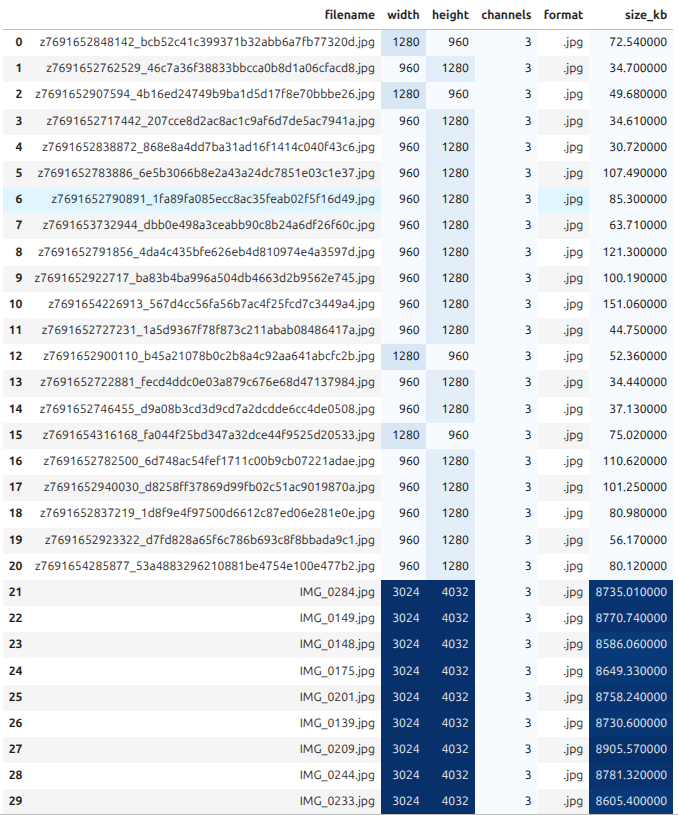
\includegraphics[width=\textwidth]{table_analysis.png}
\caption{ Bảng phân tích thông tin tập ảnh thực nghiệm.}
\end{figure}


\subsection{Chiến lược lấy mẫu và trực quan hóa}

Do tập dữ liệu lớn và các thuật toán như Region Growing tốn nhiều chi phí tính toán, việc trực quan hóa toàn bộ dữ liệu có thể dẫn đến tràn bộ nhớ (Out of memory). Nhóm sử dụng phương pháp lấy mẫu ngẫu nhiên để chọn các tập con phục vụ việc hiển thị.


Ngoài ra, nhóm tiến hành trực quan một số ảnh mẫu để đánh giá các vấn đề thường gặp như:
\begin{itemize}
    \item Ảnh bị nghiêng hoặc méo phối cảnh
    \item Ánh sáng không đồng đều
    \item Bóng đổ hoặc vùng tối
    \item Nhiễu hoặc vùng bị mờ
\end{itemize}

\begin{figure}[H]
\centering
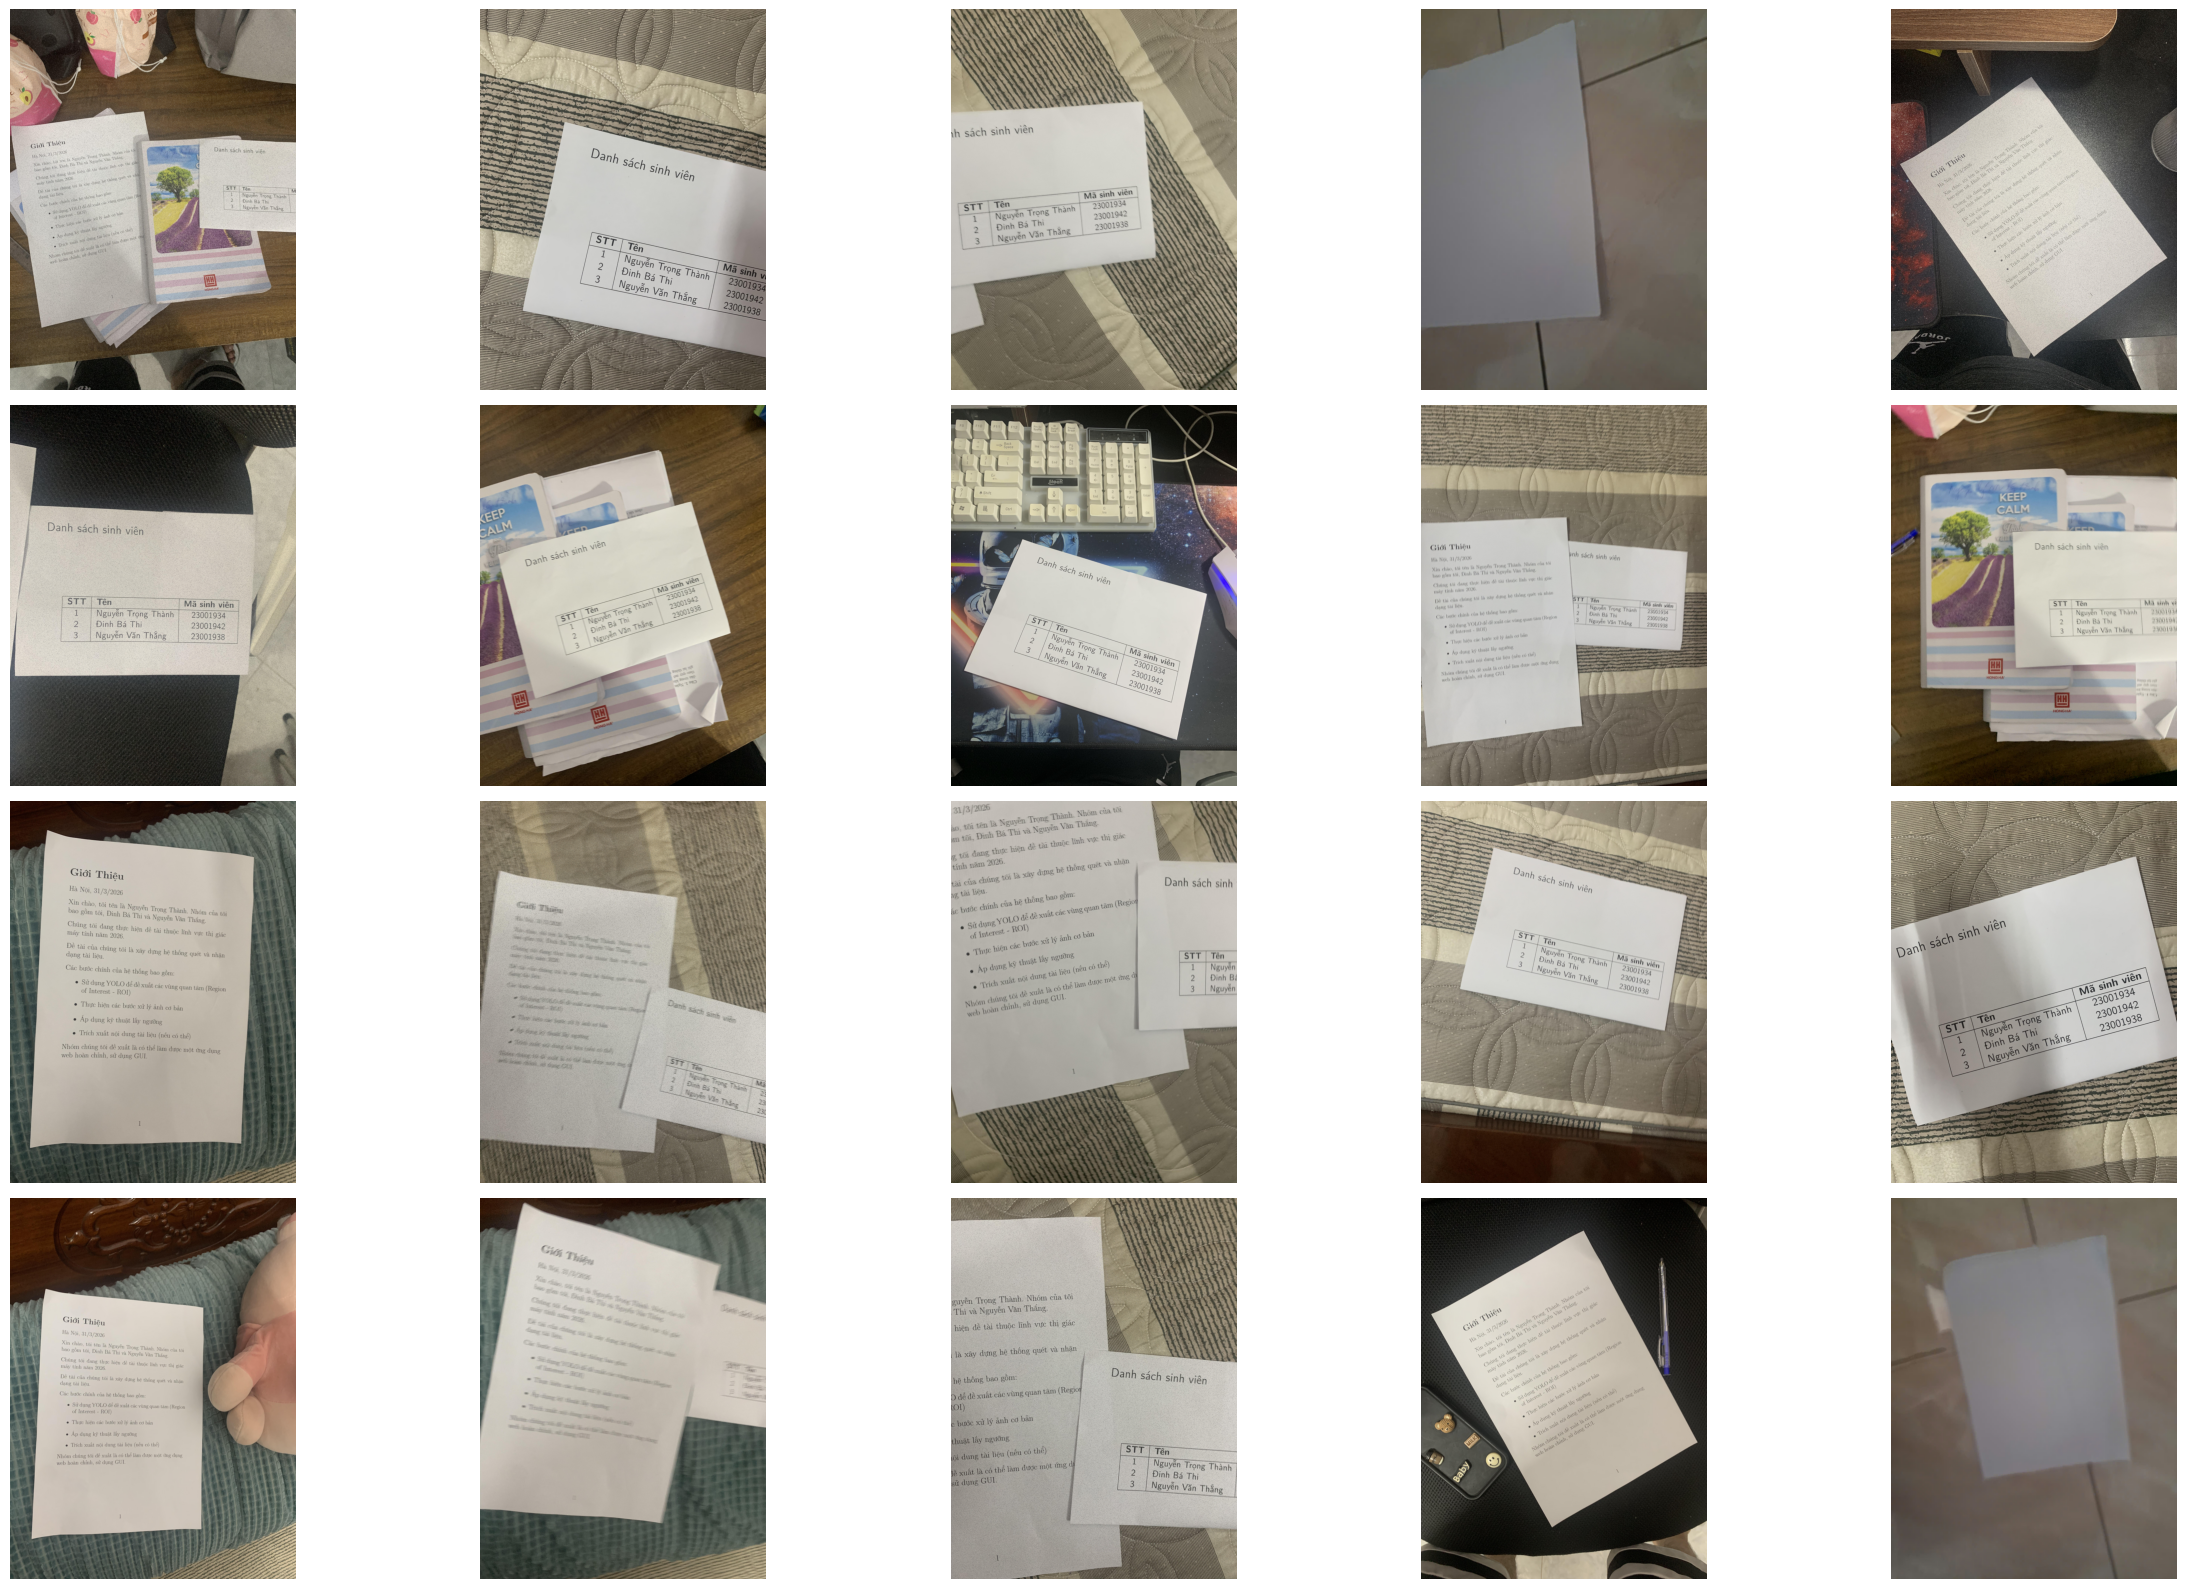
\includegraphics[width=\textwidth]{analysis_img.png}
\caption{Một số ảnh mẫu trong tập dữ liệu}
\end{figure}


\chapter{Thực nghiệm và đánh giá}

\section{Thiết lập thực nghiệm}

Hệ thống được triển khai bằng ngôn ngữ Python với các thư viện chính như OpenCV \cite{opencv_docs}, NumPy và Matplotlib. Các thuật toán phân đoạn và lọc được thiết kế để xử lý dữ liệu với mật độ điểm ảnh lớn. Trong một số trường hợp với các ảnh có độ phân giải $3024 \times 4032$, do giới hạn bộ nhớ heap của Python, nhóm đã chủ động giới hạn số lượng ảnh cho thuật toán duyệt tuần tự (như Region Growing) để phòng tránh hiện tượng Out Of Memory (OOM).

\section{Biểu diễn ảnh qua các hệ màu}

Biểu diễn ảnh qua các hệ màu giúp tách riêng thông tin độ sáng và màu sắc, từ đó xử lý ảnh ổn định hơn trong điều kiện ánh sáng phức tạp. Ảnh được chuyển sang hệ HSV để khai thác kênh V nhằm cân bằng sáng và giảm ảnh hưởng của bóng đổ, đồng thời vẫn giữ được màu sắc gốc của tài liệu.

Ngoài ra, hệ LAB được sử dụng nhờ kênh $L^*$ biểu diễn độ sáng độc lập với màu sắc. Điều này giúp phát hiện mép giấy rõ hơn so với khi chỉ xử lý trực tiếp trên RGB.

Sau khi xử lý, ảnh có thể được chuyển ngược về RGB để các thuật toán như Region Growing tính khoảng cách màu chính xác hơn.
% \section{Biểu diễn ảnh qua các hệ màu}

\subsection{Red - Green - Blue (RGB)}

Dưới đây là biểu diễn trực quan hình ảnh RGB bản gốc.

\begin{figure}[H]
\centering
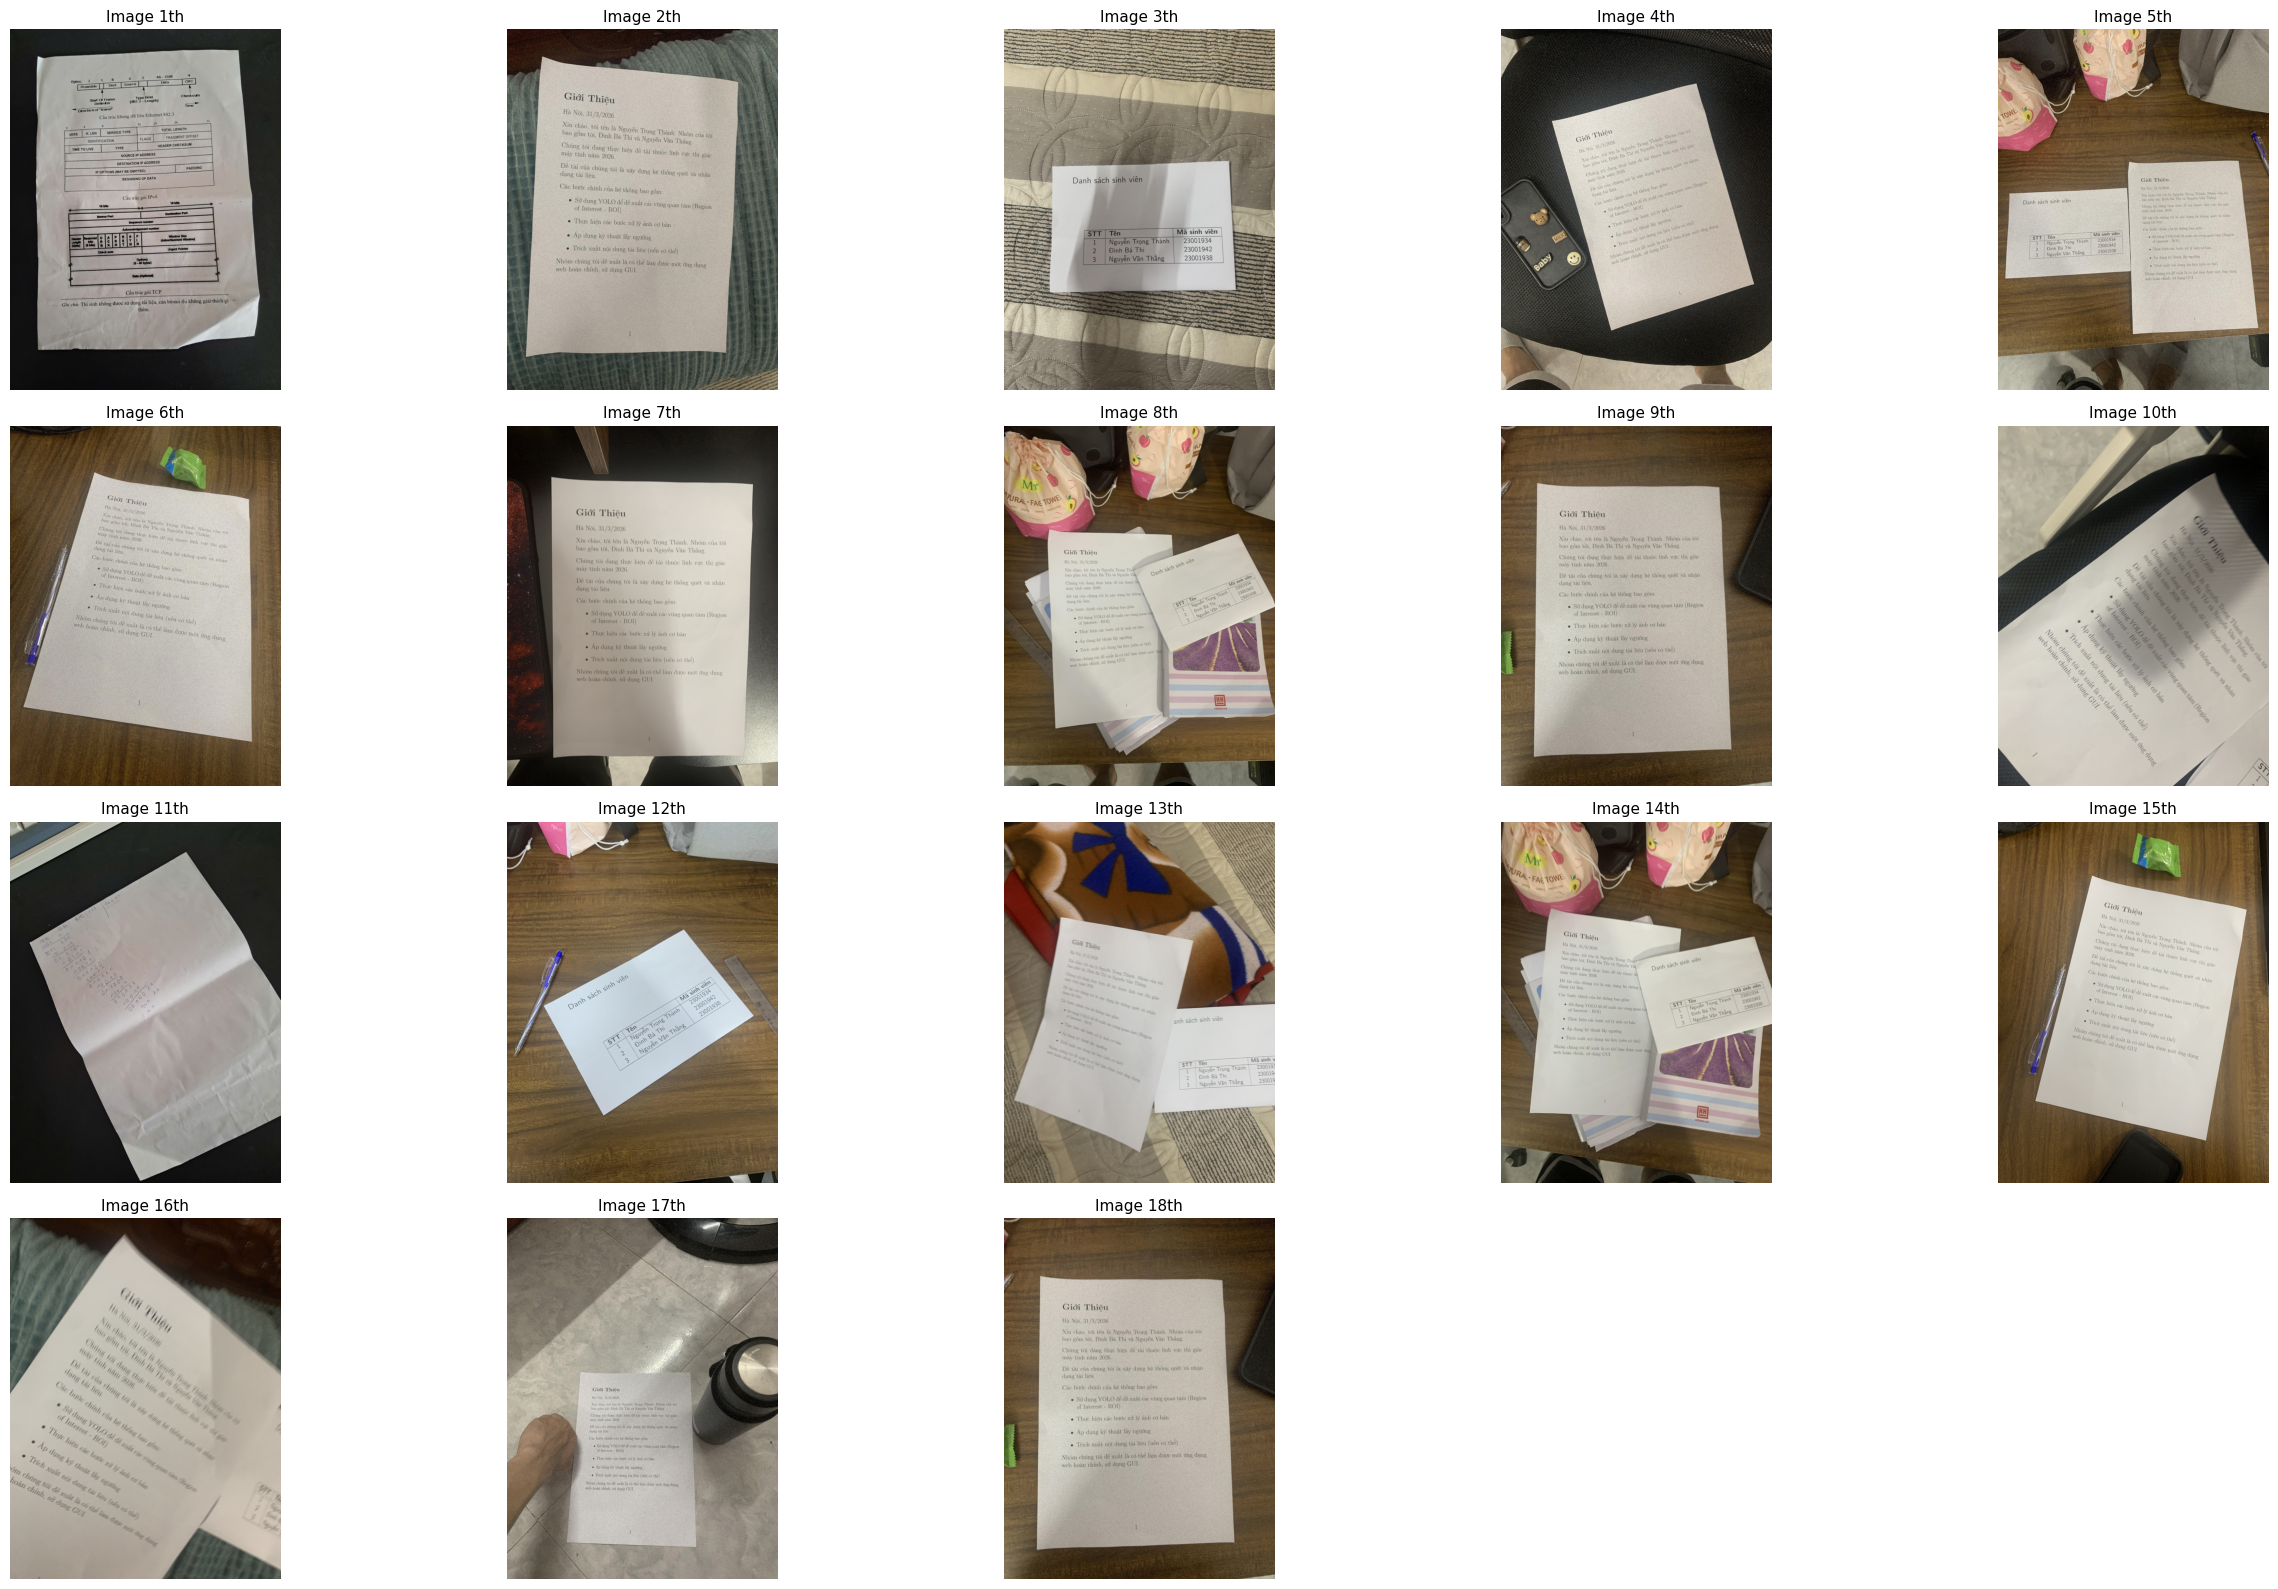
\includegraphics[width=0.9\textwidth]{rgb_visual.png}
\caption{ Một số ảnh trong hệ màu RGB}
\end{figure}

Histogram của từng ảnh trong hệ màu RGB

\begin{figure}[H]
\centering
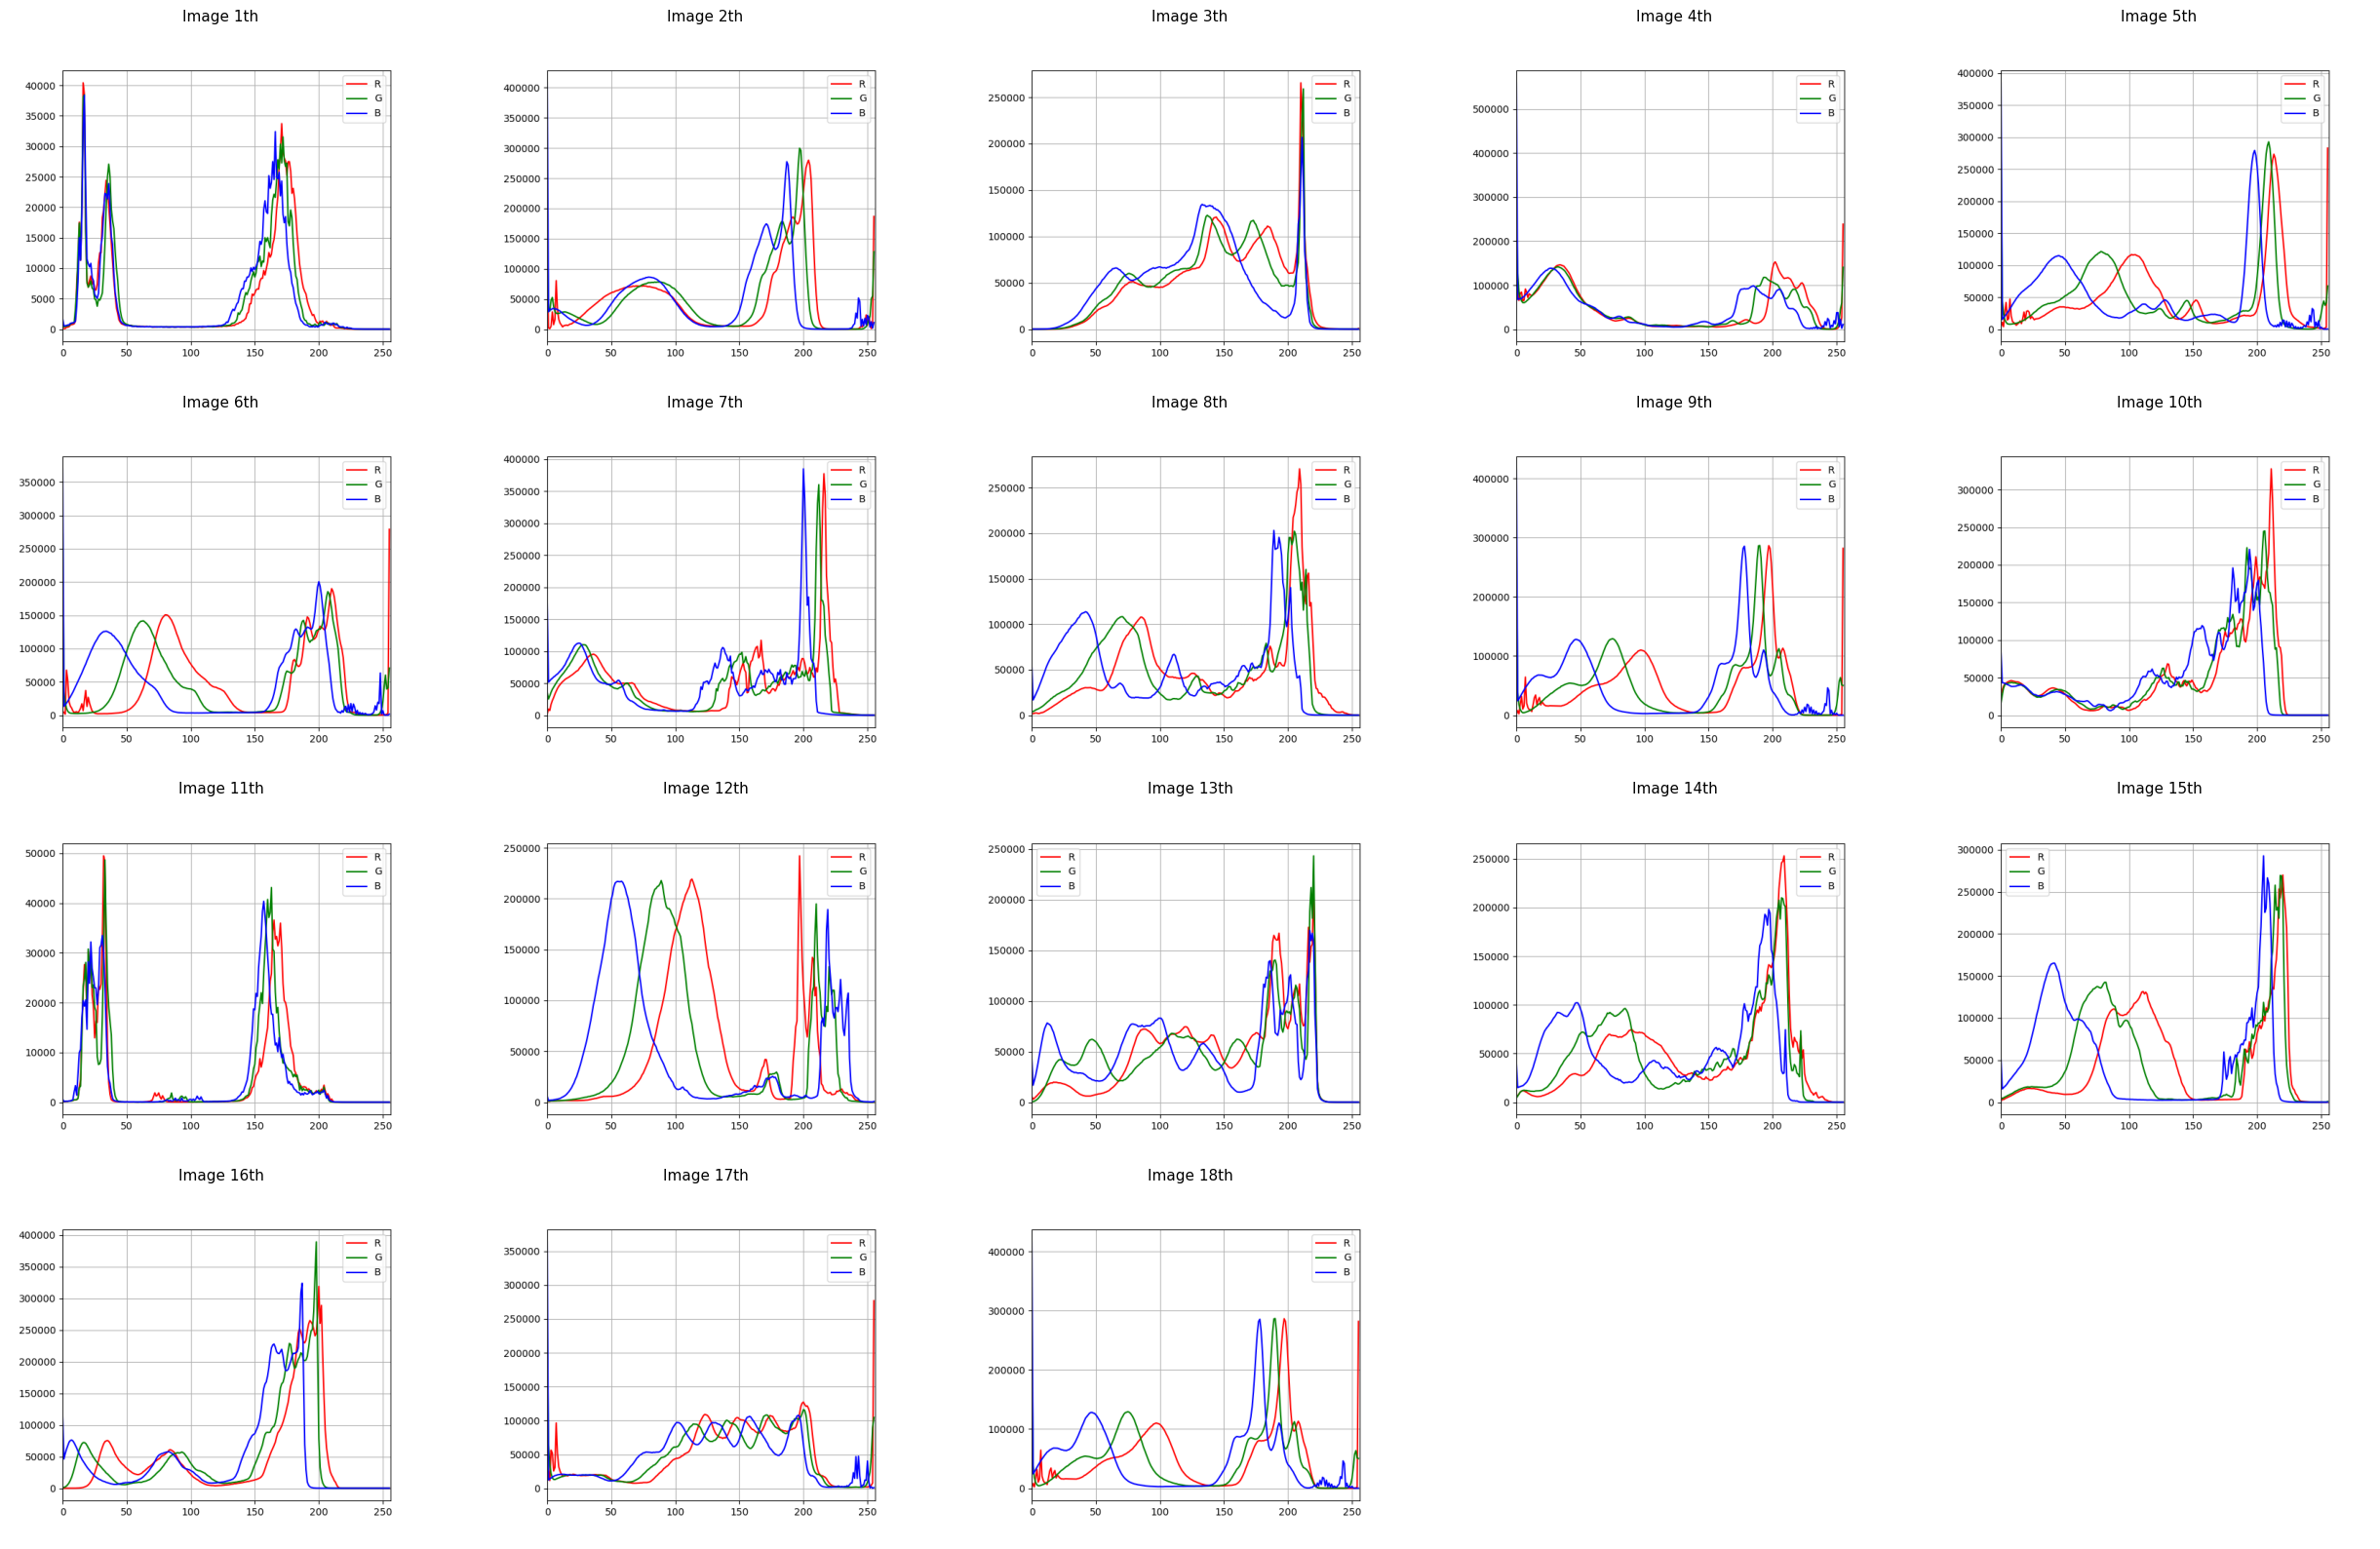
\includegraphics[width=0.9\textwidth]{hist_rgb.png}
\caption{ Histogram của một số ảnh trong hệ màu RGB}
\end{figure}

Phần lớn histogram tập trung ở vùng giá trị cao, khoảng 180-255 trên cả ba kênh R, G, B. Điều này cho thấy nền giấy trắng chiếm diện tích lớn trong ảnh. Một số ảnh có đỉnh histogram gần 255, thể hiện các vùng gần trắng hoàn toàn hoặc bị cháy sáng do ánh sáng mạnh.

Ngược lại, histogram trải rộng trong khoảng 50-180 thường xuất hiện khi ảnh có thêm nền bàn, sàn nhà hoặc vật thể xung quanh.

Sự lệch nhau giữa ba kênh R, G, B cho thấy hiện tượng ám màu do điều kiện chiếu sáng. Các giá trị thấp trong khoảng 0-80 thường tương ứng với bóng đổ, nền tối hoặc chi tiết màu đậm.

\subsection{GRAY}

Một số hình ảnh trực quan của ảnh xám.

\begin{figure}[H]
\centering
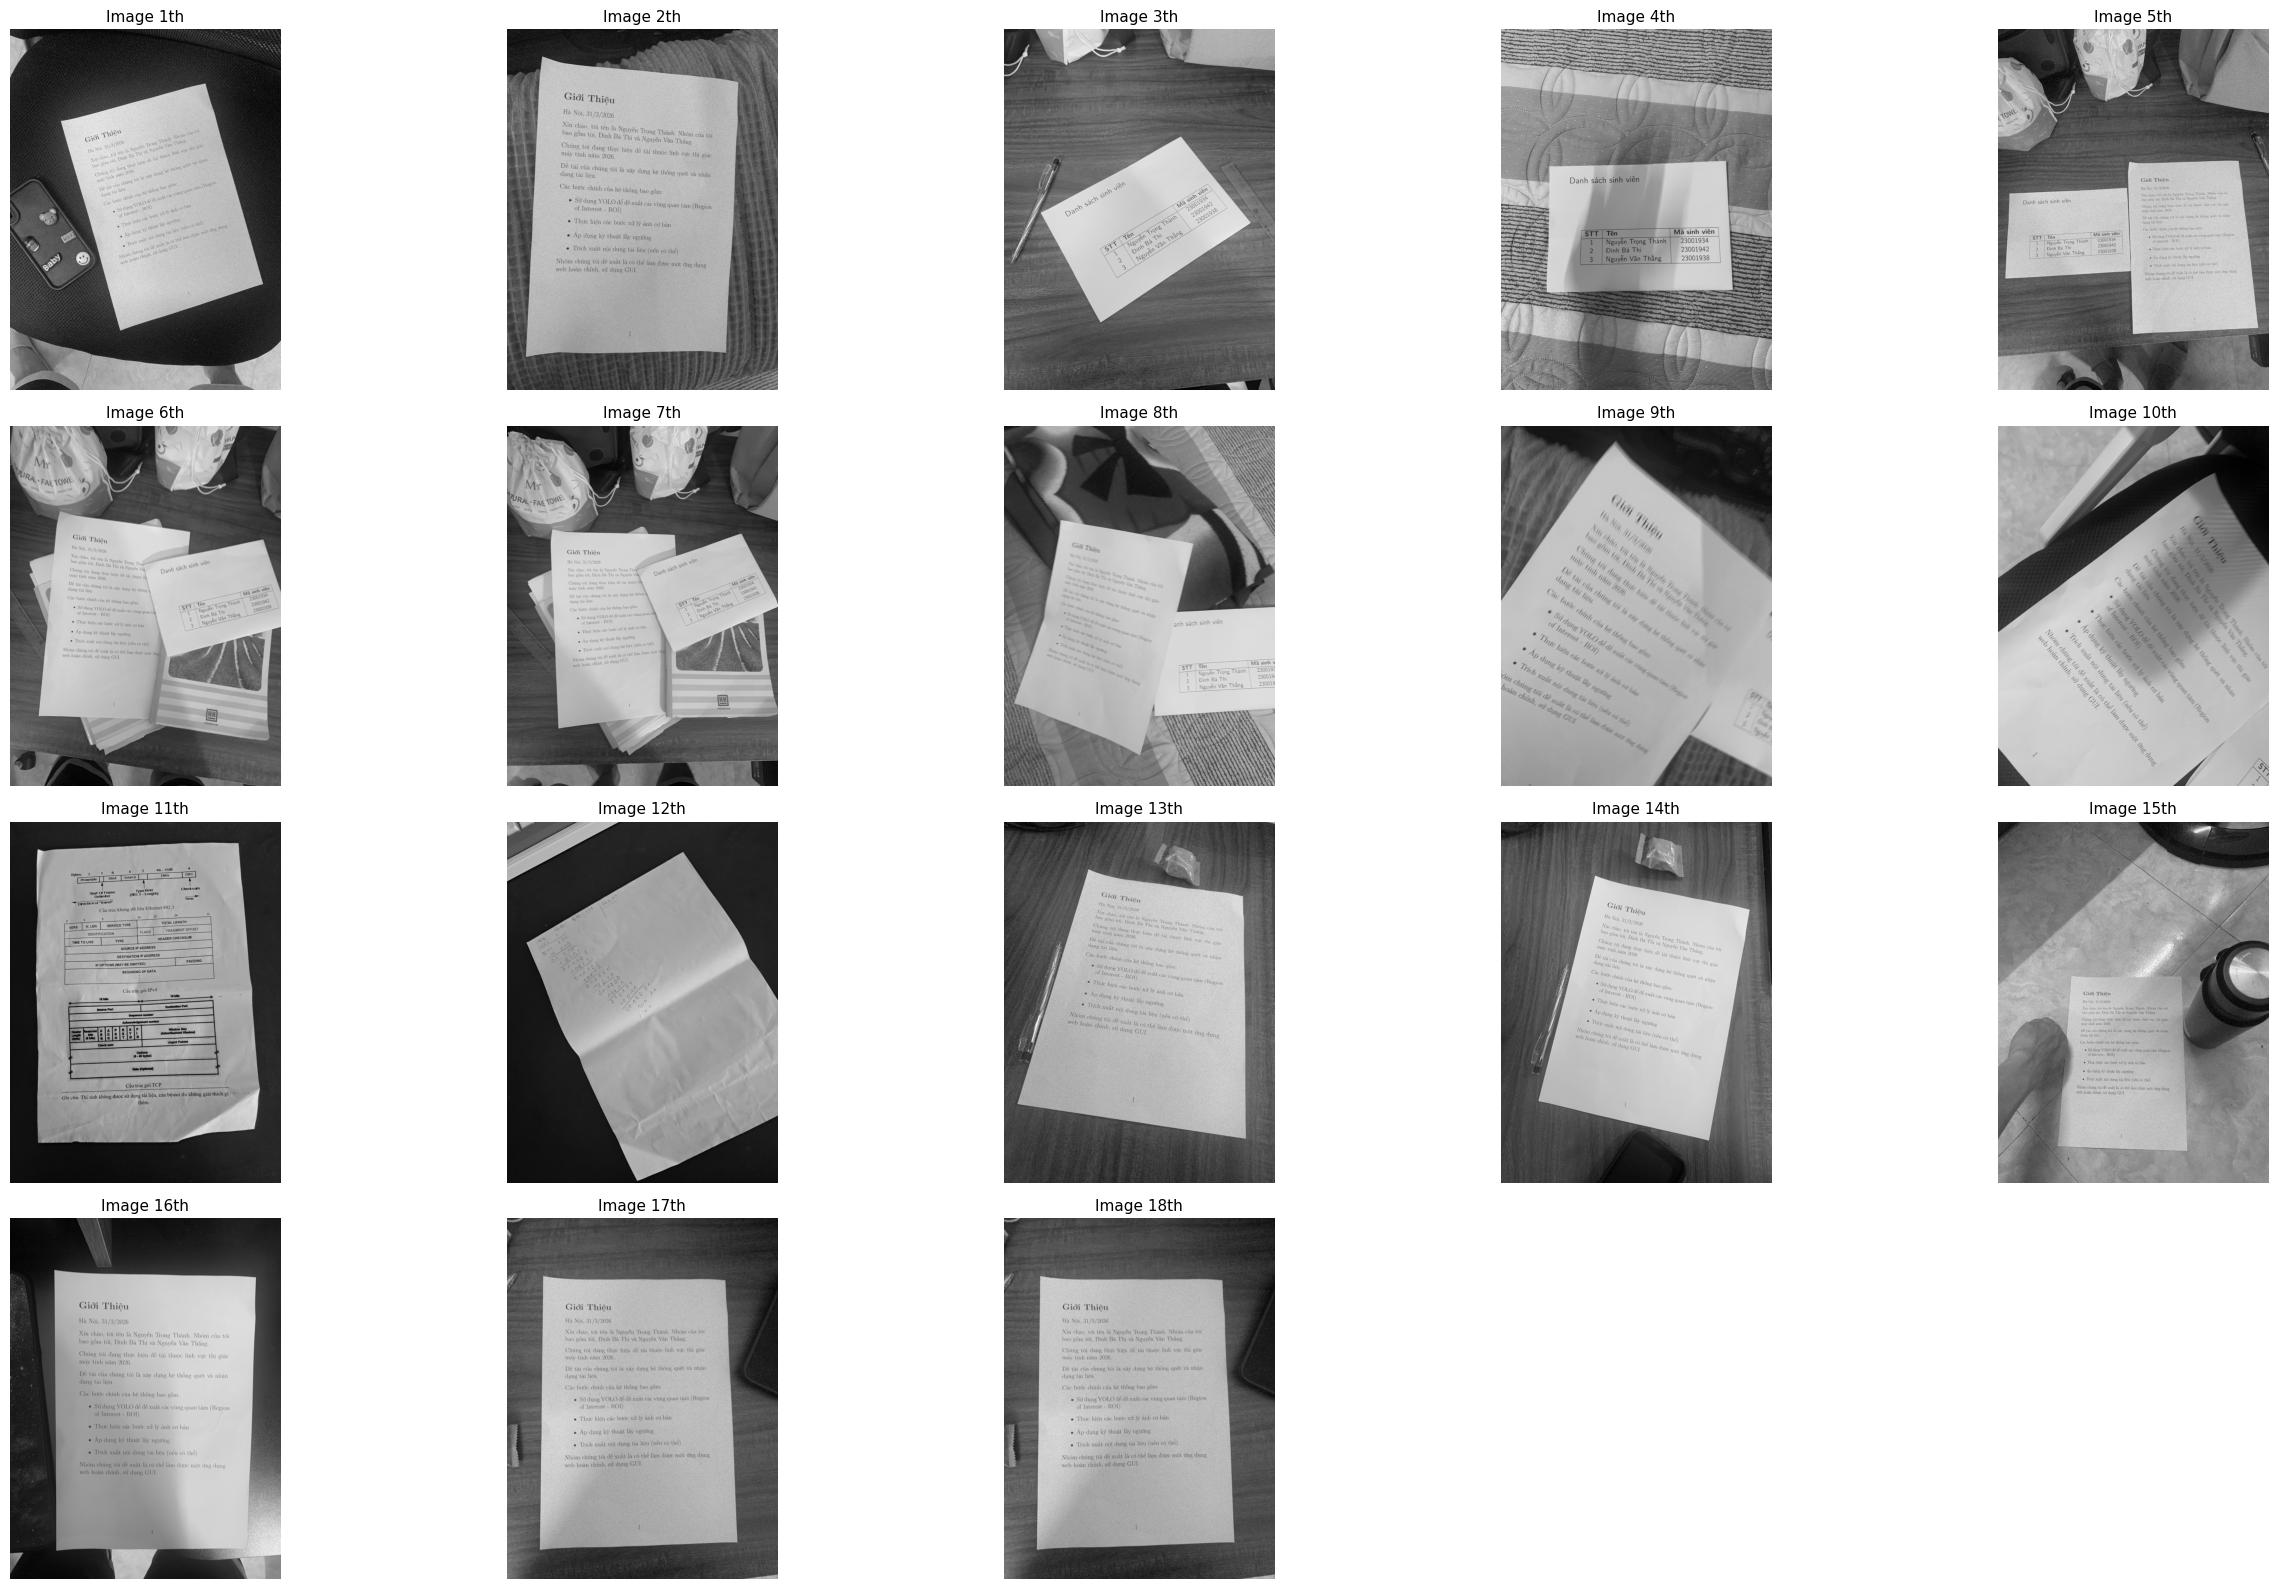
\includegraphics[width=0.9\textwidth]{gray_visual.png}
\caption{Một số ảnh trong hệ màu xám}
\end{figure}

Histogram của một số ảnh xám.

\begin{figure}[H]
\centering
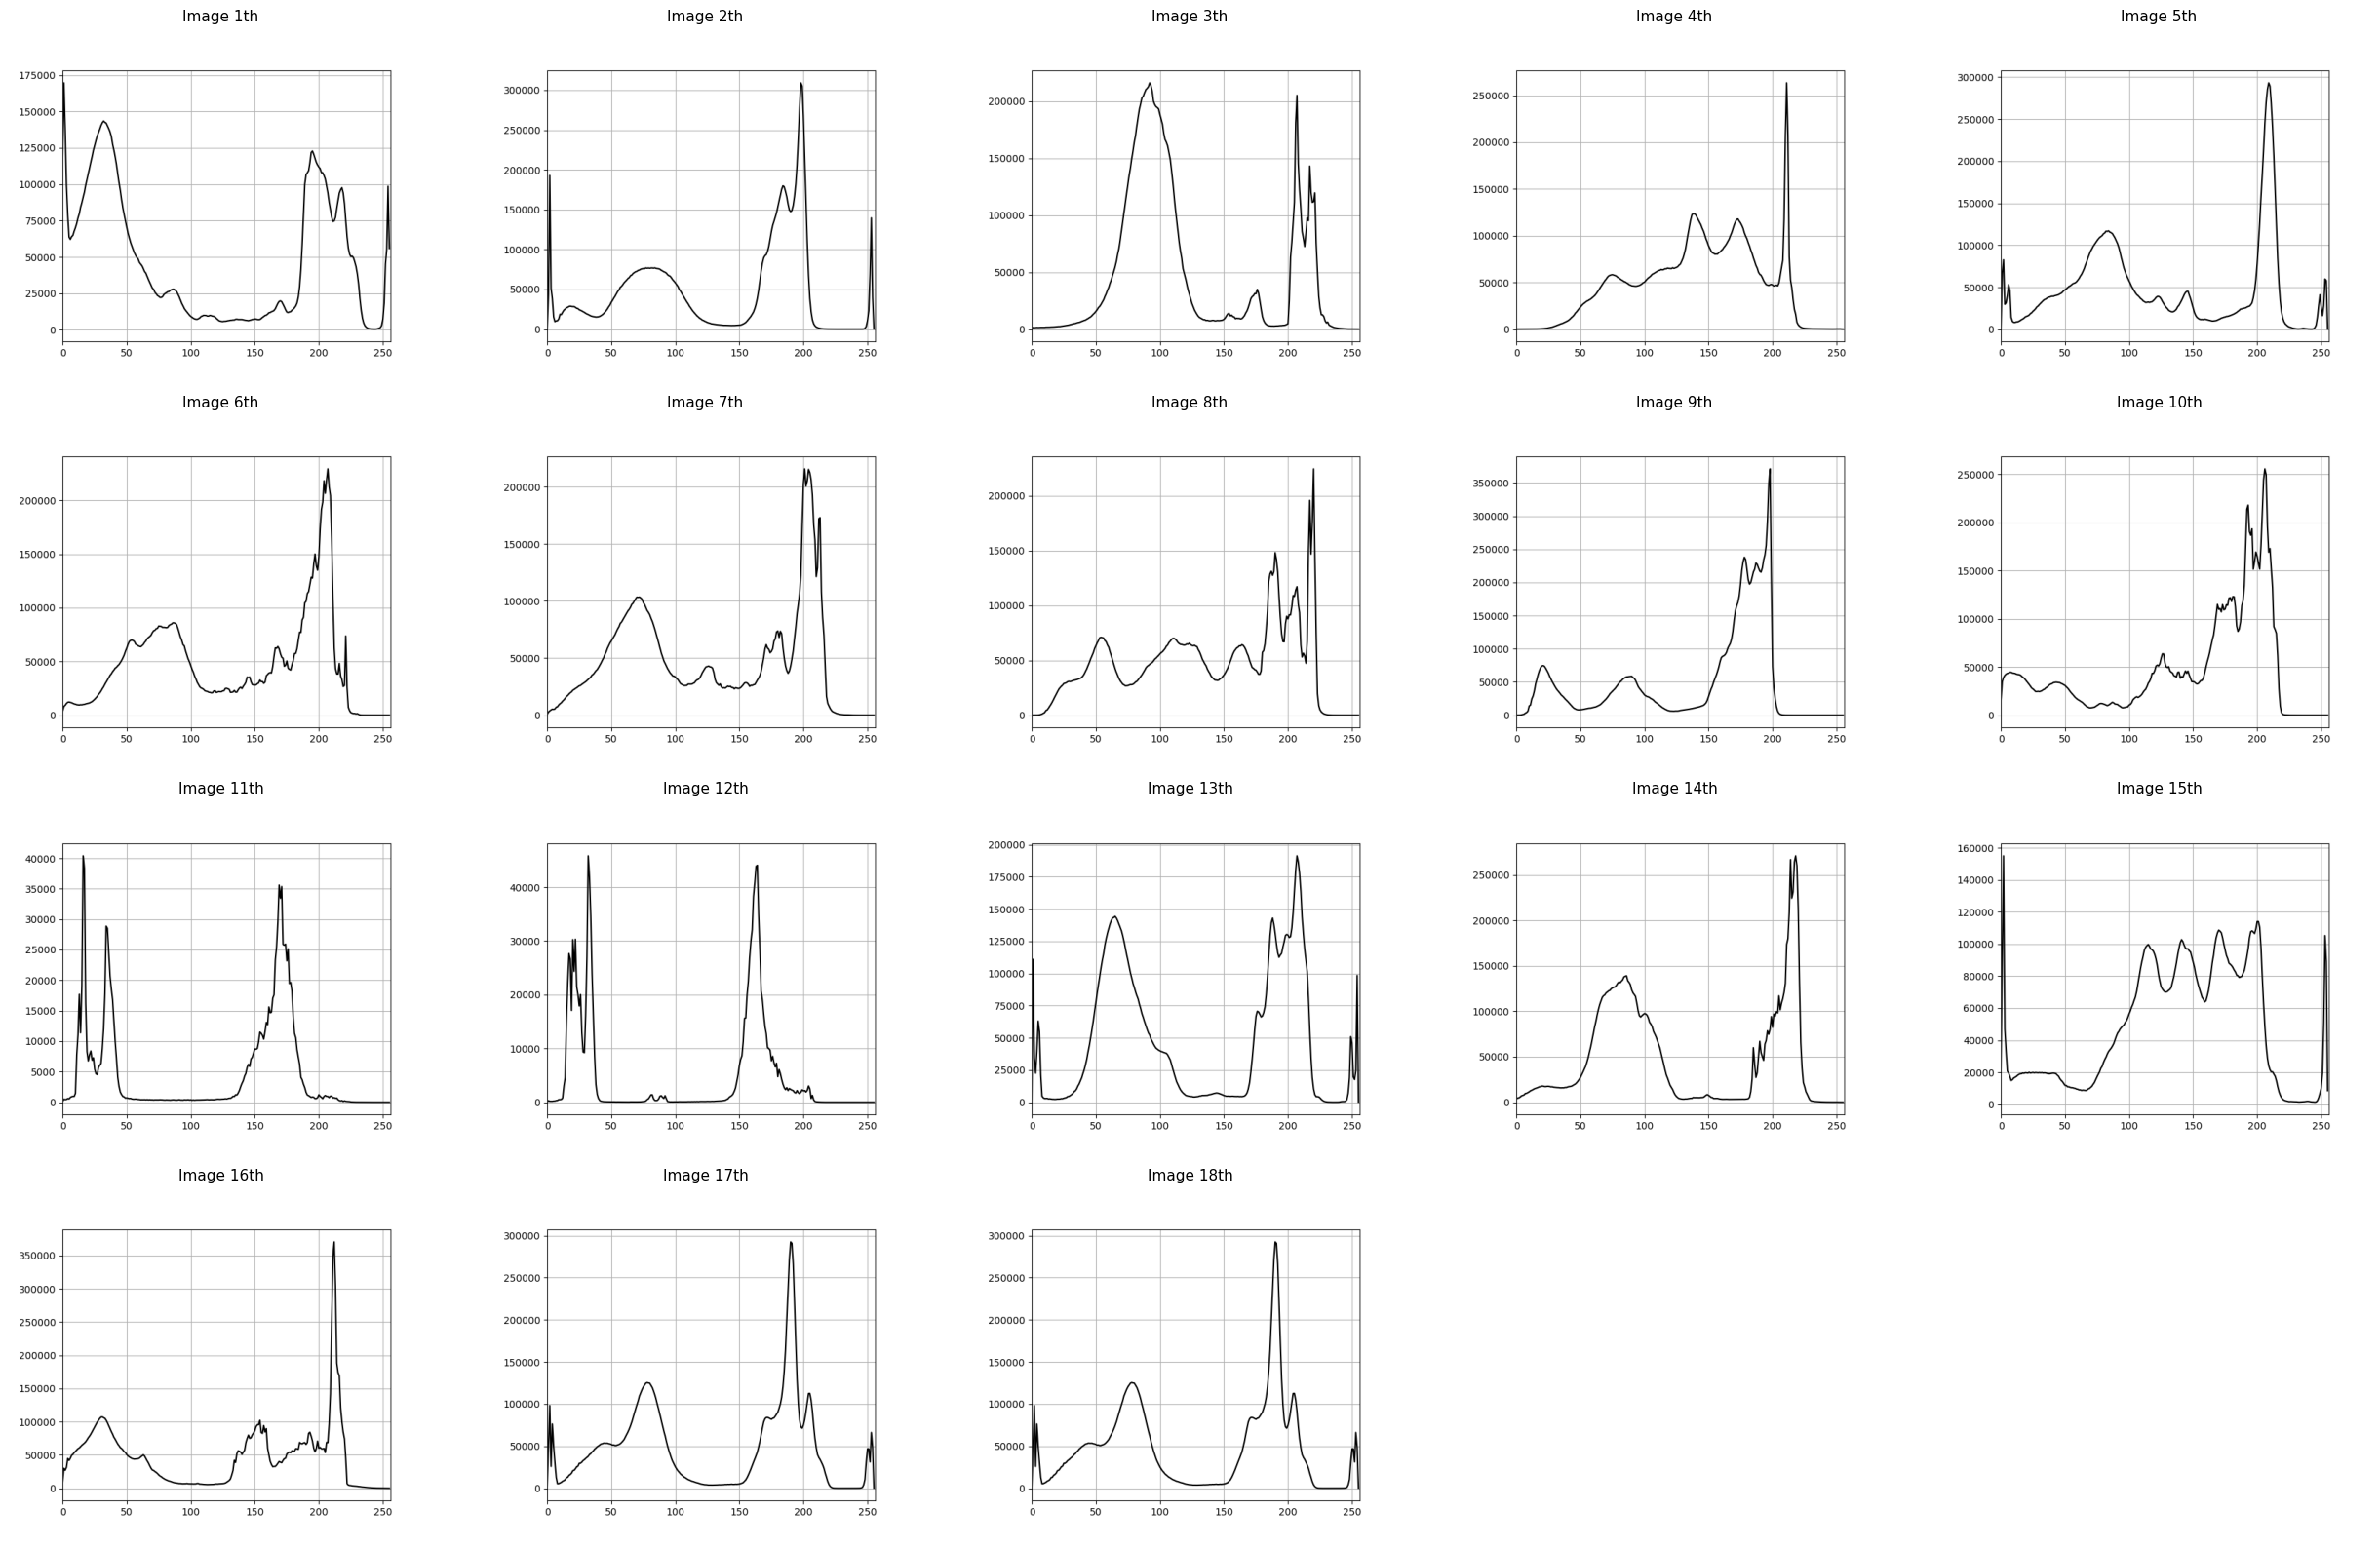
\includegraphics[width=0.9\textwidth]{hist_gray.png}
\caption{Histogram của một số ảnh trong hệ màu xám}
\end{figure}

Histogram của ảnh xám cho thấy phần lớn cường độ tập trung ở vùng sáng, khoảng 180-255. Điều này phù hợp vì giấy trắng chiếm diện tích lớn trong ảnh. Nhiều ảnh còn có đỉnh cao gần 220-255, thể hiện các vùng trắng mạnh hoặc bị cháy sáng do ánh đèn, flash.

Một số ảnh có histogram trải rộng từ vùng tối đến vùng sáng, ví dụ Image 4th, 6th, 9th, 20th, do ảnh chứa nhiều nền bàn, sàn nhà hoặc bóng đổ. Ngược lại, các ảnh có hai vùng histogram tách biệt rõ giữa vùng tối của chữ và vùng sáng của giấy thường dễ áp dụng threshold và scan document hơn.

Các ảnh có histogram phức tạp hoặc nhiều đỉnh liên tiếp như Image 16th, 20th, 25th thường khó xử lý hơn do ánh sáng không đều, nhiều vật thể nền hoặc bóng đổ.

\subsection{HSV}

Một số hình ảnh trực quan của ảnh trong hệ màu HSV.

\begin{figure}[H]
\centering
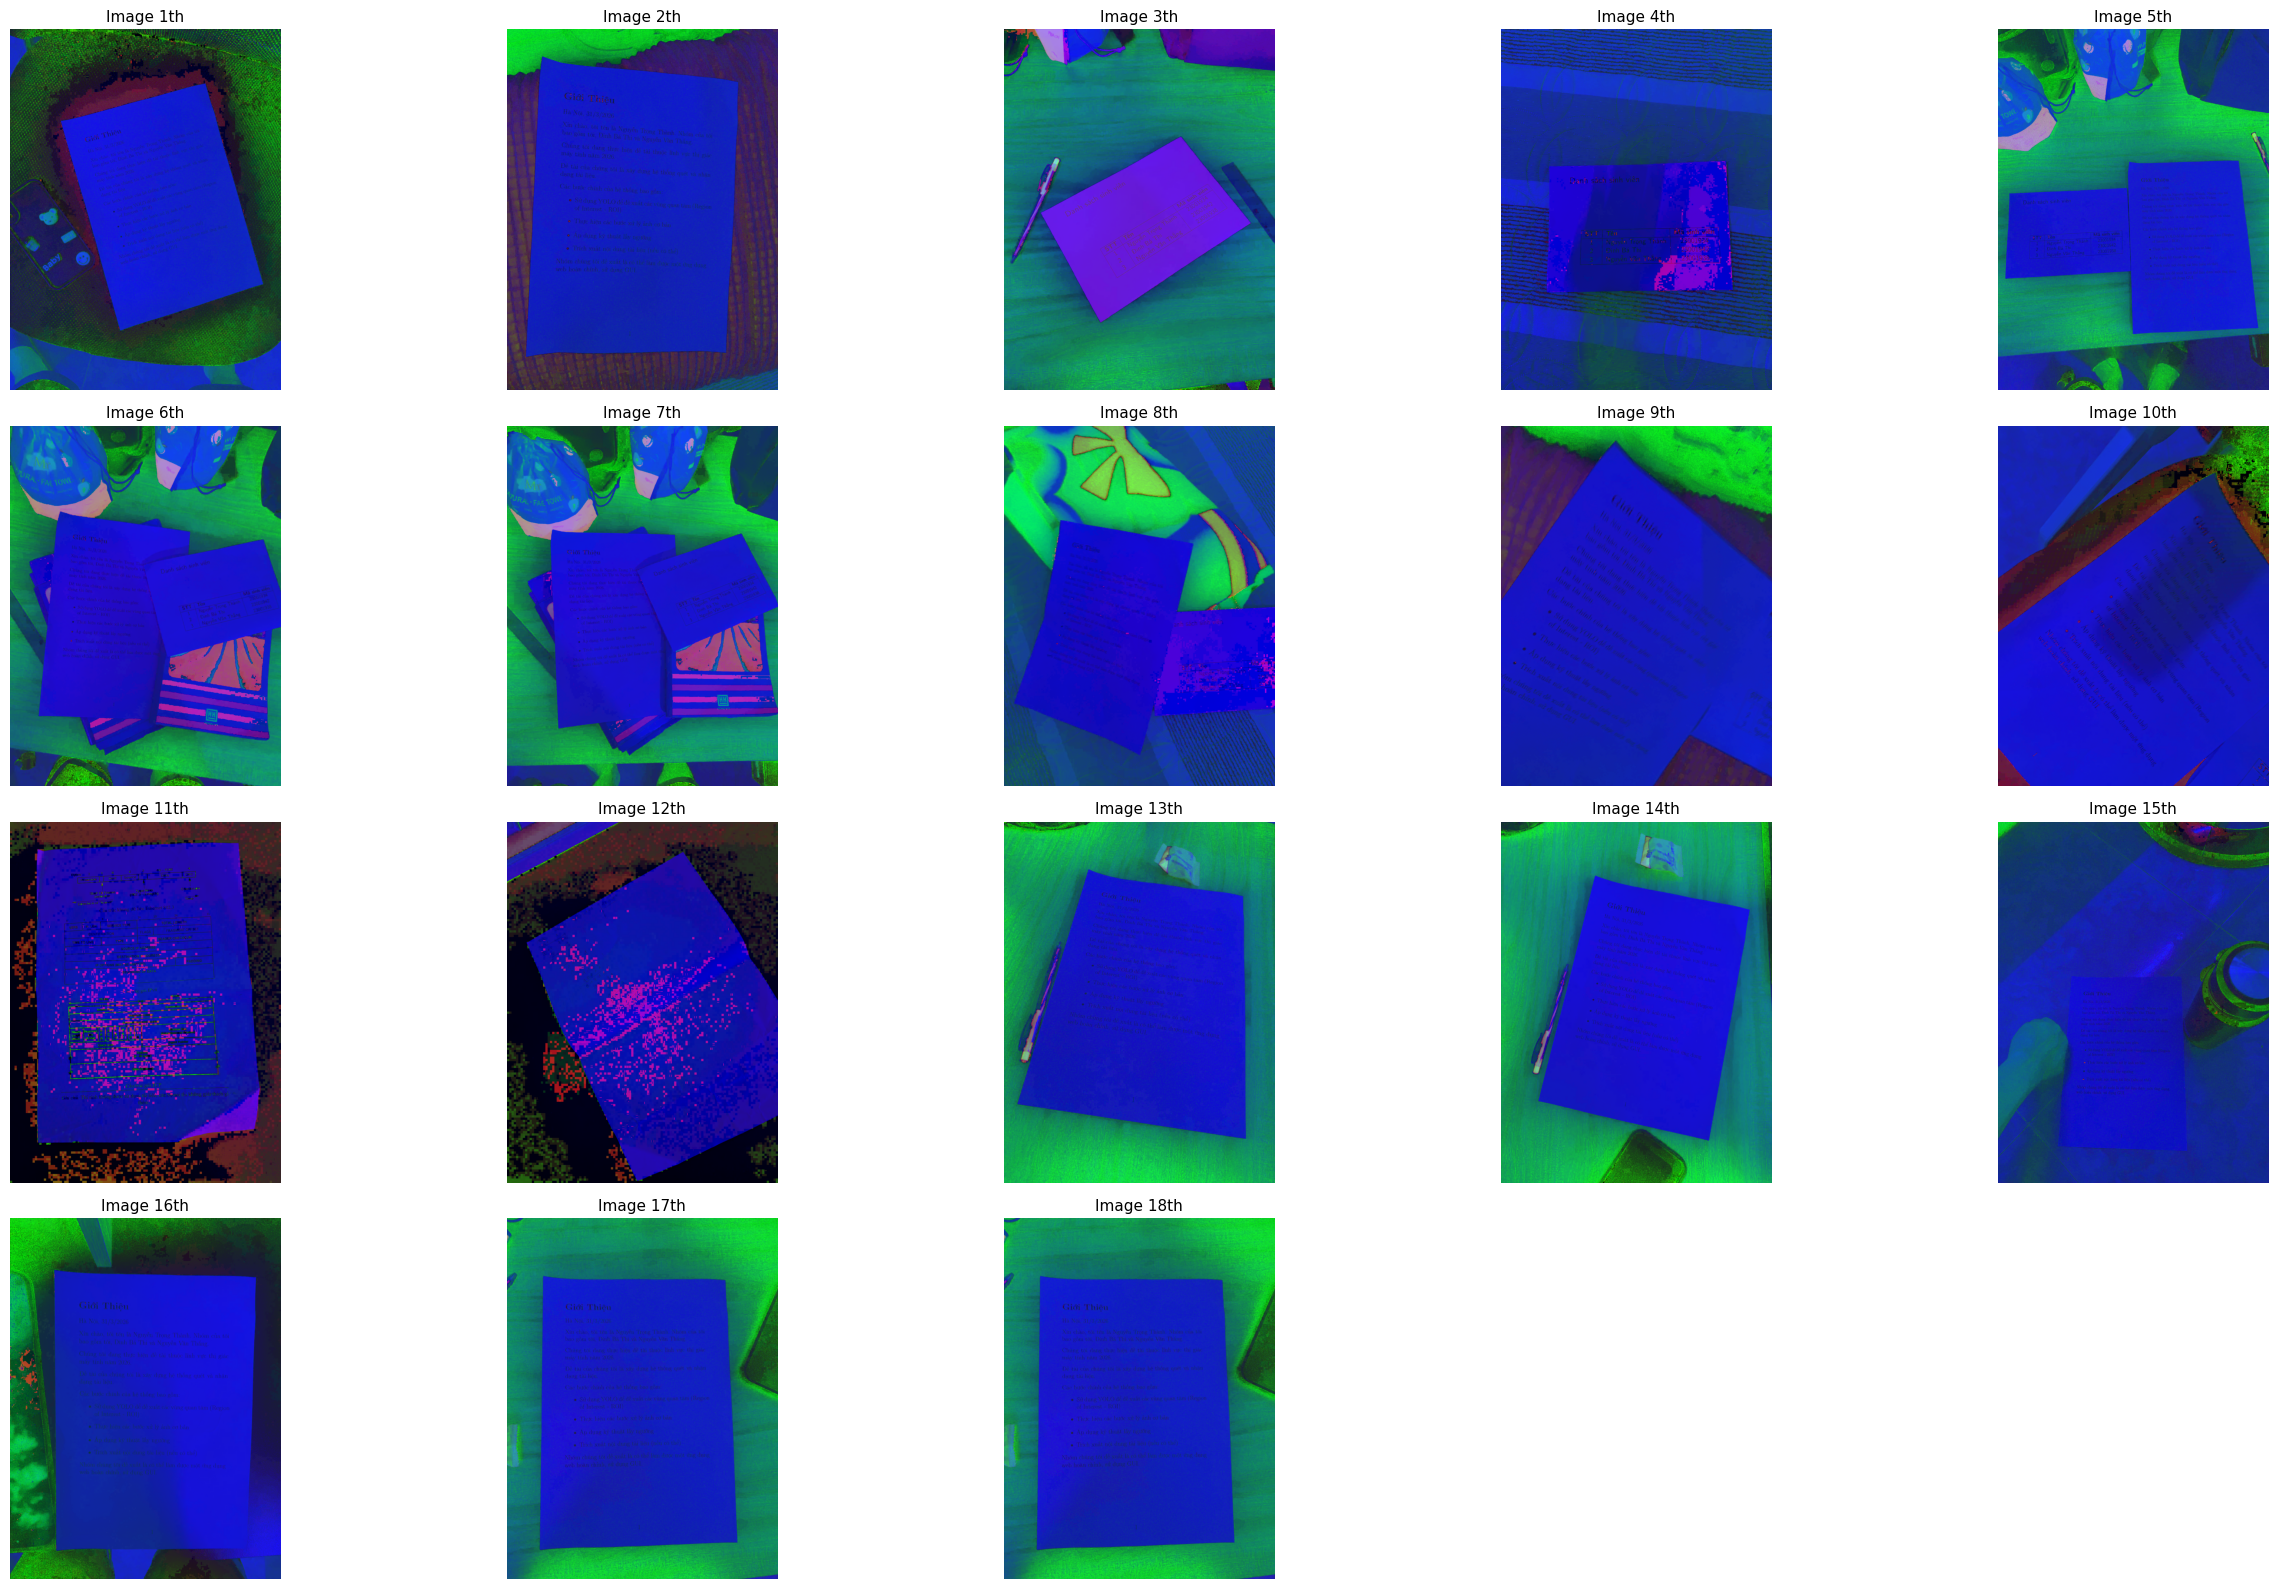
\includegraphics[width=0.9\textwidth]{hsv_visual.png}
\caption{Một số ảnh trong hệ màu HSV}
\end{figure}

Histogram của một số ảnh trong hệ màu HSV.

\begin{figure}[H]
\centering
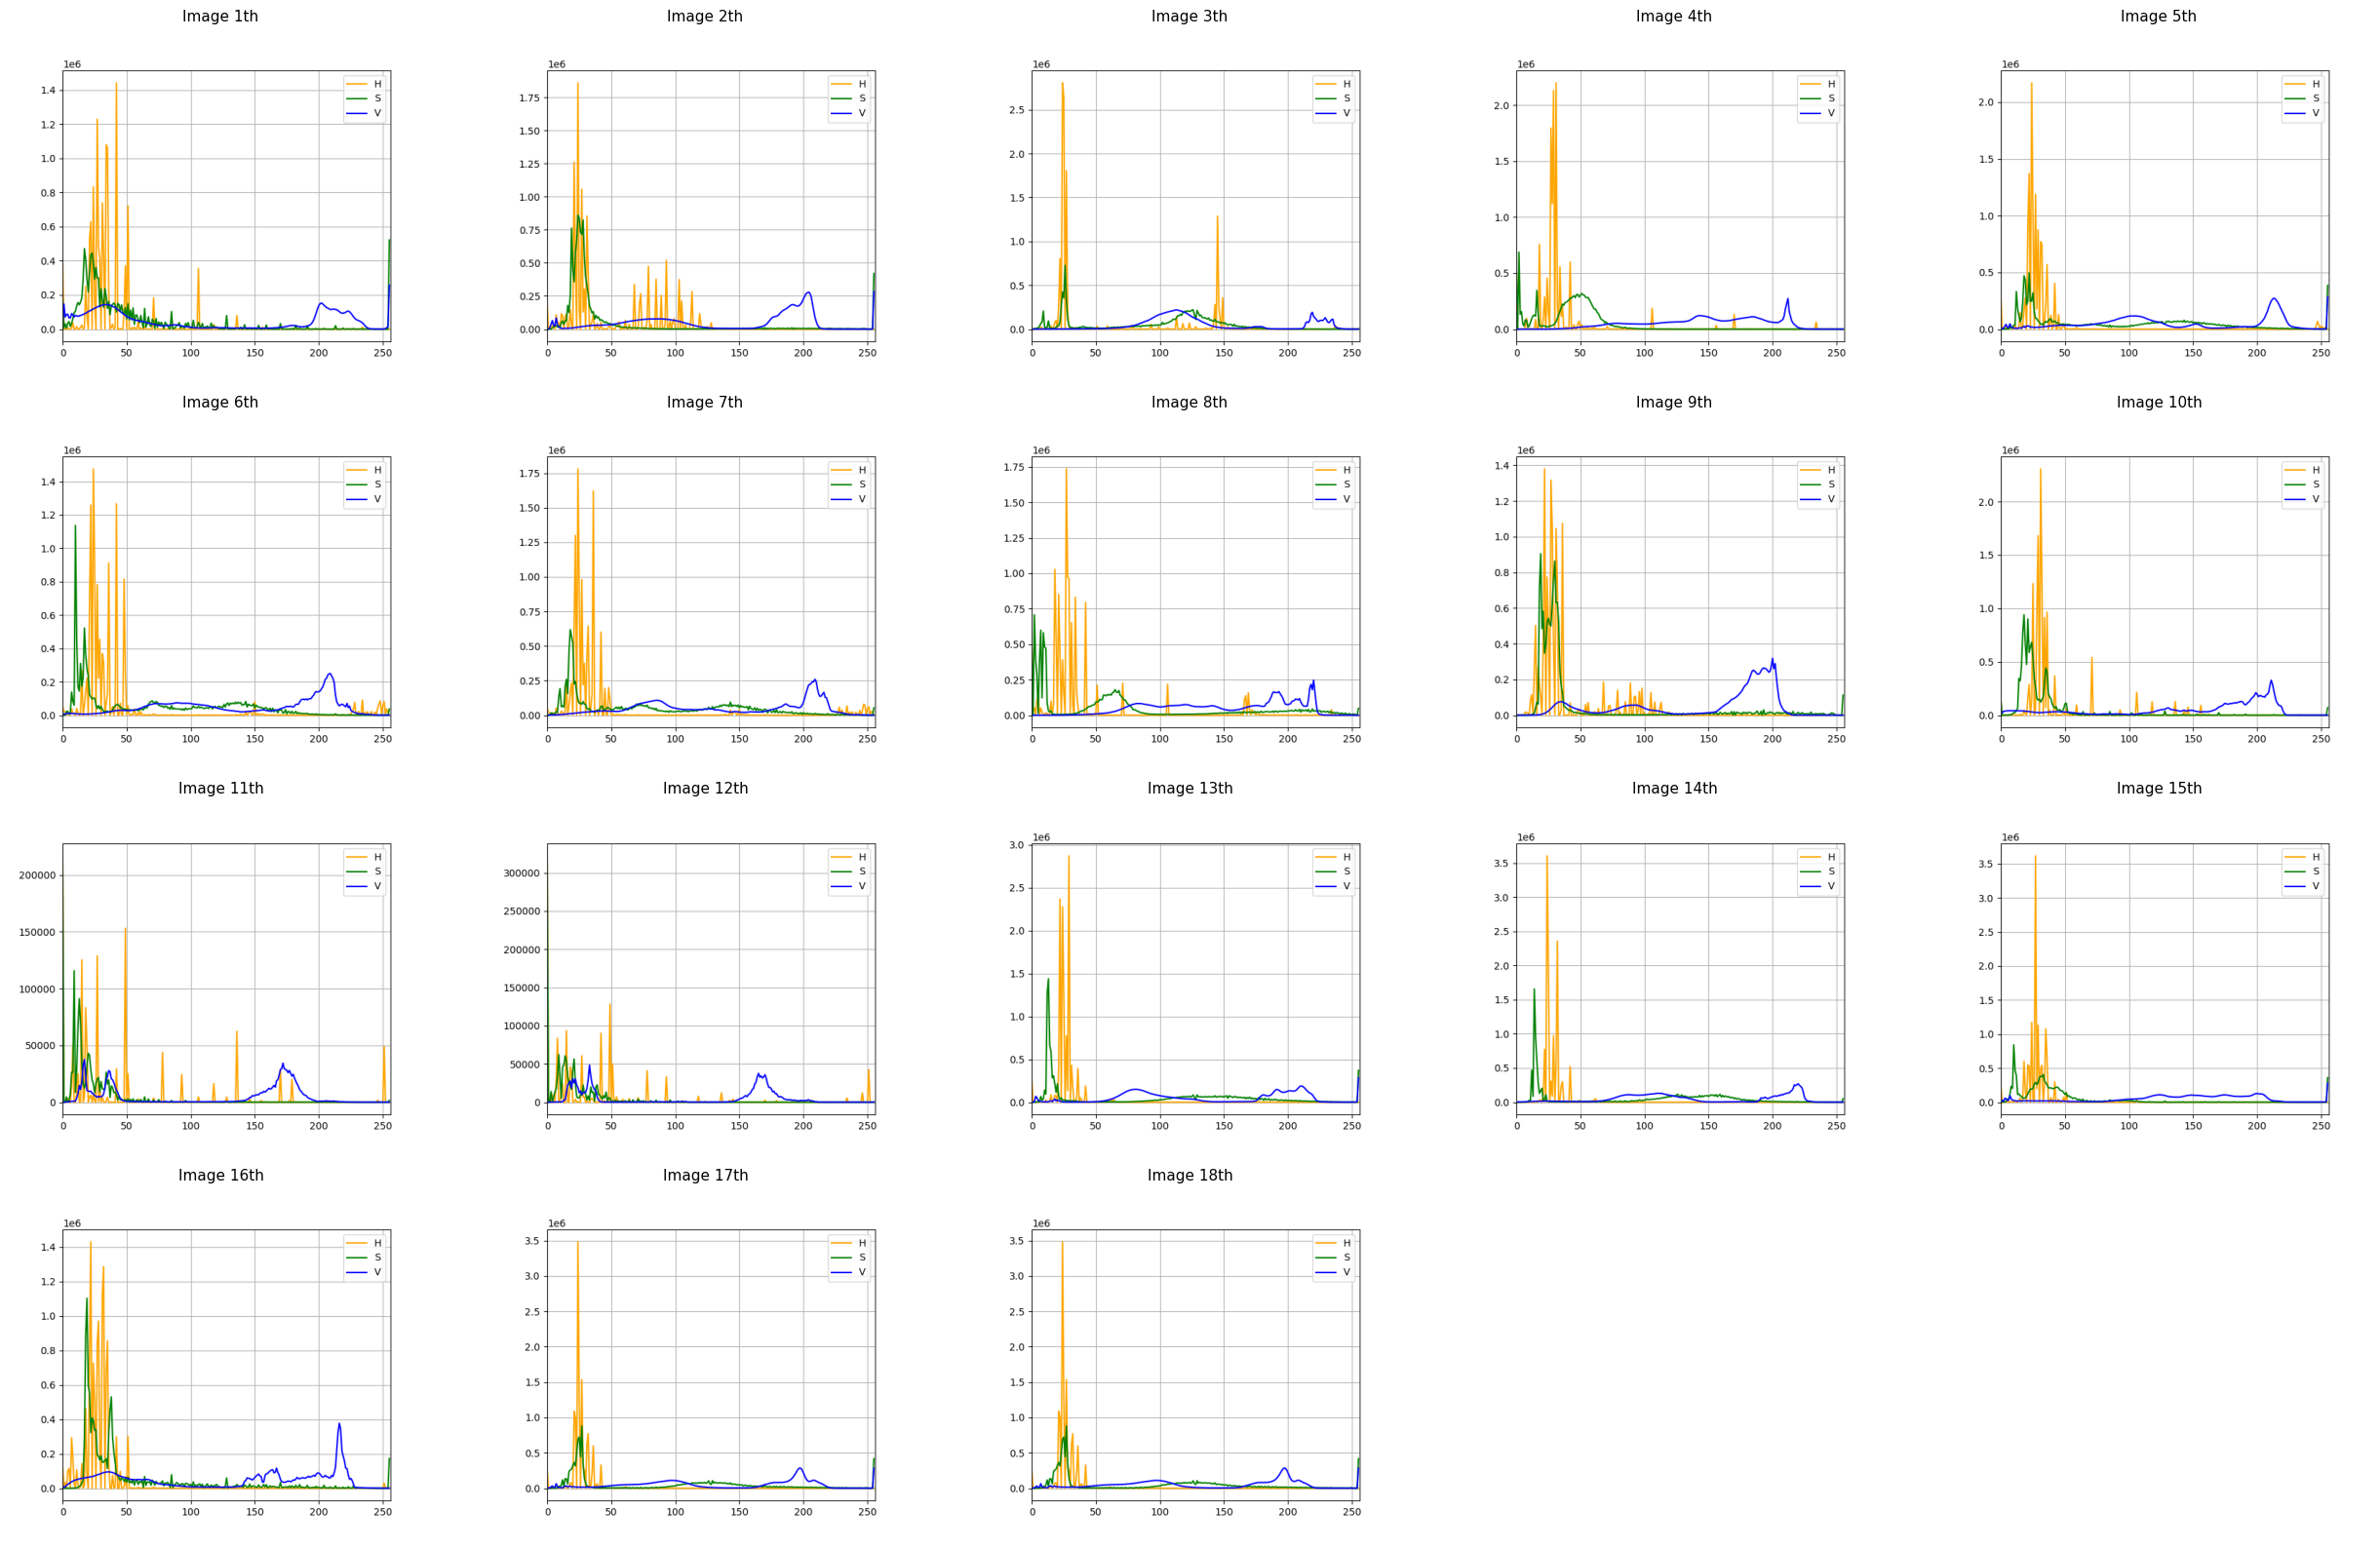
\includegraphics[width=0.9\textwidth]{hist_hsv.png}
\caption{Histogram của một số ảnh trong hệ màu HSV}
\end{figure}

Histogram trong không gian màu HSV thể hiện rõ đặc trưng của tập ảnh tài liệu. Kênh H của phần lớn ảnh tập trung ở vùng giá trị thấp, cho thấy màu sắc trong ảnh không quá đa dạng, chủ yếu là các tông gần trắng, xám, nâu hoặc xanh nhẹ từ nền và giấy.

Kênh S thường có đỉnh rất cao gần 0, chứng tỏ phần lớn vùng ảnh có độ bão hòa thấp, gần với màu trắng hoặc xám. Đây là đặc trưng phù hợp với ảnh scan tài liệu vì giấy trắng và chữ đen hầu như không chứa màu mạnh.

Kênh V của hầu hết ảnh tập trung ở vùng giá trị cao, khoảng 180-255, cho thấy ảnh có độ sáng lớn do nền giấy trắng chiếm diện tích chính. Tuy nhiên, một số ảnh có histogram kênh S hoặc V trải rộng hơn, cho thấy sự xuất hiện của vật thể màu, nền phức tạp, ánh sáng không đồng đều hoặc bóng đổ.

\subsection{LAB}

Một số hình ảnh trực quan của ảnh trong hệ màu LAB.

\begin{figure}[H]
\centering
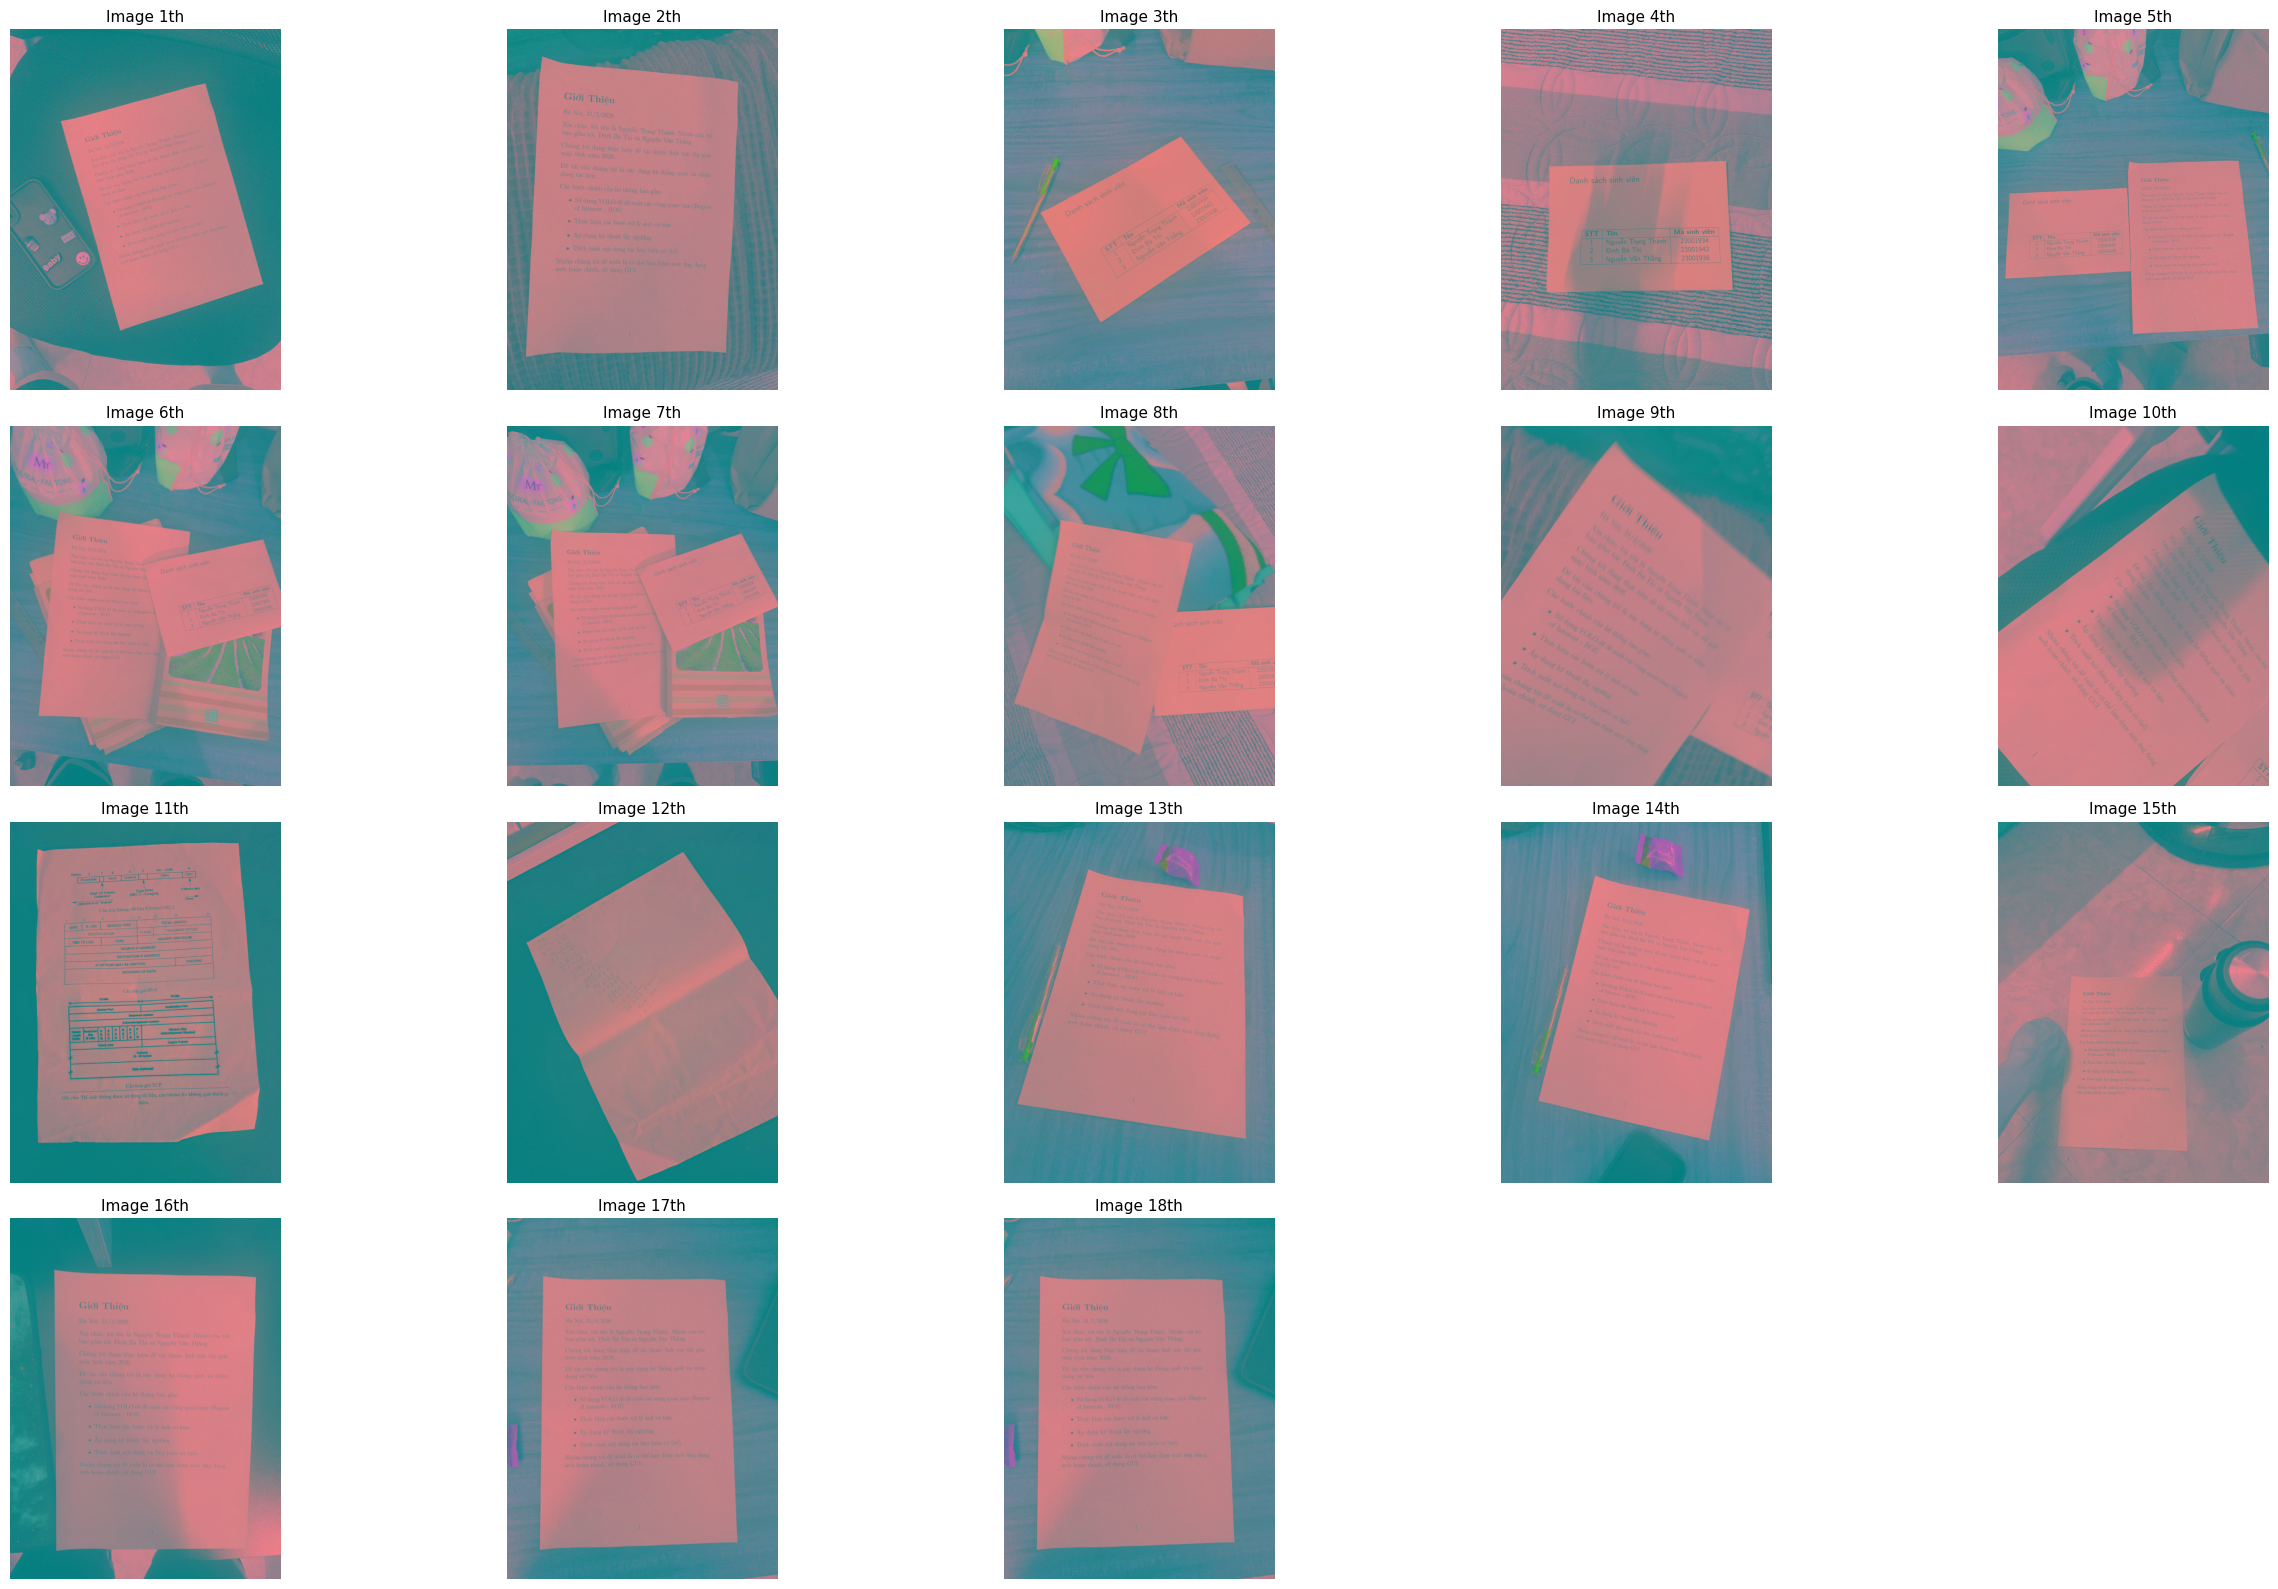
\includegraphics[width=0.9\textwidth]{lab_visual.png}
\caption{Một số ảnh trong hệ màu LAB}
\end{figure}

Histogram của một số ảnh trong hệ màu LAB.

\begin{figure}[H]
\centering
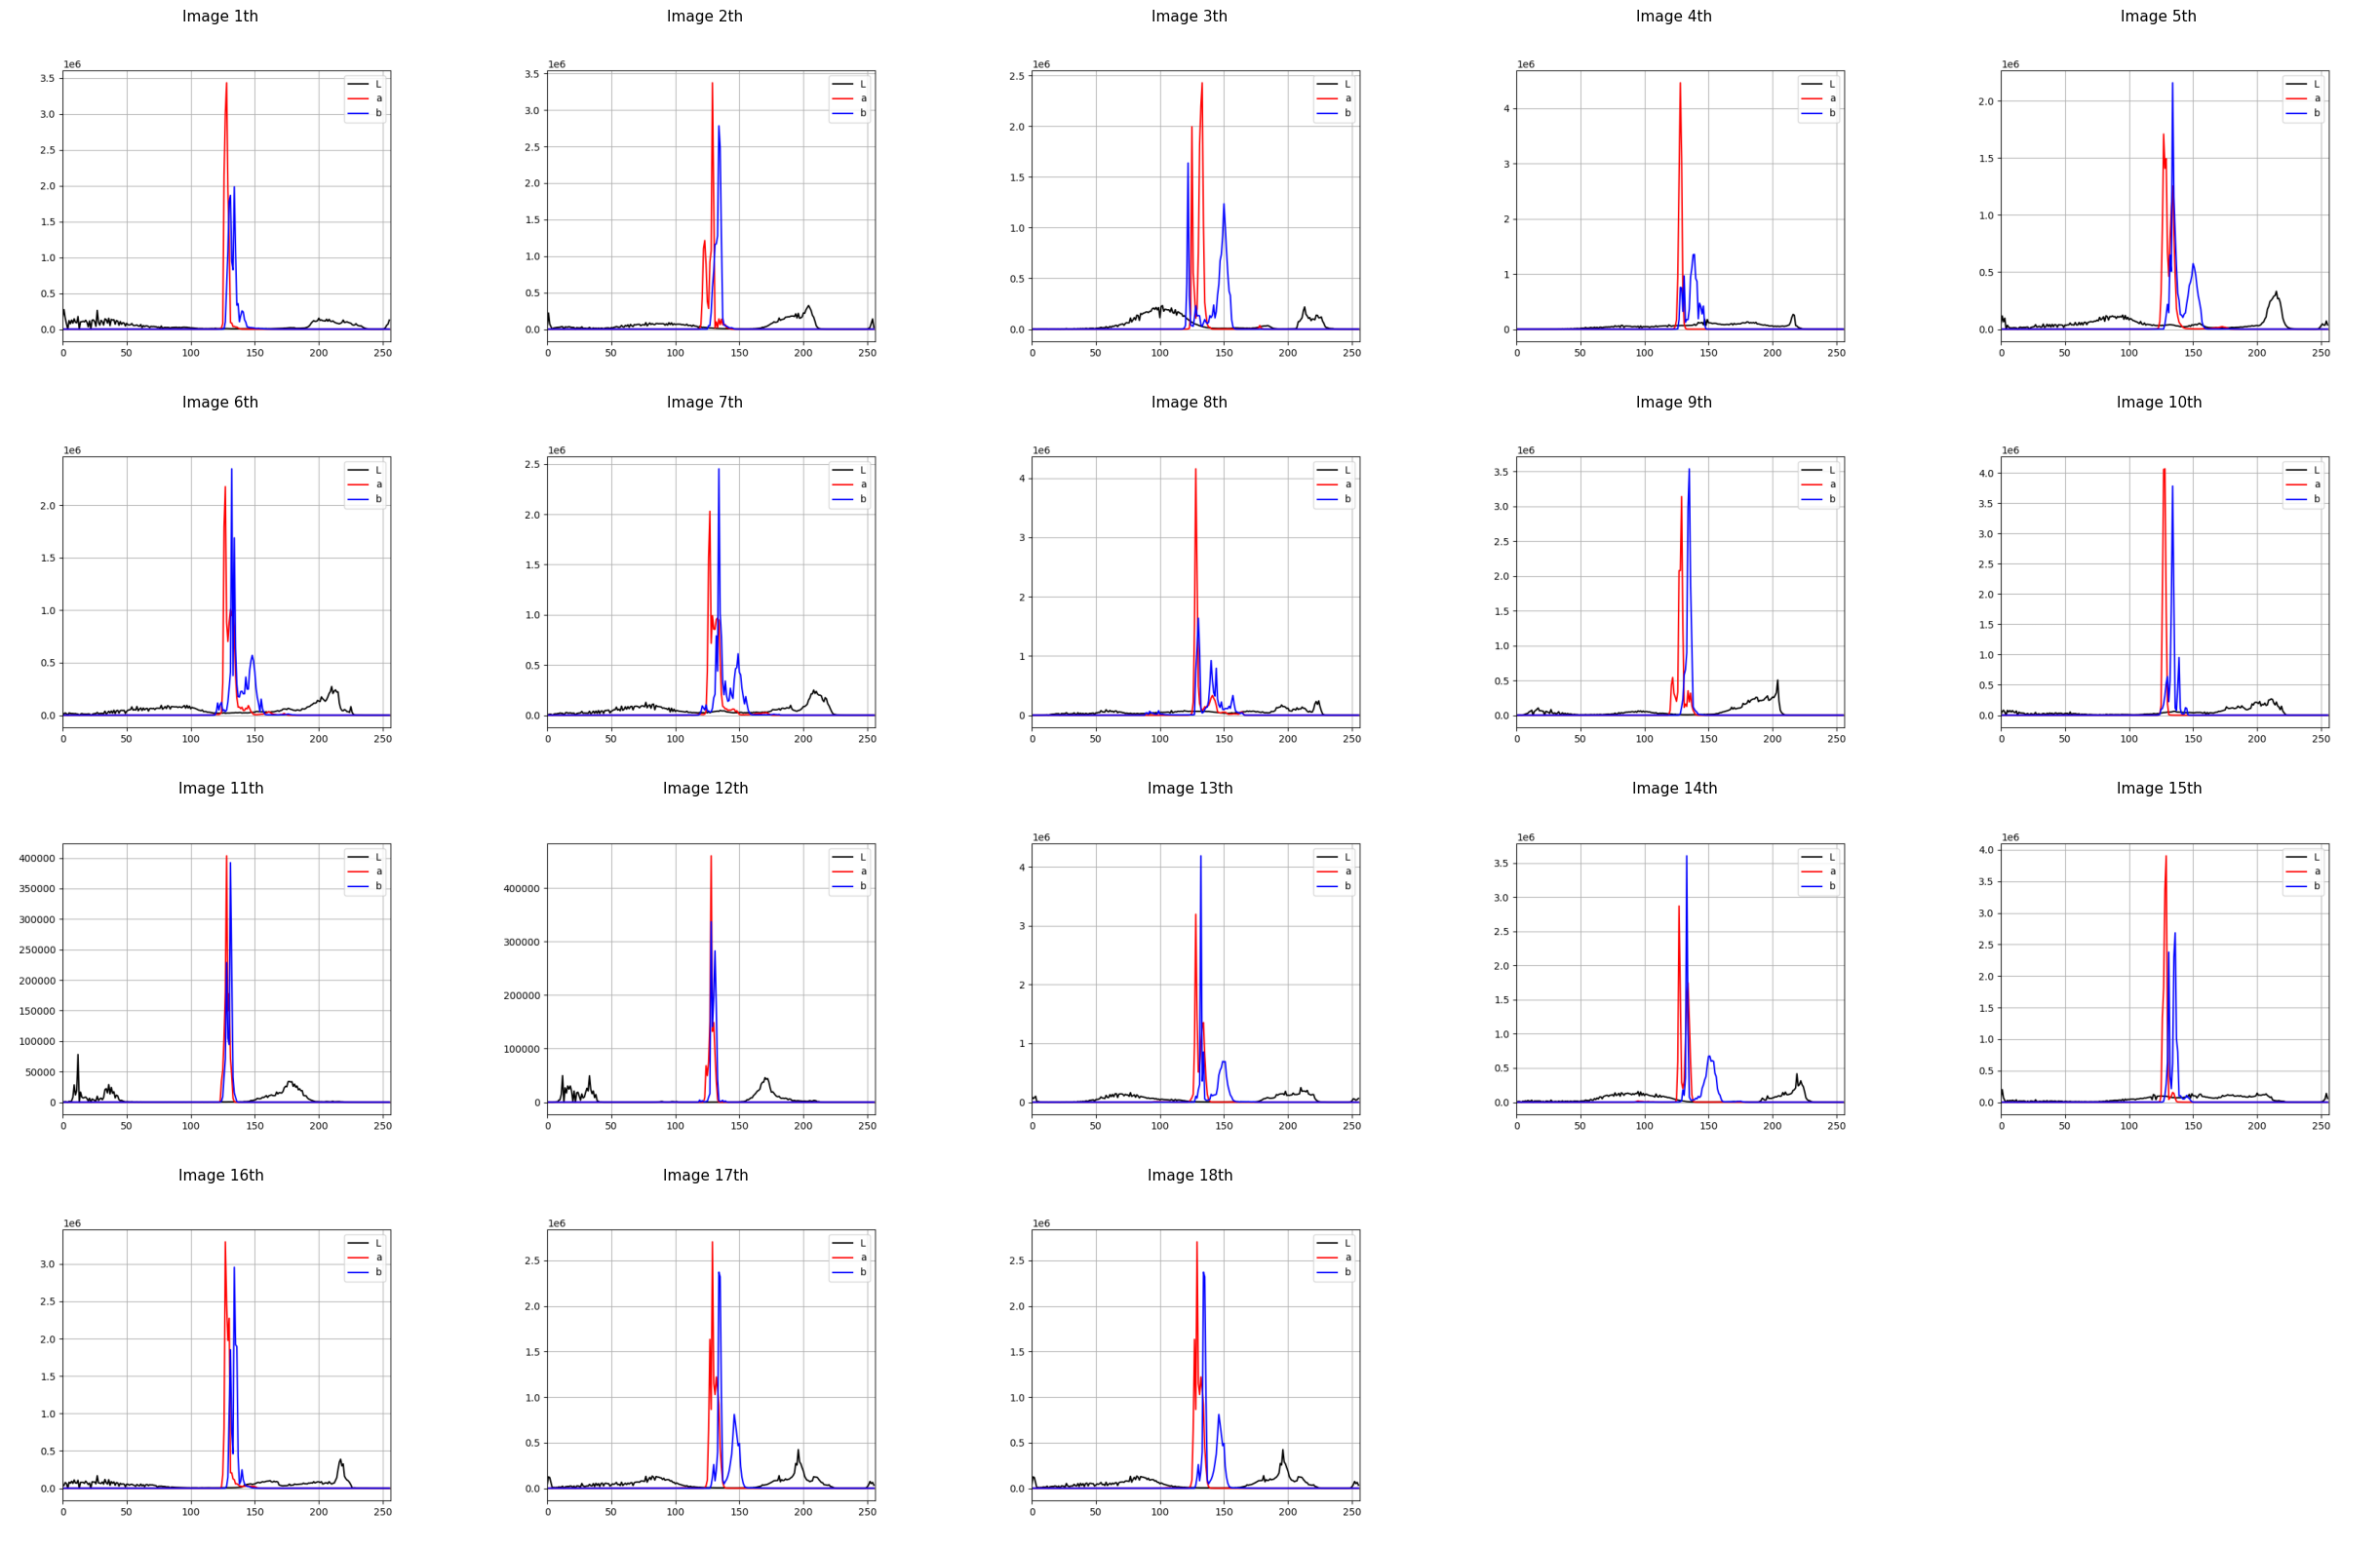
\includegraphics[width=0.9\textwidth]{hist_lab.png}
\caption{Histogram của một số ảnh trong hệ màu LAB}
\end{figure}

Trong không gian màu LAB, kênh L thể hiện độ sáng của ảnh. Histogram kênh L thường trải rộng và có nhiều đỉnh, cho thấy ảnh có sự thay đổi mạnh về ánh sáng giữa vùng giấy, nền bàn, sàn và bóng đổ.

Hai kênh A và B có đỉnh rất cao, hẹp và tập trung quanh vùng giữa khoảng 120–140. Điều này cho thấy phần lớn ảnh có màu gần trung tính, phù hợp với ảnh tài liệu gồm giấy trắng, chữ đen và nền ít màu.

Ở một số ảnh, kênh A hoặc B bị lệch nhẹ, cho thấy ảnh có hiện tượng ám màu do ánh sáng môi trường, ví dụ ánh sáng vàng, xanh hoặc phản xạ từ nền xung quanh.


\section{Kết quả tiền xử lý ảnh}

\subsection{So sánh các phương pháp làm mờ}

Hai phương pháp làm mờ được sử dụng bao gồm Gaussian Blur và Median Blur.

\begin{figure}[H]
\centering

\begin{subfigure}{0.48\textwidth}
    \centering
    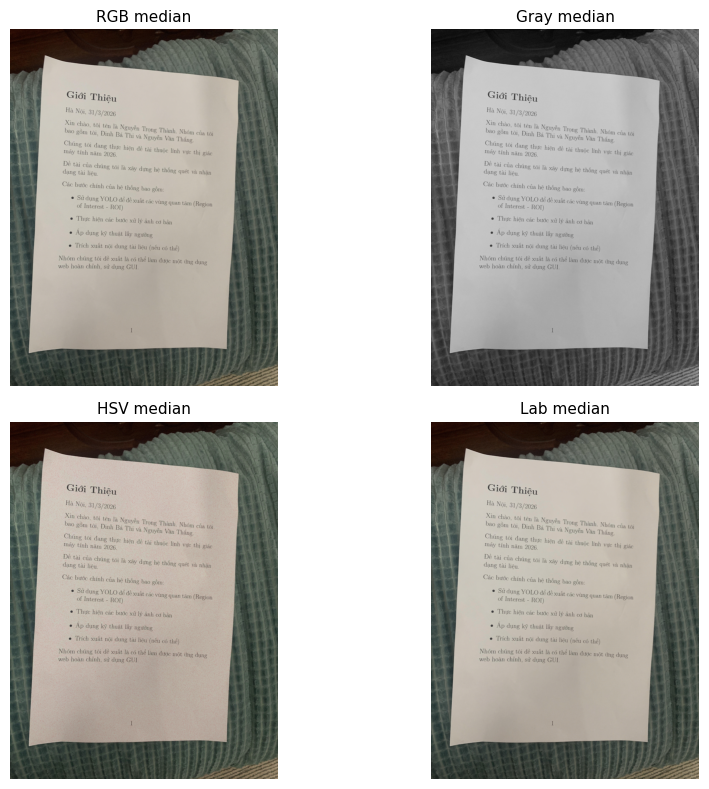
\includegraphics[width=\textwidth]{median_after.png}
    \caption{Kết quả sau Median Blur}
\end{subfigure}
\hfill
\begin{subfigure}{0.48\textwidth}
    \centering
    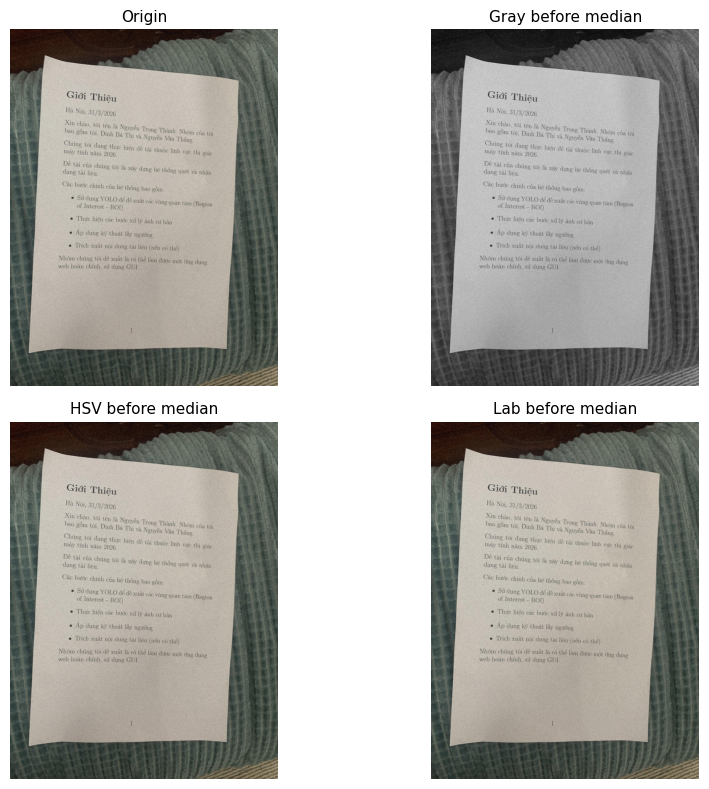
\includegraphics[width=\textwidth]{median_before.png}
    \caption{Ảnh trước Median Blur}
\end{subfigure}

\vspace{0.4cm}

\begin{subfigure}{0.48\textwidth}
    \centering
    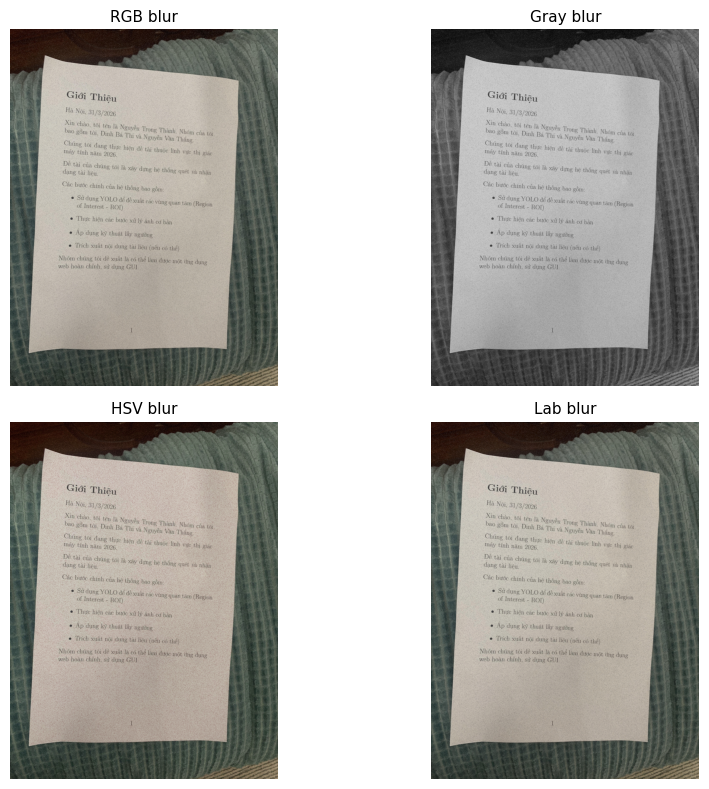
\includegraphics[width=\textwidth]{gaussian_after.png}
    \caption{Kết quả sau Gaussian Blur}
\end{subfigure}
\hfill
\begin{subfigure}{0.48\textwidth}
    \centering
    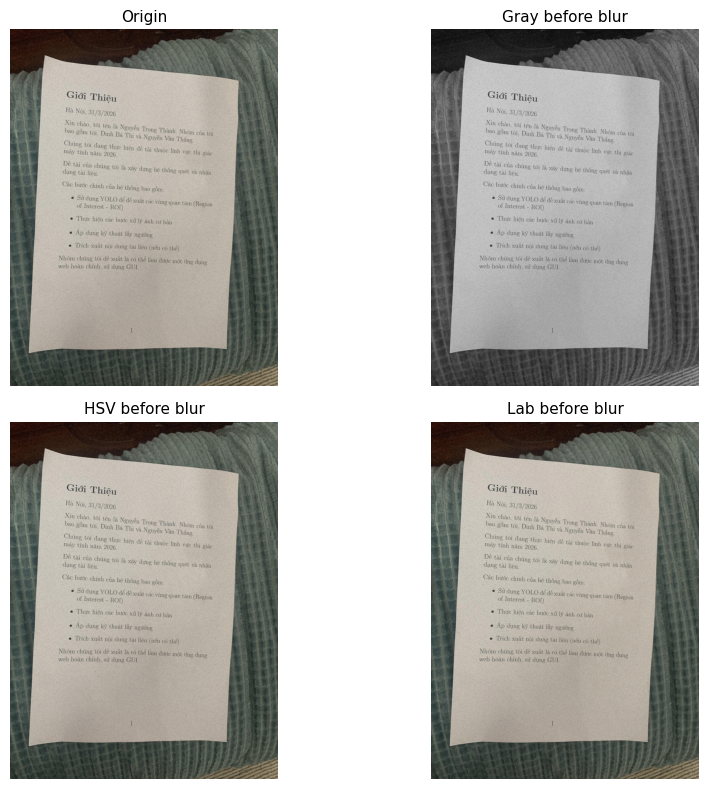
\includegraphics[width=\textwidth]{gaussian_before.png}
    \caption{Ảnh trước Gaussian Blur}
\end{subfigure}

\caption{So sánh ảnh trước và sau khi áp dụng các phương pháp làm mờ}
\end{figure}


\textbf{Nhận xét:}
\begin{itemize}
    \item Gaussian Blur làm mượt ảnh tự nhiên nhưng dễ làm mờ và mất các biên giấy mảnh.
    \item Median Blur giữ cạnh biên tốt hơn và loại bỏ cực kỳ hiệu quả các hạt nhiễu tiêu (Salt \& Pepper).
\end{itemize}

\subsection{Làm sắc nét ảnh}
Trong bài toán scan tài liệu, Median Blur được dùng để giảm nhiễu nhỏ trên nền giấy và vùng xung quanh tài liệu. Phương pháp này làm mịn ảnh nhưng vẫn giữ tương đối tốt các cạnh quan trọng như biên tờ giấy và nét chữ.

Sau khi làm mịn, ảnh có thể bị giảm độ sắc nét nhẹ. Vì vậy, bước làm sắc nét được áp dụng để tăng cường các vùng chuyển tiếp cường độ, đặc biệt tại mép giấy và vùng chữ. Quá trình này sử dụng hạt nhân $3 \times 3$:

\[
K_{sharpen} =
\begin{bmatrix}
0 & -1 & 0 \\
-1 & 5 & -1 \\
0 & -1 & 0
\end{bmatrix}
\]

Hạt nhân trên giúp nhấn mạnh điểm ảnh trung tâm và giảm ảnh hưởng từ các điểm lân cận, nhờ đó biên ảnh rõ hơn. Kết quả này hỗ trợ tốt cho các bước phát hiện biên như Canny hoặc Sobel.

Ví dụ:


\begin{figure}[H]
\centering

\begin{subfigure}{0.48\textwidth}
    \centering
    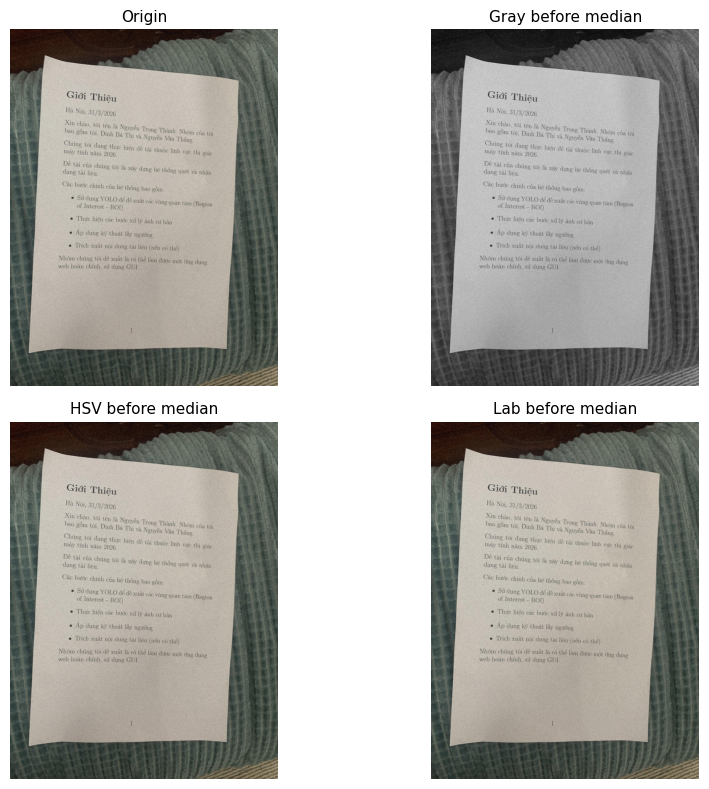
\includegraphics[width=\textwidth]{median_before.png}
    \caption{Kết quả trước khi làm sắc ảnh}
\end{subfigure}
\hfill
\begin{subfigure}{0.48\textwidth}
    \centering
    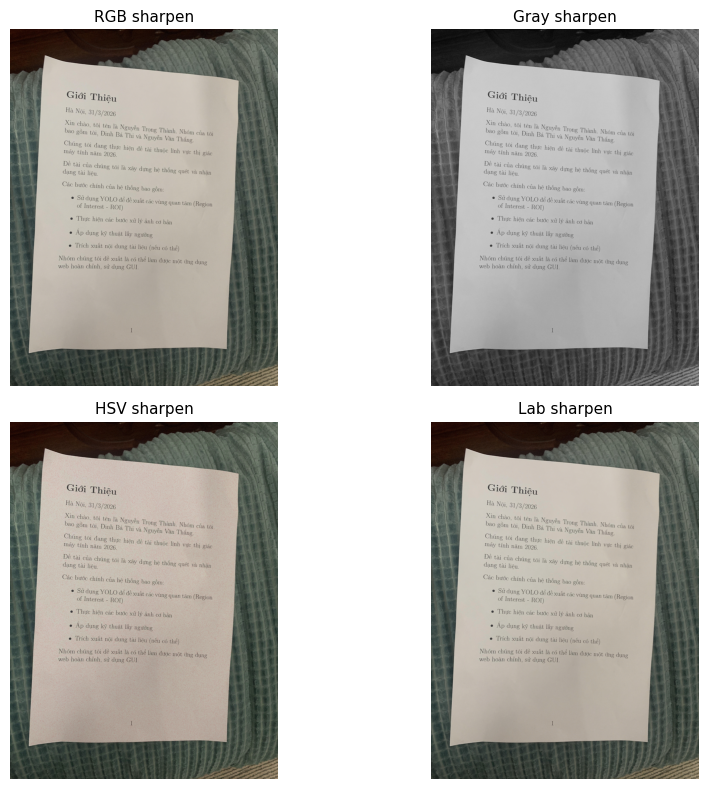
\includegraphics[width=\textwidth]{sample_sharpen.png}
    \caption{Kết quả sau khi làm sắc ảnh}
\end{subfigure}

\caption{Ví dụ trước và sau khi làm sắc ảnh}
\end{figure}

\textbf{Nhận xét:}

Qua thực nghiệm, các phương pháp sharpen đều giúp làm rõ biên giấy và nét chữ. RGB giữ màu tốt nhưng dễ làm tăng nhiễu nền. Gray phù hợp cho threshold và phát hiện biên. HSV và LAB cho kết quả ổn định hơn, trong đó LAB sharpen thường cân bằng tốt giữa độ rõ, độ tự nhiên và khả năng giảm ảnh hưởng của màu nền.



\subsection{Cân bằng sáng}

Trong lần thực nghiệm này, chúng tôi sử dụng cân bằng sáng nhằm cải thiện độ tương phản và làm rõ nội dung tài liệu. Do ảnh đầu vào được chụp trong nhiều điều kiện ánh sáng khác nhau, ảnh có thể bị tối, cháy sáng hoặc xuất hiện bóng đổ, gây khó khăn cho quá trình phát hiện biên và tìm contour.

Các phương pháp được thử nghiệm gồm Histogram Equalization (HE) và CLAHE trên các không gian màu Gray, HSV và LAB. HE giúp tăng tương phản toàn cục, trong khi CLAHE tăng tương phản cục bộ và thường ổn định hơn với ảnh có ánh sáng không đồng đều.

\begin{figure}[H]
\centering
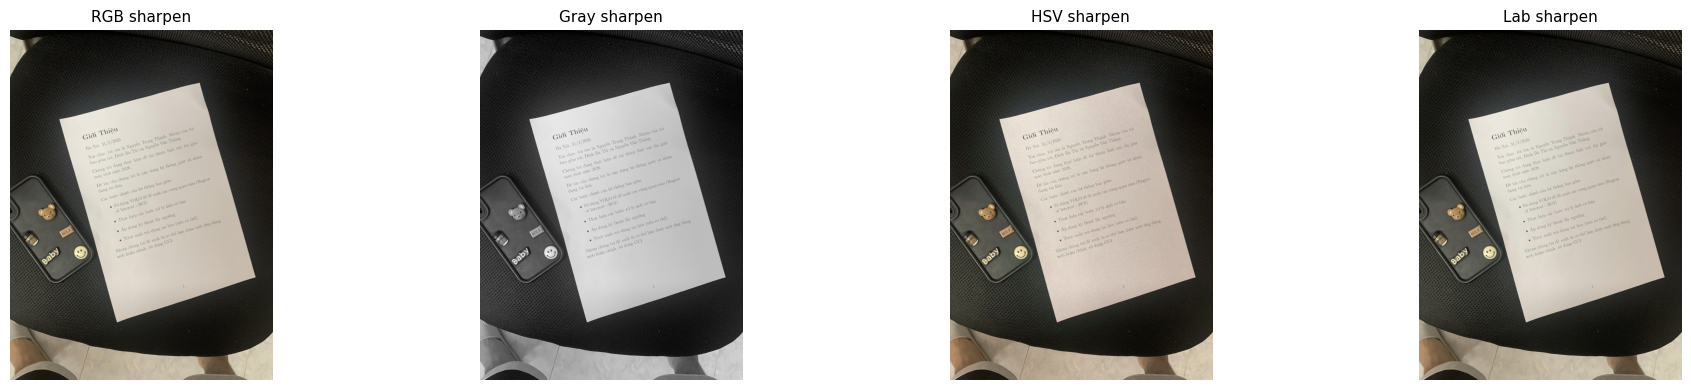
\includegraphics[width=0.95\textwidth]{eq1.png}
\caption{So sánh kết quả Histogram Equalization và CLAHE trên các không gian màu đối với ảnh mẫu thứ nhất}
\end{figure}

\begin{figure}[H]
\centering
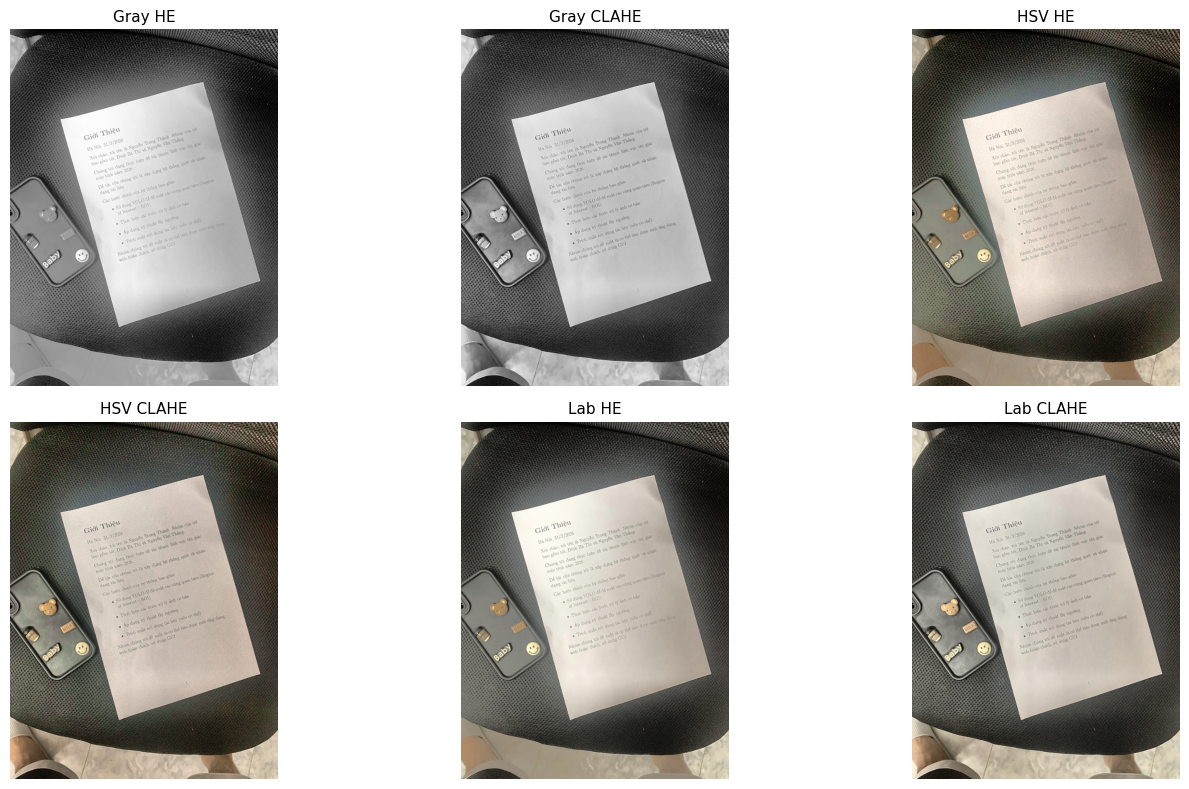
\includegraphics[width=0.95\textwidth]{eq1_op.png}
\caption{So sánh kết quả làm sắc nét ảnh trên các không gian màu đối với ảnh mẫu thứ nhất}
\end{figure}

\begin{figure}[H]
\centering
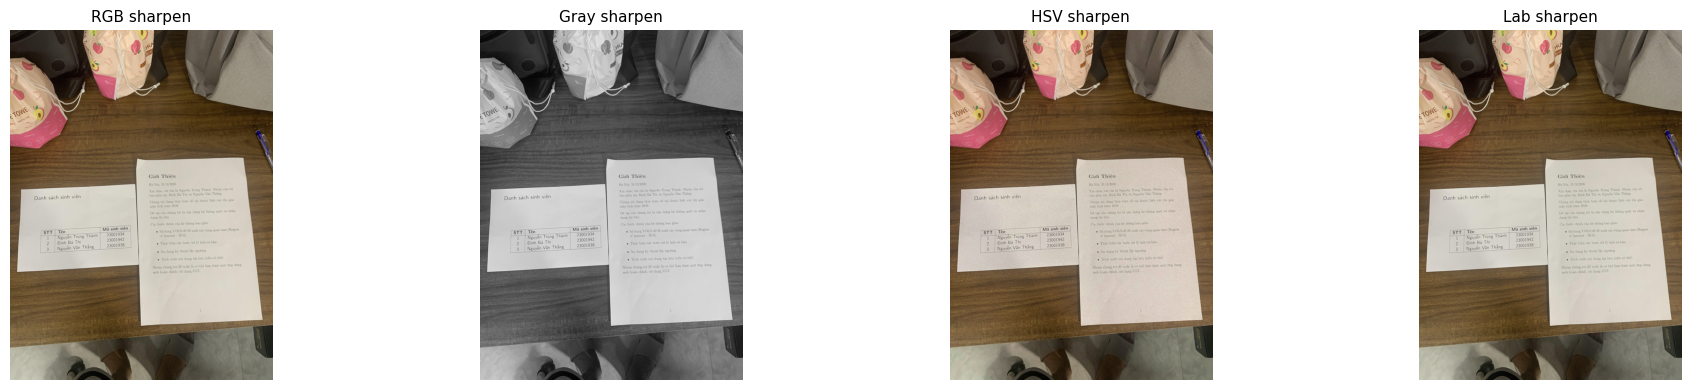
\includegraphics[width=0.95\textwidth]{eq2.png}
\caption{So sánh kết quả Histogram Equalization và CLAHE trên các không gian màu đối với ảnh mẫu thứ hai}
\end{figure}

\begin{figure}[H]
\centering
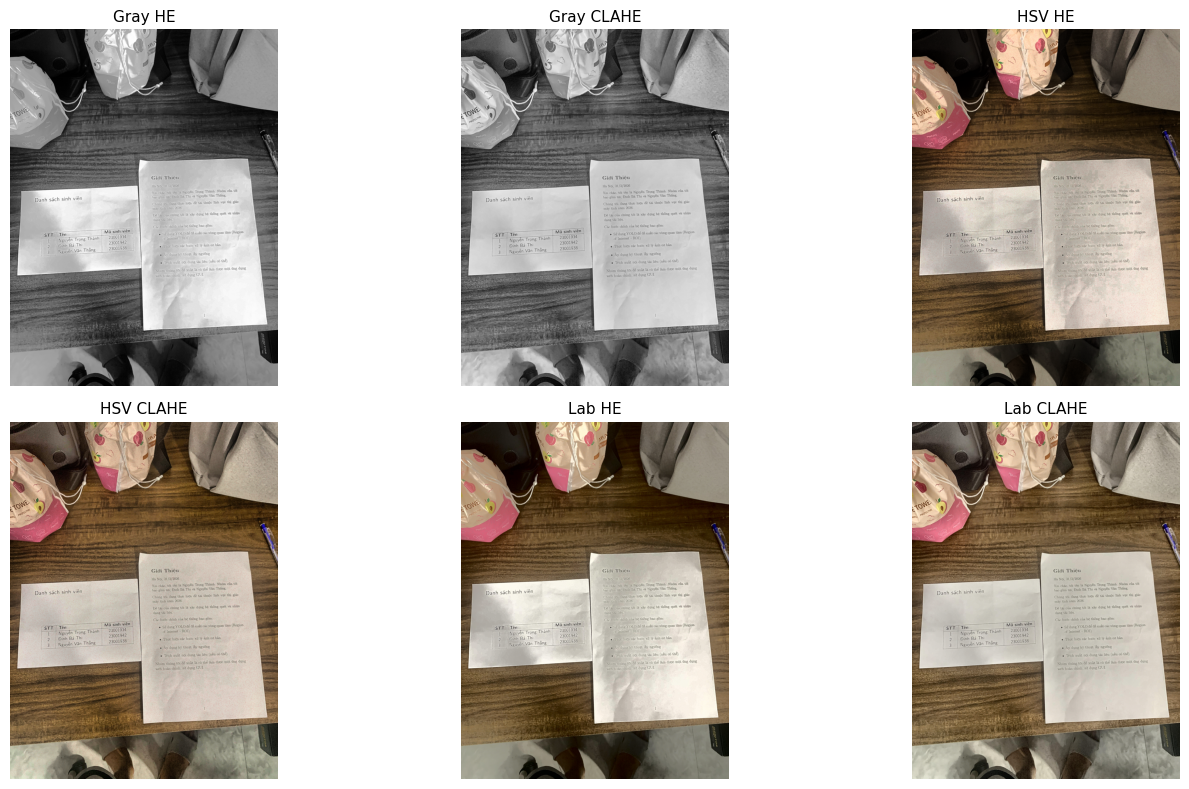
\includegraphics[width=0.95\textwidth]{eq2_op.png}
\caption{So sánh kết quả làm sắc nét ảnh trên các không gian màu đối với ảnh mẫu thứ hai}
\end{figure}


\begin{figure}[H]
\centering
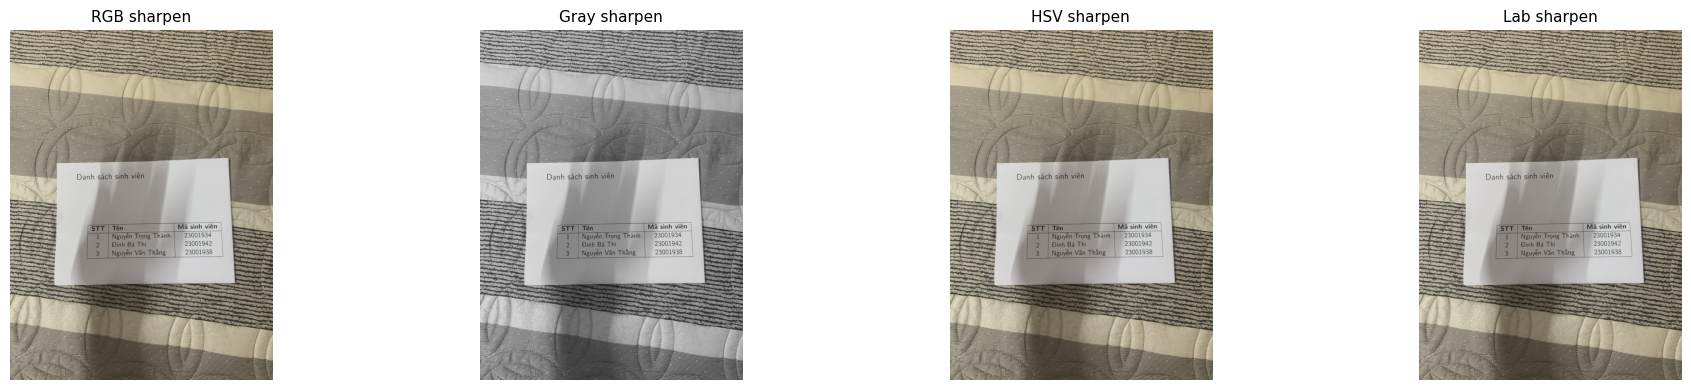
\includegraphics[width=0.95\textwidth]{eq3.png}
\caption{So sánh kết quả Histogram Equalization và CLAHE trên các không gian màu đối với ảnh mẫu thứ ba}
\end{figure}

\begin{figure}[H]
\centering
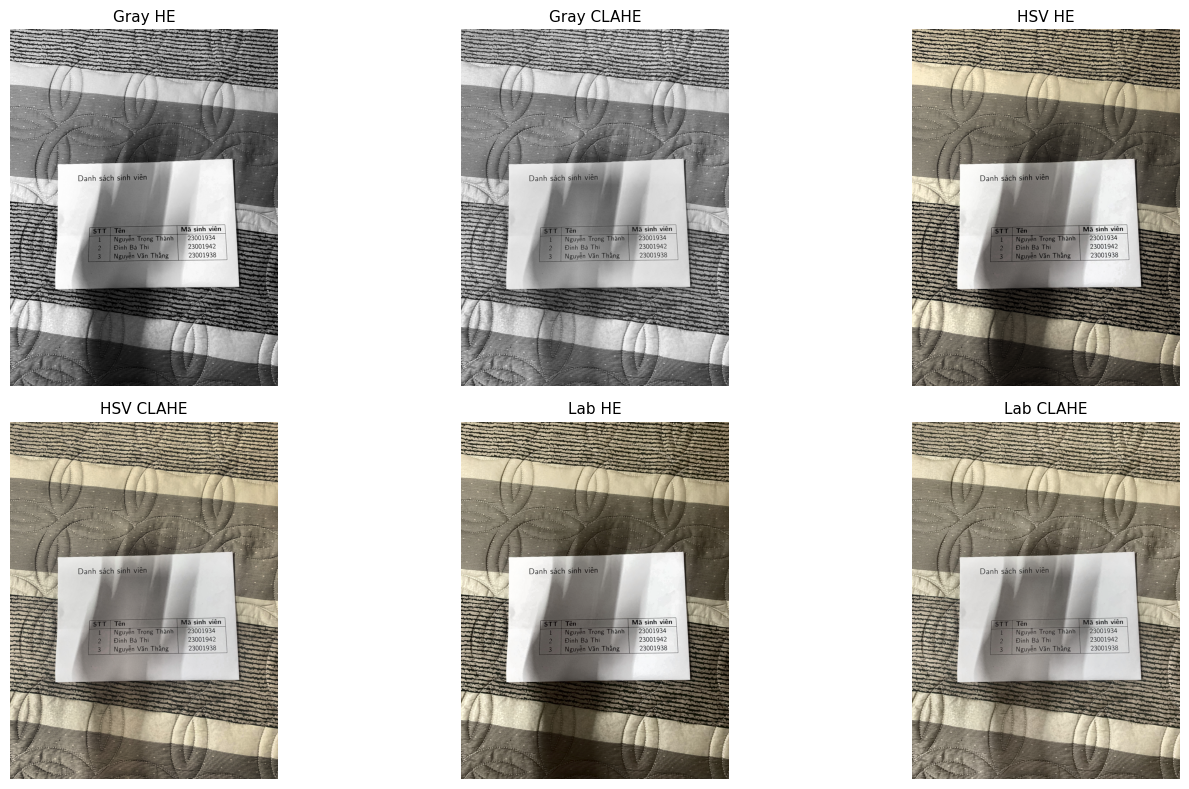
\includegraphics[width=0.95\textwidth]{eq3_op.png}
\caption{So sánh kết quả làm sắc nét ảnh trên các không gian màu đối với ảnh mẫu thứ ba}
\end{figure}

\textbf{Nhận xét:}

Qua thực nghiệm, các phương pháp cân bằng sáng giúp cải thiện độ tương phản, làm rõ vùng giấy và nội dung chữ. HE tăng tương phản mạnh nhưng dễ làm ảnh bị gắt, đồng thời khuếch đại nhiễu và bóng đổ.

CLAHE cho kết quả ổn định hơn, đặc biệt với ảnh có ánh sáng không đồng đều. Trong các không gian màu thử nghiệm, Gray phù hợp cho threshold và phát hiện biên, còn LAB cho kết quả tự nhiên, cân bằng hơn. CLAHE trên Gray hoặc LAB là lựa chọn phù hợp hơn cho bài toán scan tài liệu.


% \subsection{Biến đổi hình thái}

% \begin{figure}[H]
% \centering
% \includegraphics[width=\textwidth]{morphology.png}
% \caption{Kết quả các phép biến đổi hình thái}
% \end{figure}

% \textbf{Nhận xét:}
% \begin{itemize}
%     \item Phép Mở (Opening) kết hợp chuỗi Erosion tiếp nối bởi Dilation, đóng vai trò như bộ lọc vật lý giúp dập tắt hoàn toàn các chấm nhiễu rác li ti sinh ra từ vân gỗ hoặc nhiễu tiêu.
%     \item Closing giúp lấp đầy các khoảng trống bên trong vùng văn bản do lỗi phản quang.
% \end{itemize}

\section{Phát hiện biên}

Hệ thống xem xét cả thuật toán Canny truyền thống và Sobel kết hợp với Thresholding.

\subsection{Sobel và Thresholding}

\subsubsection{Trên ảnh xám}

\begin{figure}[H]
\centering
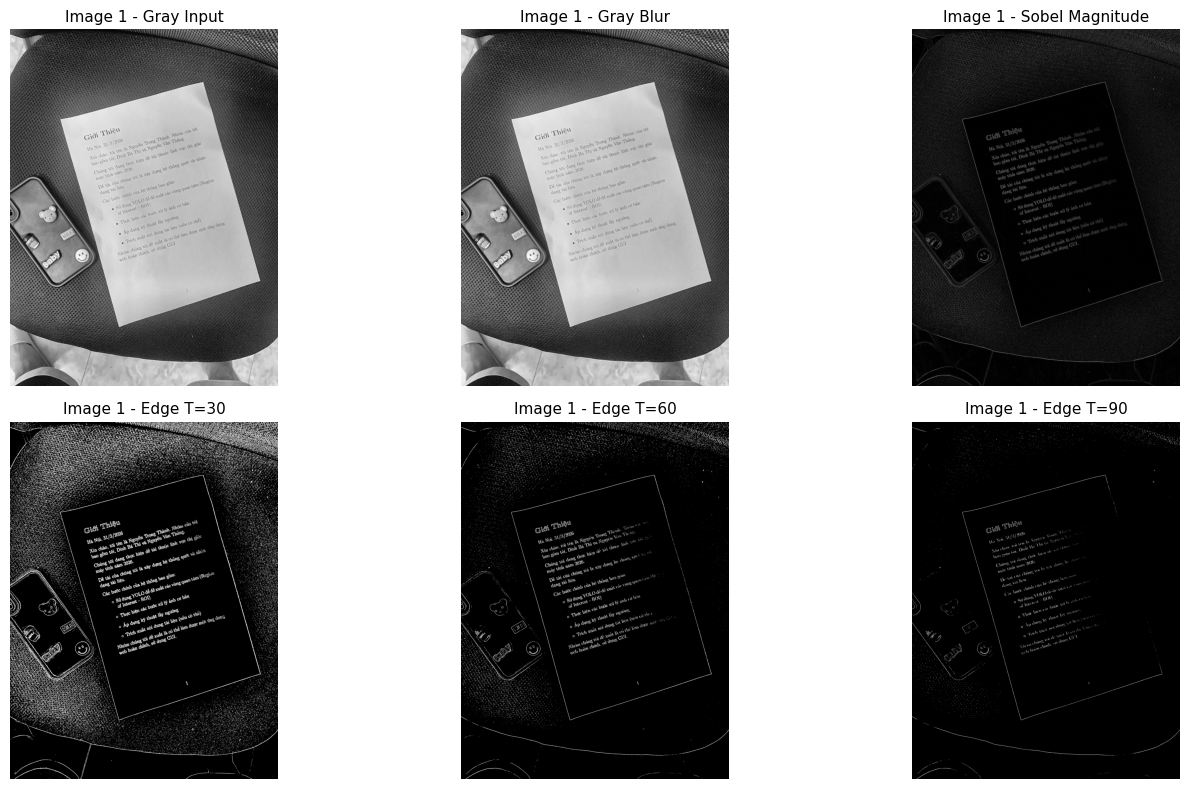
\includegraphics[width=0.95\textwidth]{edge1.1.png}
\caption{Kết quả phát hiện biên Sobel + Thresholding trên ảnh mẫu thứ nhất}
\end{figure}

% \begin{figure}[H]
% \centering
% 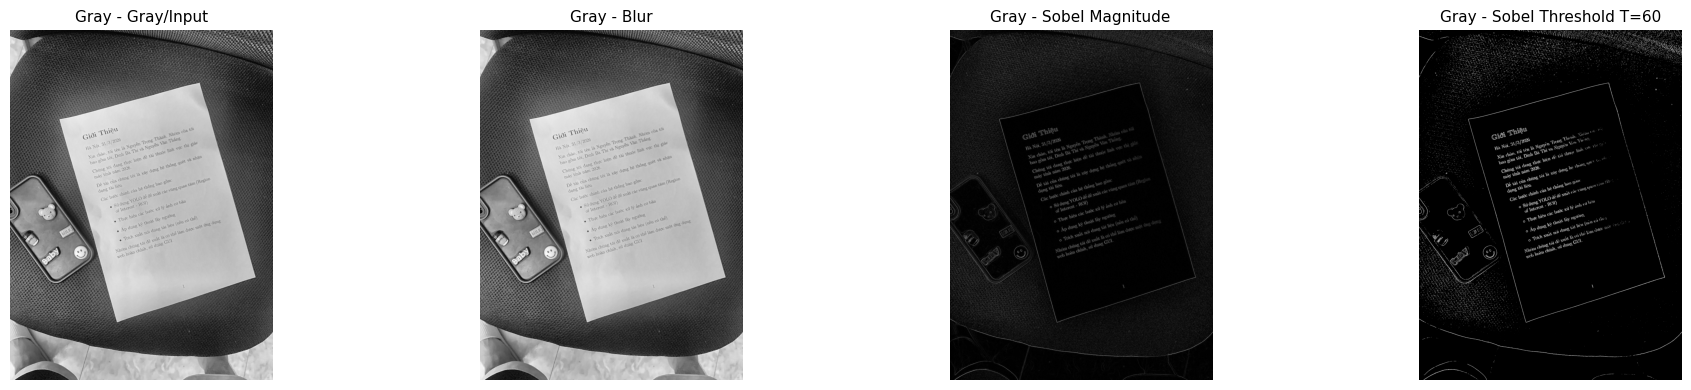
\includegraphics[width=0.95\textwidth]{edge1_60.png}
% \caption{Kết quả phát hiện biên Sobel trên ảnh mẫu thứ nhất với ngưỡng $T=60$}
% \end{figure}

% \begin{figure}[H]
% \centering
% 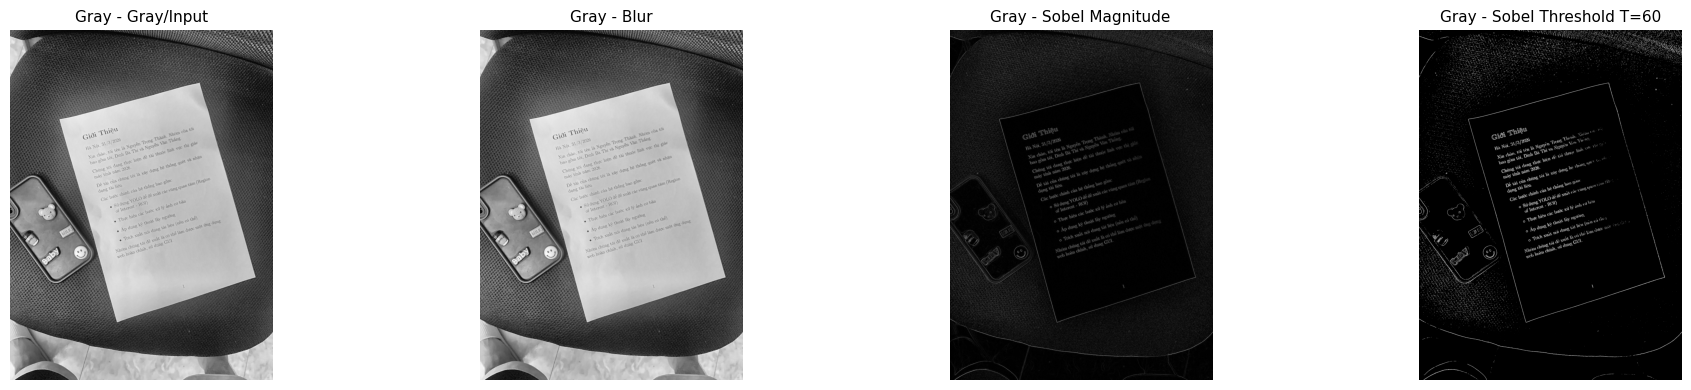
\includegraphics[width=0.95\textwidth]{edge1_90.png}
% \caption{Kết quả phát hiện biên Sobel trên ảnh mẫu thứ nhất với ngưỡng $T=90$}
% \end{figure}

\vspace{0.4cm}

\begin{figure}[H]
\centering
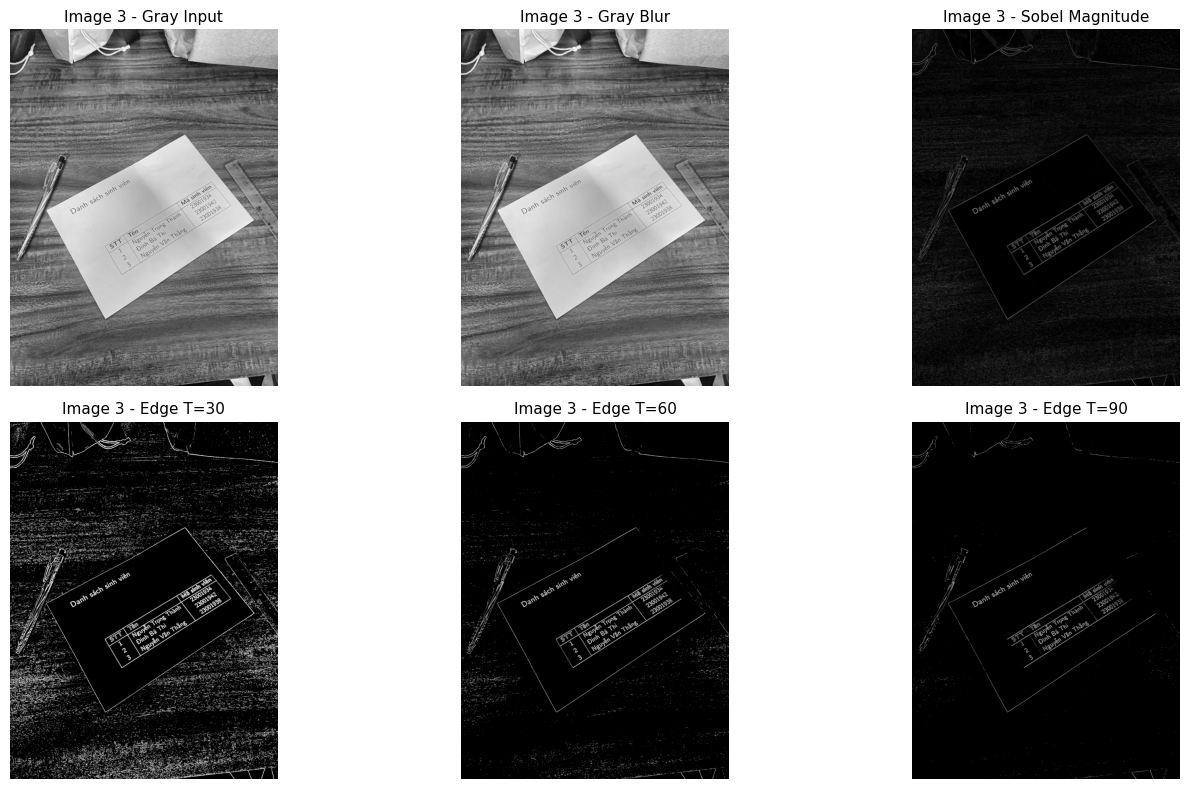
\includegraphics[width=0.95\textwidth]{edge2.1.png}
\caption{Kết quả phát hiện biên Sobel + Thresholding trên ảnh mẫu thứ hai}
\end{figure}

% \begin{figure}[H]
% \centering
% 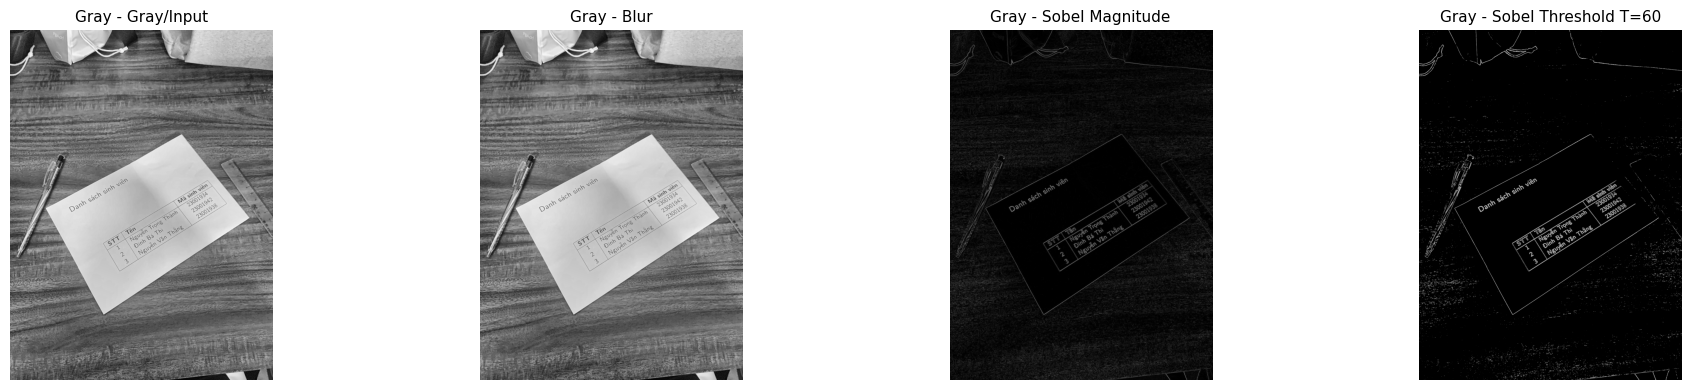
\includegraphics[width=0.95\textwidth]{edge2_60.png}
% \caption{Kết quả phát hiện biên Sobel trên ảnh mẫu thứ hai với ngưỡng $T=60$}
% \end{figure}

% \begin{figure}[H]
% \centering
% 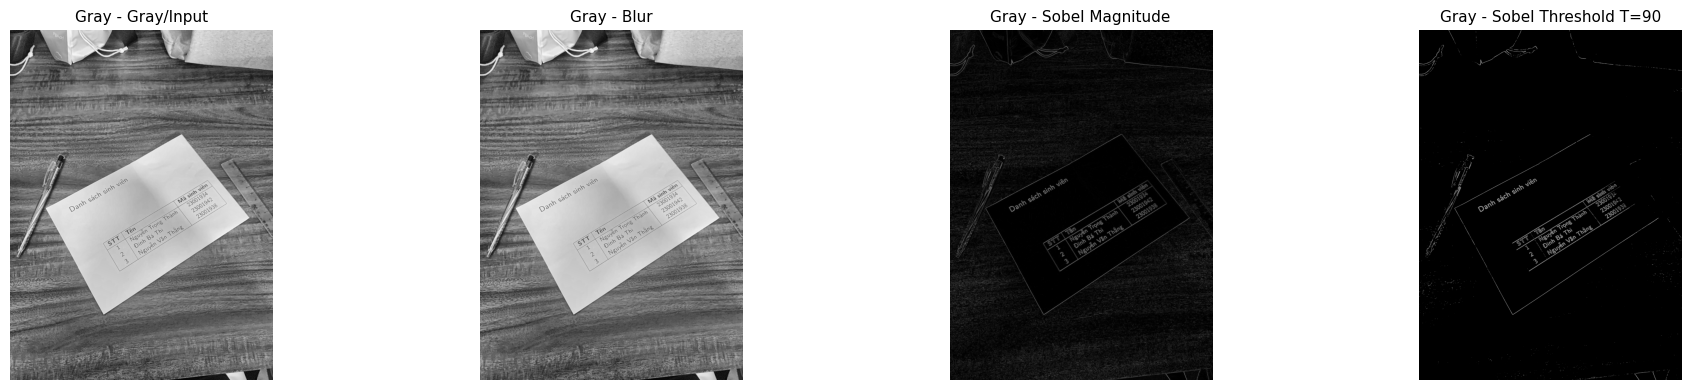
\includegraphics[width=0.95\textwidth]{edge2_90.png}
% \caption{Kết quả phát hiện biên Sobel trên ảnh mẫu thứ hai với ngưỡng $T=90$}
% \end{figure}

Qua trực quan, ngưỡng $T$ ảnh hưởng lớn đến chất lượng biên thu được. Với $T=30$, nhiều chi tiết nền và nhiễu cũng được giữ lại, làm ảnh biên rối và khó tìm contour chính xác. Với $T=90$, biên trở nên sạch hơn nhưng một số đoạn biên của tài liệu có thể bị mất hoặc đứt gãy. Ngưỡng $T=60$ cho kết quả cân bằng hơn, giữ được biên giấy tương đối rõ trong khi vẫn hạn chế bớt nhiễu nền.

% \subsubsection{Hệ màu HSV}

% Thay vì chỉ áp dụng trên một kênh mức xám, hệ thống thử nghiệm chuyển đổi ảnh sang không gian màu HSV. Toán tử Sobel được áp dụng độc lập trên từng kênh: Hue (Màu sắc), Saturation (Độ bão hòa) và Value (Độ sáng). Sau đó, độ lớn gradient của cả ba kênh được tổng hợp lại (Merged Magnitude) và đi qua bước phân ngưỡng (Thresholding) để tạo ra ảnh biên cuối cùng (Final Edge). Thực nghiệm được đánh giá qua các ngưỡng $T$ lần lượt là 30, 60 và 90.

% \begin{figure}[H]
% \centering
% 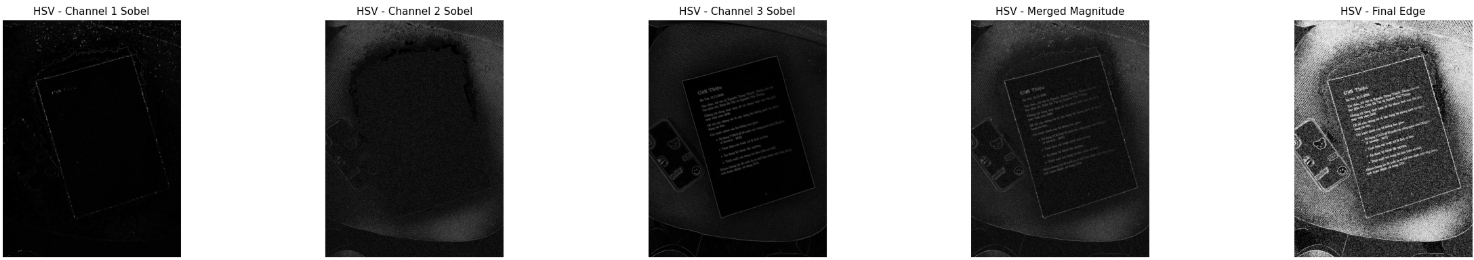
\includegraphics[width=\textwidth]{sobel_hsv_t30.png}
% \caption{Quá trình phát hiện biên Sobel trên hệ màu HSV với ngưỡng $T=30$}
% \end{figure}

% \begin{figure}[H]
% \centering
% 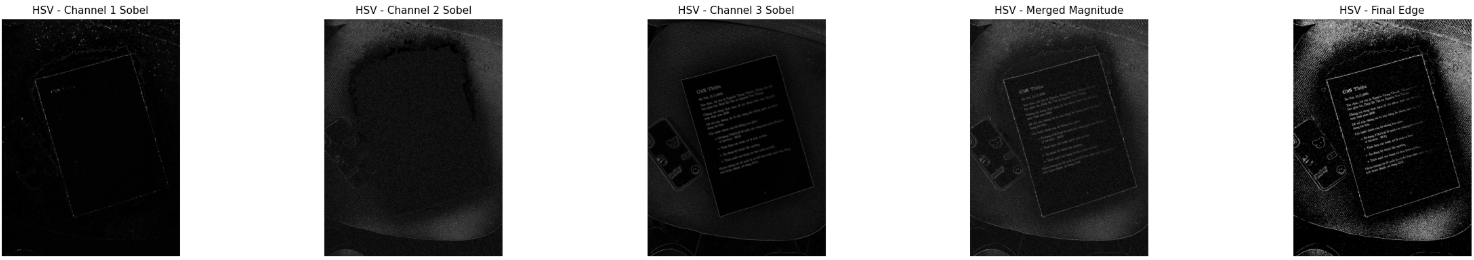
\includegraphics[width=\textwidth]{sobel_hsv_t60.png}
% \caption{Quá trình phát hiện biên Sobel trên hệ màu HSV với ngưỡng $T=60$}
% \end{figure}

% \begin{figure}[H]
% \centering
% 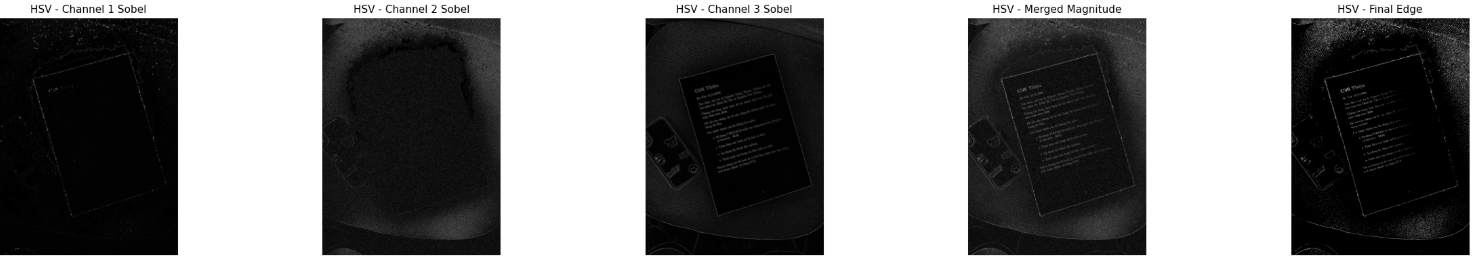
\includegraphics[width=\textwidth]{sobel_hsv_t90.png}
% \caption{Quá trình phát hiện biên Sobel trên hệ màu HSV với ngưỡng $T=90$}
% \end{figure}

% \textbf{Nhận xét thực nghiệm:}

% \begin{itemize}
%     \item \textbf{Đánh giá từng kênh:} Kênh V (Độ sáng) nhận diện ranh giới giấy rất tốt. Ngược lại, kênh H (Màu sắc) và S (Độ bão hòa) quá nhạy cảm với màu sắc và bóng đổ, kéo theo lượng lớn nhiễu từ cấu trúc nền.
%     \item \textbf{Tác động của ngưỡng $T$:} Ở mức $T=30$, nhiễu từ kênh H và S cộng hưởng làm chìm nghỉm biên tài liệu. Dù tăng ngưỡng lên $60$ hay $90$, ảnh biên tổng hợp vẫn chứa quá nhiều rác nét vụn nếu so sánh với phương pháp xử lý trên ảnh xám (Gray).
% \end{itemize}

% \textbf{Kết luận:} Việc gộp gradient 3 kênh HSV để dò biên không hiệu quả trên nền họa tiết phức tạp. Thông tin biến thiên màu sắc thừa thãi từ kênh H và S tạo ra lượng nhiễu khổng lồ, phá hỏng mask định vị tài liệu.

% \subsubsection{Hệ màu LAB}

% Tiếp tục hành trình khảo sát, hệ thống thực hiện phát hiện biên Sobel trên không gian màu CIELAB (LAB). Không gian này có đặc tính ưu việt là tách biệt hoàn toàn kênh độ sáng (L - Lightness) khỏi các kênh màu sắc (A và B). Tương tự như HSV, độ lớn gradient của cả ba kênh được tổng hợp lại và áp dụng phân ngưỡng tại các mức $T = 30, 60, 90$.

% \begin{figure}[H]
% \centering
% 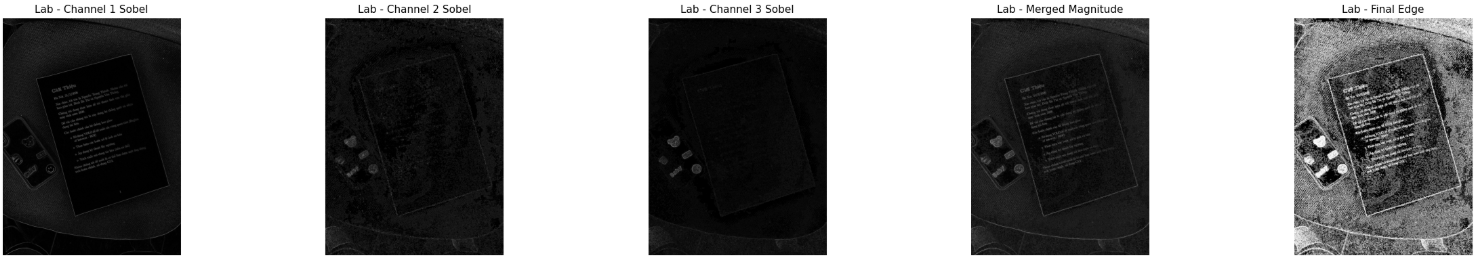
\includegraphics[width=\textwidth]{sobel_lab_t30.png}
% \caption{Quá trình phát hiện biên Sobel trên hệ màu LAB với ngưỡng $T=30$}
% \end{figure}

% \begin{figure}[H]
% \centering
% 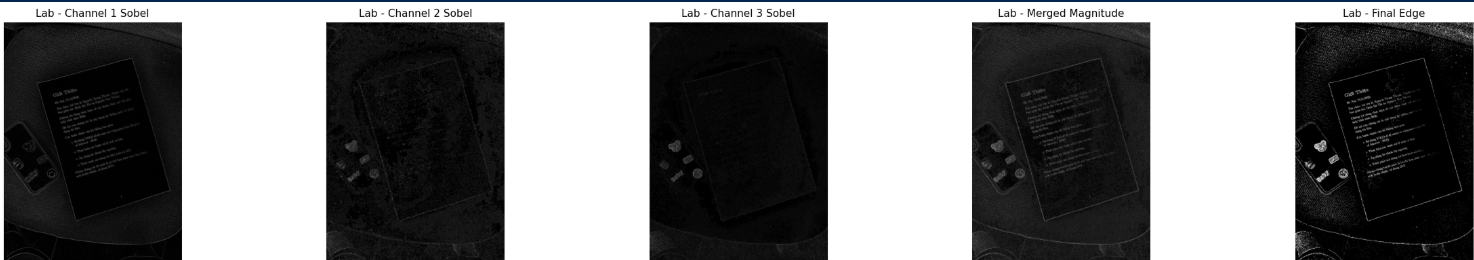
\includegraphics[width=\textwidth]{sobel_lab_t60.png}
% \caption{Quá trình phát hiện biên Sobel trên hệ màu LAB với ngưỡng $T=60$}
% \end{figure}

% \begin{figure}[H]
% \centering
% 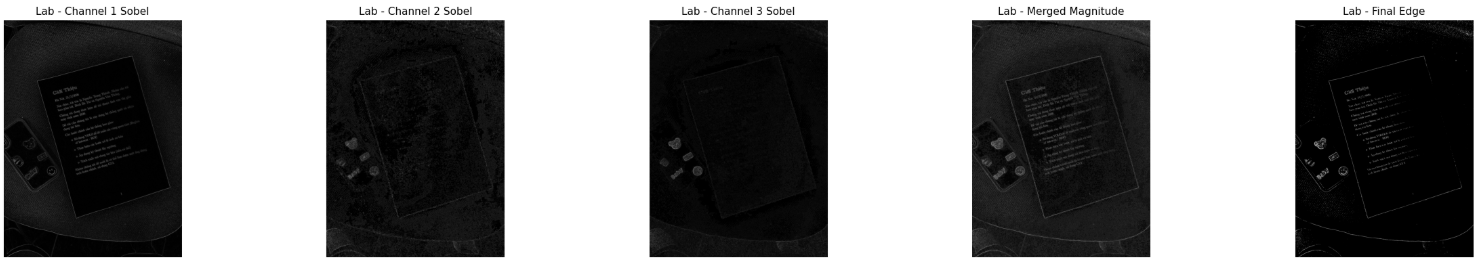
\includegraphics[width=\textwidth]{sobel_lab_t90.png}
% \caption{Quá trình phát hiện biên Sobel trên hệ màu LAB với ngưỡng $T=90$}
% \end{figure}

% \textbf{Nhận xét thực nghiệm:}

% \begin{itemize}
%     \item \textbf{Đánh giá từng kênh:} Kênh L (Lightness) cô lập độ sáng cực tốt, làm nổi bật rõ ranh giới giấy và chữ. Ngược lại, hai kênh A và B (Màu sắc) gần như không tạo ra đường biên hữu ích do bản chất giấy màu trắng, thậm chí còn kéo theo nhiễu màu từ môi trường.
%     \item \textbf{Tác động của gộp kênh và ngưỡng $T$:} Ảnh gộp (Merged Magnitude) ở ngưỡng thấp ($T=30$) vẫn bị nhiễu chi tiết nền. Khi tăng ngưỡng ($T=60, 90$), viền tài liệu trở nên sắc nét, ít đứt gãy và "sạch" hơn hẳn so với hệ HSV.
% \end{itemize}

% \textbf{Kết luận:} Hệ LAB cho kết quả tốt nhờ khả năng tách biệt ánh sáng. Tuy nhiên, việc cộng gộp kênh $A$ và $B$ là thao tác dư thừa, làm tăng nhiễu không đáng có. Do đó, giải pháp tối ưu nhất là \textbf{chỉ trích xuất kênh L} kết hợp với các bộ lọc hình thái học để dò tìm biên tài liệu.

\subsubsection{Hệ màu RGB}

Thực nghiệm tiếp theo được tiến hành trên không gian màu gốc RGB. Toán tử Sobel được áp dụng độc lập trên ba kênh Đỏ (R), Lục (G), Lam (B). Sau đó, các dải gradient được gộp lại (Merged Magnitude) và phân ngưỡng tại các mức $T = 30, 60, 90$.

\begin{figure}[H]
\centering
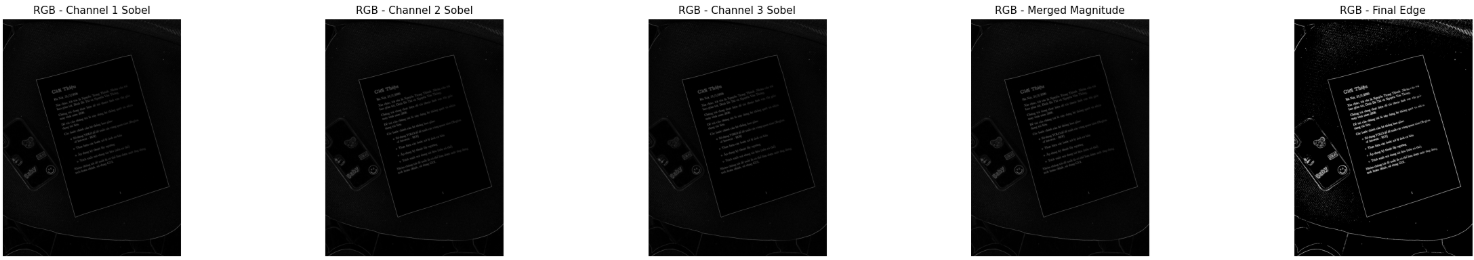
\includegraphics[width=\textwidth]{sobel_rgb_t30.png}
\caption{Quá trình phát hiện biên  Sobel + Thresholding trên hệ màu RGB với ngưỡng $T=30$}
\end{figure}

\begin{figure}[H]
\centering
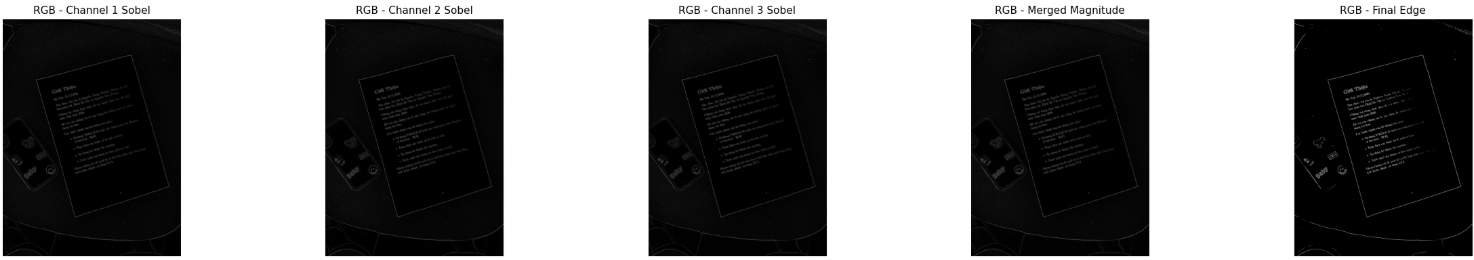
\includegraphics[width=\textwidth]{sobel_rgb_t60.png}
\caption{Quá trình phát hiện biên  Sobel + Thresholding trên hệ màu RGB với ngưỡng $T=60$}
\end{figure}

\begin{figure}[H]
\centering
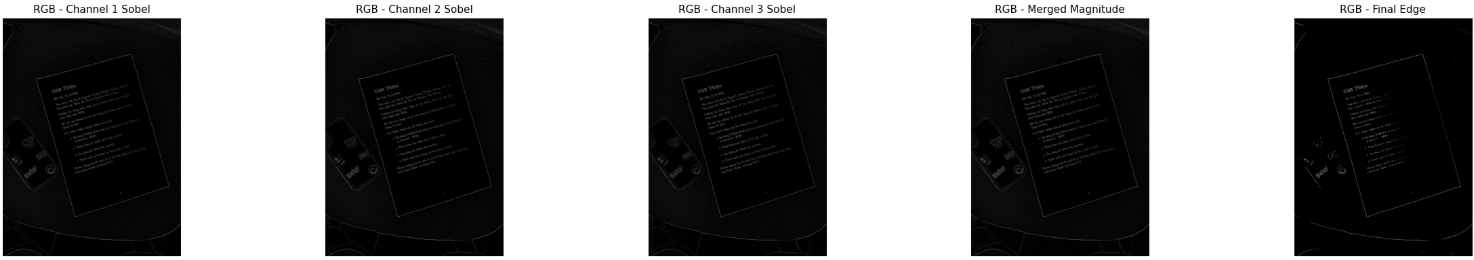
\includegraphics[width=\textwidth]{sobel_rgb_t90.png}
\caption{Quá trình phát hiện biên  Sobel + Thresholding trên hệ màu RGB với ngưỡng $T=90$}
\end{figure}

\textbf{Nhận xét:}

Cả ba kênh R, G, B đều phát hiện biên khá đồng đều, cho thấy thông tin biên chủ yếu đến từ sự thay đổi cường độ sáng chứ không phụ thuộc nhiều vào màu sắc riêng lẻ.

Khi gộp các kênh, biên của tài liệu trở nên rõ và liên tục hơn. Tuy nhiên, các chi tiết nền như vân bàn, mép ghế hay vật dụng xung quanh cũng bị giữ lại, tạo ra nhiều contour rác trong ảnh Final Edge.

\subsubsection{Hệ màu RGB được cân bằng sáng trên HSV}

Để giải quyết vấn đề ảnh thiếu sáng hoặc ánh sáng phân bố không đều (bóng đổ), hệ thống thực hiện một bước tiền xử lý: chuyển ảnh RGB sang hệ HSV, áp dụng cân bằng biểu đồ tần suất thích ứng (CLAHE) lên riêng kênh V (Độ sáng), sau đó chuyển ngược lại về hệ RGB để thực hiện dò biên đa kênh.

\begin{figure}[H]
\centering
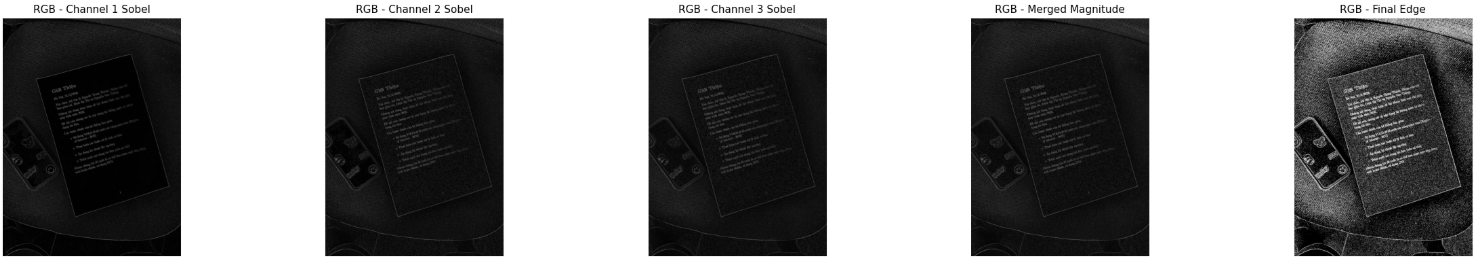
\includegraphics[width=\textwidth]{sobel_rgb_hsv_t30.png}
\caption{Phát hiện biên Sobel trên RGB (đã cân bằng sáng qua HSV) với $T=30$}
\end{figure}

\begin{figure}[H]
\centering
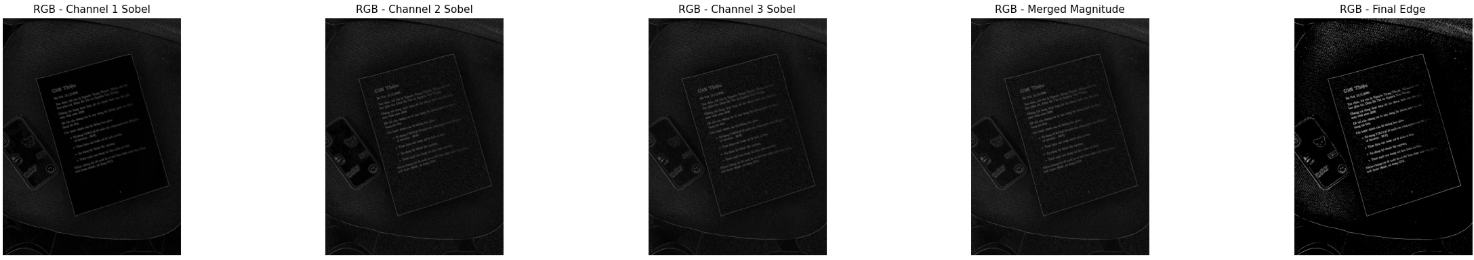
\includegraphics[width=\textwidth]{sobel_rgb_hsv_t60.png}
\caption{Phát hiện biên Sobel trên RGB (đã cân bằng sáng qua HSV) với $T=60$}
\end{figure}

\begin{figure}[H]
\centering
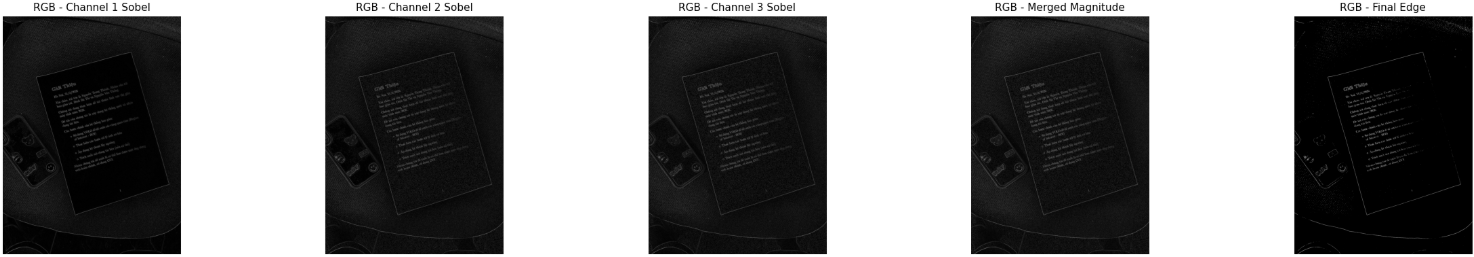
\includegraphics[width=\textwidth]{sobel_rgb_hsv_t90.png}
\caption{Phát hiện biên Sobel trên RGB (đã cân bằng sáng qua HSV) với $T=90$}
\end{figure}

\textbf{Nhận xét:}

Cân bằng sáng qua kênh V trong hệ HSV giúp tăng tương phản rất mạnh, làm viền tờ giấy và chữ viết nổi bật hơn so với ảnh RGB gốc, đồng thời hỗ trợ Sobel phát hiện các đoạn biên bị chìm trong vùng tối. Tuy nhiên, việc tăng sáng quá mạnh cũng làm nhiễu nền như vân gỗ, mép vật thể, texture và vùng phản xạ sáng bị khuếch đại theo. Vì vậy, ở ngưỡng thấp T=30, ảnh biên xuất hiện nhiều nhiễu rác; ngay cả khi tăng lên T=90, nền vẫn còn nhiều biên thừa, gây khó khăn cho các bước tách nền và tìm contour sau này.

\subsubsection{Hệ màu RGB được cân bằng sáng trên LAB}

Tiếp tục hướng tiếp cận tiền xử lý, hệ thống thử nghiệm cân bằng sáng (CLAHE) trên kênh L của không gian LAB thay vì kênh V của HSV. Sau khi cân bằng, ảnh được chuyển ngược về RGB để áp dụng toán tử Sobel.

\begin{figure}[H]
\centering
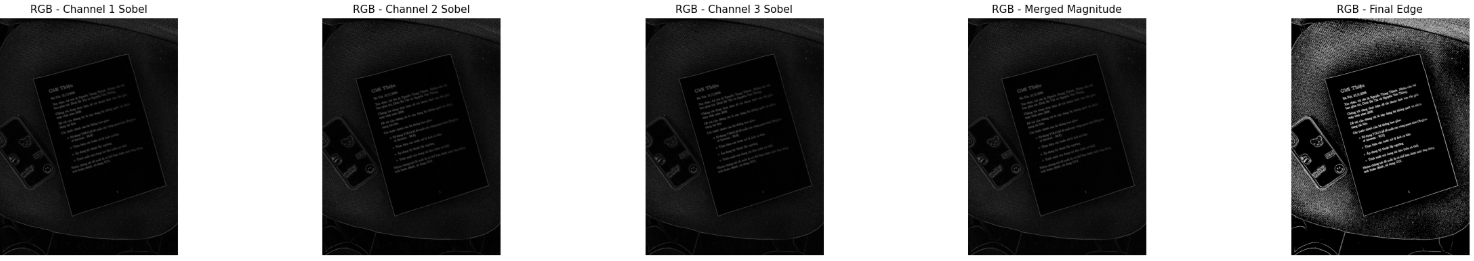
\includegraphics[width=\textwidth]{sobel_rgb_lab_t30.png}
\caption{Phát hiện biên Sobel trên RGB (đã cân bằng sáng qua LAB) với $T=30$}
\end{figure}

\begin{figure}[H]
\centering
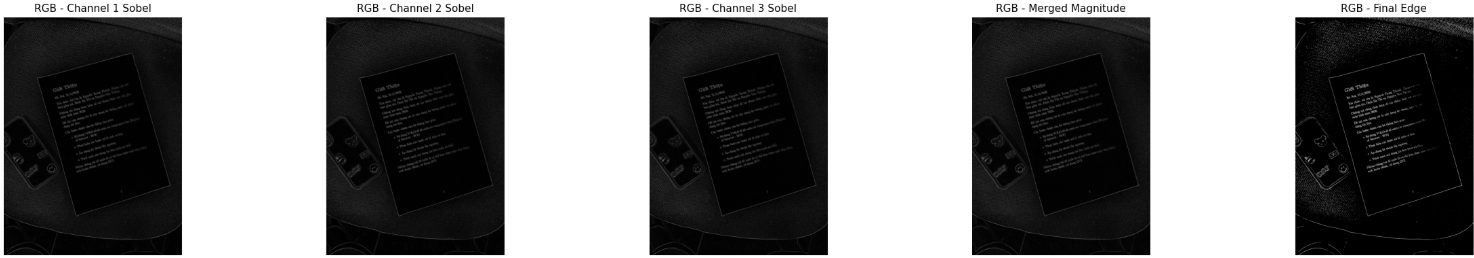
\includegraphics[width=\textwidth]{sobel_rgb_lab_t60.png}
\caption{Phát hiện biên Sobel trên RGB (đã cân bằng sáng qua LAB) với $T=60$}
\end{figure}

\begin{figure}[H]
\centering
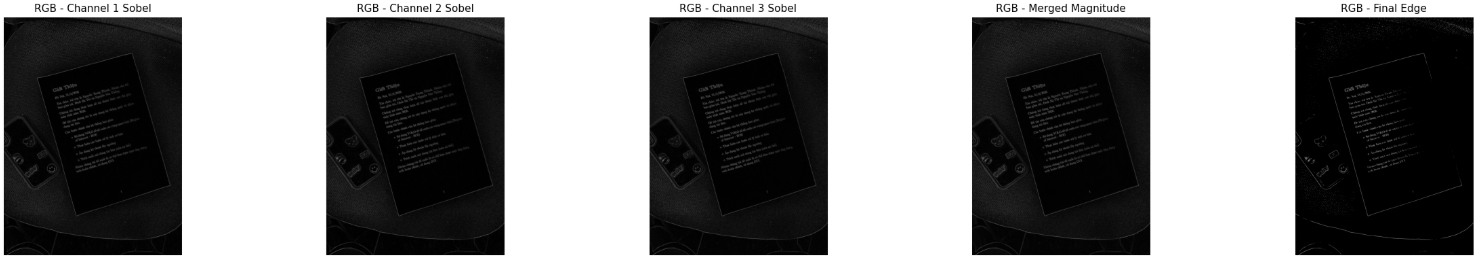
\includegraphics[width=\textwidth]{sobel_rgb_lab_t90.png}
\caption{Phát hiện biên Sobel trên RGB (đã cân bằng sáng qua LAB) với $T=90$}
\end{figure}

\textbf{Nhận xét:}

Cân bằng sáng trên hệ LAB giúp tăng độ tương phản giữa tài liệu và nền một cách ổn định, làm khung viền và nét chữ rõ hơn mà không bị đẩy sáng quá mức. So với HSV, kết quả biên từ LAB sạch hơn, giảm đáng kể nhiễu do phản xạ sáng, bóng đổ và texture nền. Nhờ tách riêng kênh sáng L khỏi hai kênh màu A, B, phương pháp này giúp CLAHE tăng tương phản hiệu quả mà ít khuếch đại nhiễu màu, nên phù hợp hơn cho bài toán phát hiện biên tài liệu.

\subsection{Thuật toán Canny}

Khác với Sobel chỉ sử dụng một mức phân ngưỡng cứng, thuật toán Canny sử dụng cơ chế ngưỡng kép (Hysteresis Thresholding) \cite{canny1986} gồm ngưỡng thấp và ngưỡng cao để theo vết và nối liền các đường biên. 

\subsubsection{Trên ảnh xám}

Thực nghiệm đầu tiên của thuật toán Canny được tiến hành trên ảnh xám (đã qua bước tiền xử lý làm mờ Gaussian Blur để giảm nhiễu hạt) với hai bộ ngưỡng khảo sát là $(50, 150)$ và $(100, 200)$.

\begin{figure}[H]
\centering
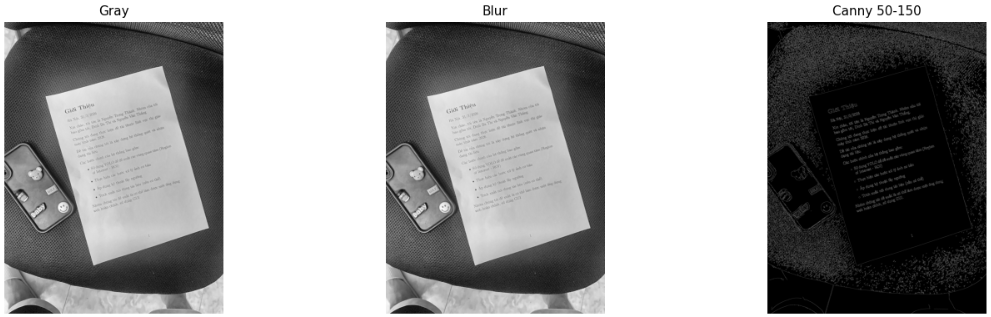
\includegraphics[width=\textwidth]{canny_gray_50_150.png}
\caption{Phát hiện biên Canny trên ảnh xám với bộ ngưỡng (50, 150)}
\end{figure}

\begin{figure}[H]
\centering
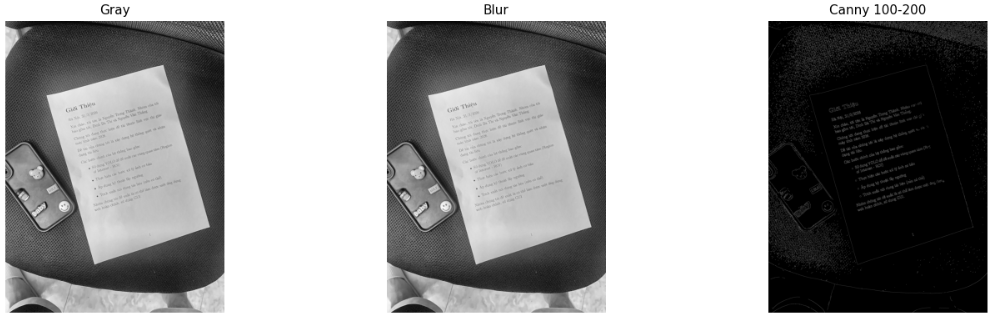
\includegraphics[width=\textwidth]{canny_gray_100_200.png}
\caption{Phát hiện biên Canny trên ảnh xám với bộ ngưỡng (100, 200)}
\end{figure}

\textbf{Nhận xét:}

Với bộ ngưỡng (50, 150), Canny bắt biên rất nhạy nên giữ lại nhiều chi tiết như mép giấy, chữ viết và cả họa tiết nền, nhưng đồng thời tạo ra nhiều nhiễu rác, gây khó khăn cho bước tìm contour. Ngược lại, bộ ngưỡng (100, 200) cho ảnh biên sạch hơn, loại bỏ tốt các biên yếu và nhiễu nền, giúp khung viền tờ giấy nổi bật hơn, dù có thể làm đứt nhẹ một số nét mờ. Vì mục tiêu chính của bài toán scan tài liệu là xác định khung viền ngoài, nên chọn ngưỡng (100, 200) là hợp lý hơn.


% \subsubsection{Hệ màu HSV}

% Để đối chiếu với ảnh xám, thuật toán Canny tiếp tục được thử nghiệm trên không gian màu HSV. Quá trình dò biên được thực hiện độc lập trên 3 kênh H (Màu sắc), S (Độ bão hòa), V (Độ sáng), sau đó tổng hợp lại thành một ảnh biên duy nhất (Merged edge) thông qua phép toán logic OR. 

% \begin{figure}[H]
% \centering
% 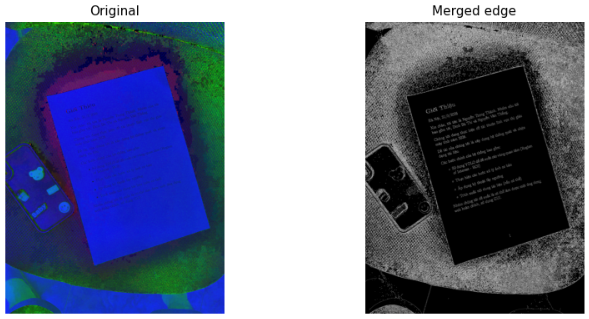
\includegraphics[width=0.8\textwidth]{canny_hsv_50_150.png}
% \caption{Phát hiện biên Canny gộp kênh trên hệ HSV với bộ ngưỡng (50, 150)}
% \end{figure}

% \begin{figure}[H]
% \centering
% 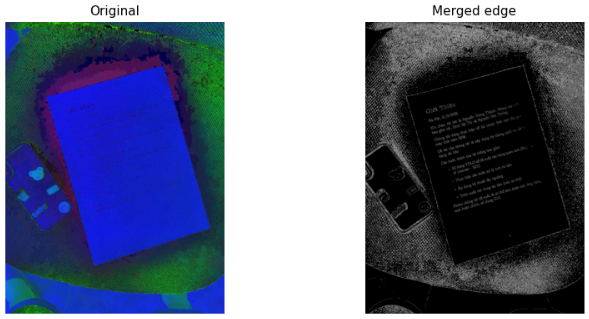
\includegraphics[width=0.8\textwidth]{canny_hsv_100_200.png}
% \caption{Phát hiện biên Canny gộp kênh trên hệ HSV với bộ ngưỡng (100, 200)}
% \end{figure}

% \textbf{Nhận xét thực nghiệm:}

% \begin{itemize}
%     \item \textbf{Hiện tượng khuếch đại nhiễu:} Trái ngược hoàn toàn với sự "sạch sẽ" của ảnh xám, ảnh biên tổng hợp từ hệ HSV ngập tràn trong lượng nhiễu khổng lồ. Toàn bộ cấu trúc lưới của mặt ghế bị bắt lại cực kỳ chi tiết, tạo thành một mạng lưới rác trắng xóa bao trùm cả bức ảnh.
%     \item \textbf{Nguyên nhân:} Các kênh H và S vô cùng nhạy cảm với những biến thiên vi mô về màu sắc và ánh sáng của môi trường. Điểm mạnh của Canny là cơ chế nối biên (Hysteresis Thresholding), nhưng trong trường hợp này, nó lại phản tác dụng khi vô tình "hàn gắn" các chấm nhiễu li ti từ kênh H và S thành những mảng contour rác liên tục.
%     \item \textbf{Đánh giá tác động của ngưỡng:} Khác với ảnh xám, việc tăng ngưỡng lên $(100, 200)$ trên HSV gần như không mang lại sự cải thiện đáng kể nào. Lượng nhiễu từ nền vẫn quá áp đảo, khiến khung viền thực sự của tờ giấy bị chìm lấp hoàn toàn.
% \end{itemize}

% \textbf{Kết luận:} Việc áp dụng Canny đa kênh trên hệ HSV và gộp kết quả là phương pháp \textbf{không khả thi} đối với bài toán scan tài liệu trên nền phức tạp. Sự dư thừa thông tin từ kênh màu sắc đã phá vỡ hoàn toàn khả năng nhận diện hình học (tứ giác) của thuật toán ở các bước sau.

% \subsubsection{Hệ màu LAB}

% Hệ không gian màu CIELAB tiếp tục được đưa vào thử nghiệm với thuật toán Canny. Tương tự quy trình trước, ảnh biên tổng hợp (Merged edge) được tạo ra từ việc gộp các đường biên dò được độc lập trên cả 3 kênh L, A và B.

% \begin{figure}[H]
% \centering
% 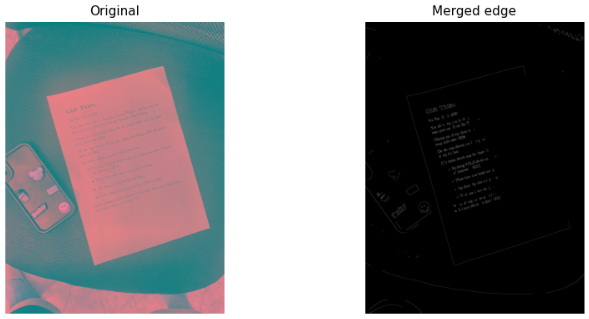
\includegraphics[width=0.8\textwidth]{canny_lab_50_150.png} % Nhớ đổi tên file ảnh tương ứng
% \caption{Phát hiện biên Canny gộp kênh trên hệ LAB với bộ ngưỡng (50, 150)}
% \end{figure}

% \begin{figure}[H]
% \centering
% 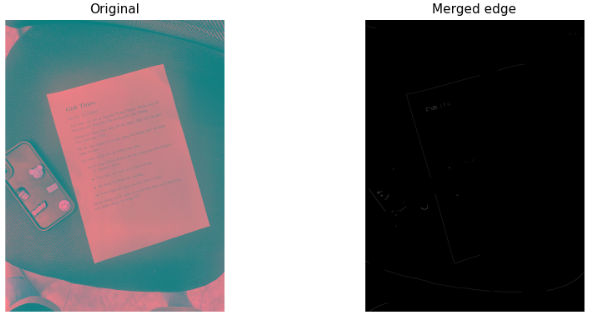
\includegraphics[width=0.8\textwidth]{canny_lab_100_200.png} % Nhớ đổi tên file ảnh tương ứng
% \caption{Phát hiện biên Canny gộp kênh trên hệ LAB với bộ ngưỡng (100, 200)}
% \end{figure}

% \textbf{Nhận xét thực nghiệm:}

% \begin{itemize}
%     \item \textbf{Khả năng kháng nhiễu ấn tượng:} Khác biệt hoàn toàn với "thảm họa" nhiễu của hệ HSV, ảnh biên gộp từ hệ LAB vô cùng sạch sẽ. Cấu trúc lưới phức tạp của mặt ghế (texture) gần như bị triệt tiêu hoàn toàn. Điều này minh chứng cho sức mạnh của LAB: kênh L đảm nhiệm việc vạch ranh giới sáng/tối rất tốt, trong khi kênh màu (A, B) ổn định và không sinh ra các contour rác do bóng đổ.
%     \item \textbf{Đánh giá tác động của bộ ngưỡng:}
%     \begin{itemize}
%         \item \textbf{Ngưỡng (50, 150):} Kết quả đạt mức cân bằng xuất sắc. Khung viền biên của tờ giấy liền mạch, rõ nét, các dòng chữ bên trong được giữ lại khá đầy đủ trong khi nhiễu nền ở mức tối thiểu.
%         \item \textbf{Ngưỡng (100, 200):} Ảnh nền trở nên đen tuyệt đối (sạch hoàn toàn). Tuy nhiên, cặp ngưỡng này lại quá "mạnh tay" khi xóa sổ gần hết các nét chữ bên trong tài liệu, đồng thời làm viền của tờ giấy trở nên mỏng manh hơn và có nguy cơ đứt gãy cục bộ.
%     \end{itemize}
% \end{itemize}

% \textbf{Kết luận:} Việc áp dụng thuật toán Canny đa kênh trên hệ LAB mang lại hiệu quả rất cao. Nhờ khả năng cô lập độ sáng và màu sắc ưu việt, hệ LAB cho phép sử dụng cặp ngưỡng thấp \textbf{(50, 150)} để bảo toàn toàn vẹn khung tài liệu mà không phải lo lắng về việc bùng nổ nhiễu rác từ môi trường như hệ HSV.

\subsubsection{Hệ màu RGB}

Thuật toán Canny được triển khai độc lập trên 3 kênh R, G, B. Do đặc tính của ảnh màu, mỗi kênh sẽ nhạy cảm và phát hiện ra những đoạn biên khác nhau. Sau đó, kết quả từ 3 kênh được tổng hợp lại thành ảnh Merged Edge thông qua phép toán logic OR.

\begin{figure}[H]
\centering
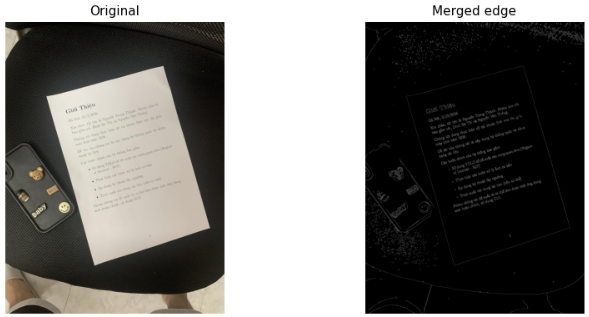
\includegraphics[width=0.8\textwidth]{canny_rgb_50_150.png} % Đổi tên file tương ứng
\caption{Phát hiện biên Canny gộp kênh trên hệ RGB với bộ ngưỡng (50, 150)}
\end{figure}

\begin{figure}[H]
\centering
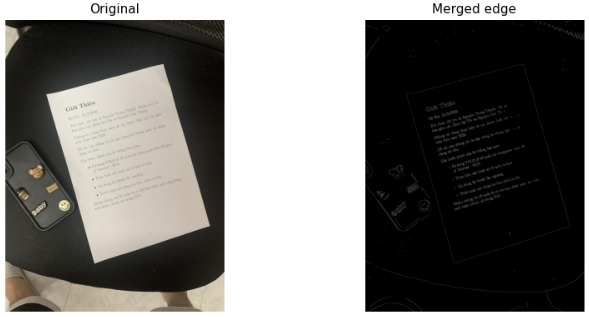
\includegraphics[width=0.8\textwidth]{canny_rgb_100_200.png} % Đổi tên file tương ứng
\caption{Phát hiện biên Canny gộp kênh trên hệ RGB với bộ ngưỡng (100, 200)}
\end{figure}

\textbf{Nhận xét:}

Với ảnh RGB gốc, ba kênh màu thường chứa rất nhiều thông tin bề mặt (texture) của nền. Khi gộp bằng phép OR, toàn bộ các dải biên này (kể cả biên rác từ vân bàn, nền vải, bóng đổ) đều được giữ lại cộng dồn. Hậu quả là bức ảnh Merged Edge, dù ở bộ ngưỡng $(100, 200)$, vẫn xuất hiện tình trạng nhiễu lưới khá rõ rệt xung quanh tài liệu.


\subsubsection{Hệ màu RGB được cân bằng sáng qua HSV}

Nhằm mục đích làm rõ biên tài liệu, nhóm thử nghiệm áp dụng cân bằng sáng CLAHE trên kênh V của hệ HSV trước khi chuyển về RGB để chạy Canny.

\begin{figure}[H]
\centering
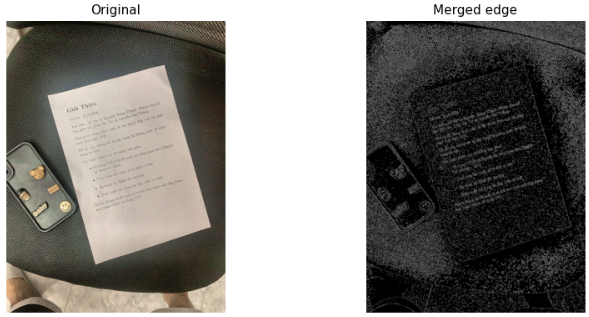
\includegraphics[width=0.8\textwidth]{canny_rgb_hsv_50_150.png} % Đổi tên file tương ứng
\caption{Phát hiện biên Canny trên RGB (đã cân bằng sáng qua HSV) với (50, 150)}
\end{figure}

\begin{figure}[H]
\centering
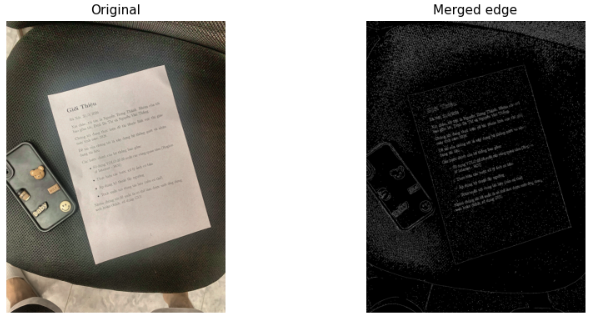
\includegraphics[width=0.8\textwidth]{canny_rgb_hsv_100_200.png} % Đổi tên file tương ứng
\caption{Phát hiện biên Canny trên RGB (đã cân bằng sáng qua HSV) với (100, 200)}
\end{figure}

\textbf{Nhận xét:}

Việc cân bằng sáng thực sự đã đẩy độ tương phản lên rất cao, nhưng đối với thuật toán Canny, đây lại là một điểm trừ lớn. Cơ chế dò biên theo biến thiên gradient của Canny bị đánh lừa bởi sự gia tăng tương phản này. Kết quả là không chỉ biên giấy rõ hơn, mà toàn bộ các texture nền (như mặt lưới của ghế) cũng bị khuếch đại mạnh mẽ, khiến ảnh bị nhiễu hạt (noise) trầm trọng, làm sai lệch hoàn toàn quá trình xấp xỉ đa giác.


\subsubsection{Hệ màu RGB được cân bằng sáng qua LAB}

Tương tự như trên, thực nghiệm cuối cùng áp dụng CLAHE trên kênh L của hệ LAB để cân bằng sáng trước khi chạy Canny đa kênh RGB.

\begin{figure}[H]
\centering
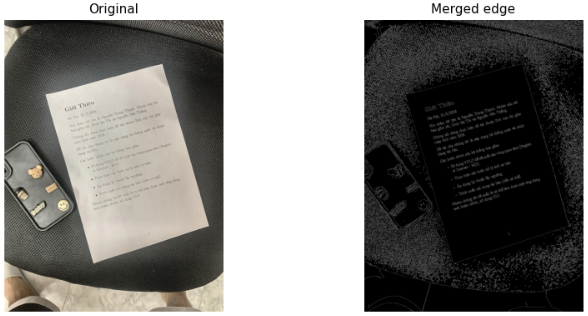
\includegraphics[width=0.8\textwidth]{canny_rgb_lab_50_150.png} % Đổi tên file tương ứng
\caption{Phát hiện biên Canny trên RGB (đã cân bằng sáng qua LAB) với (50, 150)}
\end{figure}

\begin{figure}[H]
\centering
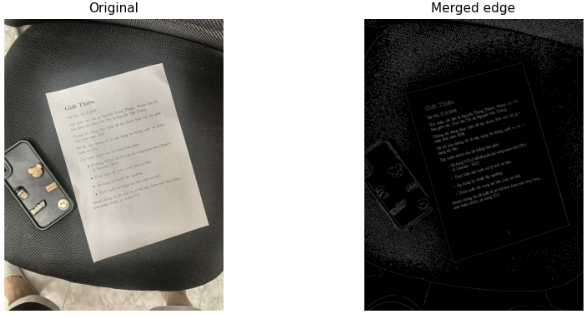
\includegraphics[width=0.8\textwidth]{canny_rgb_lab_100_200.png} % Đổi tên file tương ứng
\caption{Phát hiện biên Canny trên RGB (đã cân bằng sáng qua LAB) với (100, 200)}
\end{figure}

\textbf{Nhận xét chung:}

Qua thực nghiệm, Canny khi áp dụng trên nhiều kênh màu như RGB, HSV hoặc LAB có thể phát hiện thêm nhiều chi tiết biên, nhưng dễ làm cộng dồn nhiễu từ từng kênh. Vì vậy, kết quả sau khi gộp biên thường xuất hiện nhiều nét nhỏ, đứt gãy và nhiễu nền. Cách ổn định hơn là chạy Canny trên ảnh xám hoặc kênh L của hệ LAB, kết hợp với ngưỡng cao $(100, 200)$ để loại bỏ nhiễu tốt hơn.

Đối với Sobel kết hợp với Threshold, ảnh xám cho kết quả khá tốt trong việc làm nổi bật biên tờ giấy và chữ do giảm ảnh hưởng của màu sắc. Tuy nhiên, phương pháp này vẫn nhạy với nền phức tạp và ánh sáng không đều. Khi áp dụng trên ảnh đã cân bằng sáng bằng LAB, biên tài liệu và nét chữ rõ hơn, đặc biệt trong các vùng tối hoặc bị bóng đổ, nhưng vẫn cần chọn ngưỡng phù hợp để tránh giữ lại nhiễu nền.

\section{Phát hiện Contour và hiệu chỉnh phối cảnh}

Sau quá trình phát hiện biên, việc tìm kiếm và bao đóng contour của tài liệu là bước quyết định để thực hiện phép biến đổi phối cảnh. Dựa trên thực nghiệm, nhóm đã phân tích cấu hình dò tìm thông qua việc điều chỉnh các phép biến đổi hình thái học, kích thước kernel và không gian màu đầu vào.

\subsection{Một số kết quả đạt được}

Việc thực nghiệm tìm biên trên ảnh RGB đã được cân bằng sáng và ảnh Gray đã được cân bằng sáng cho
kết quả nổi bật hơn các trường hợp còn lại. Biên được phát hiện dày và liên tục, vì vậy phương pháp tìm Contour sẽ được thực nghiệm sau khi đã áp dụng hai phương pháp trên.

Một số kết quả nổi bật đã đạt được:

\begin{figure}[H]
    \centering

    \begin{subfigure}{0.9\textwidth}
        \centering
        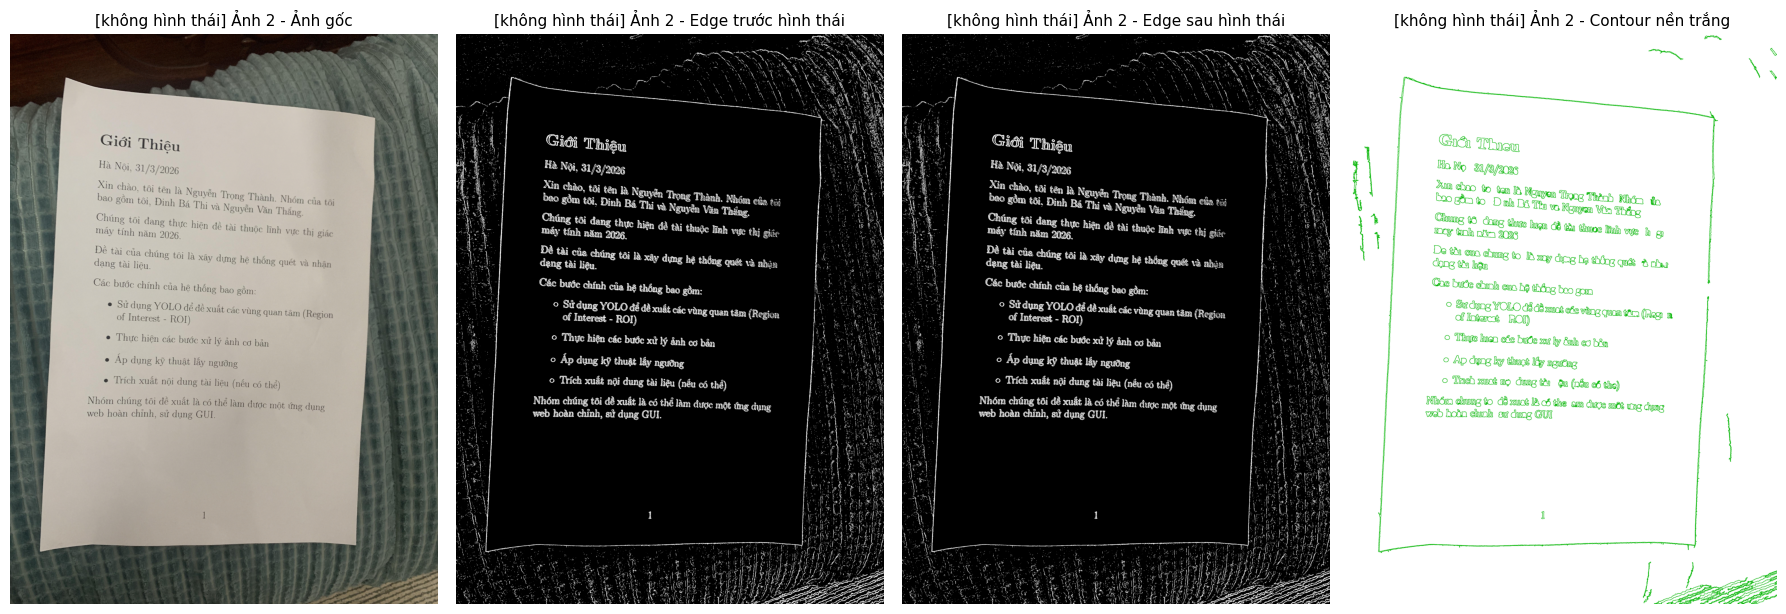
\includegraphics[width=\textwidth]{contour_1.png}
        \caption{Ảnh 1 - Gray}
    \end{subfigure}

    \vspace{0.1cm}

    \begin{subfigure}{0.9\textwidth}
        \centering
        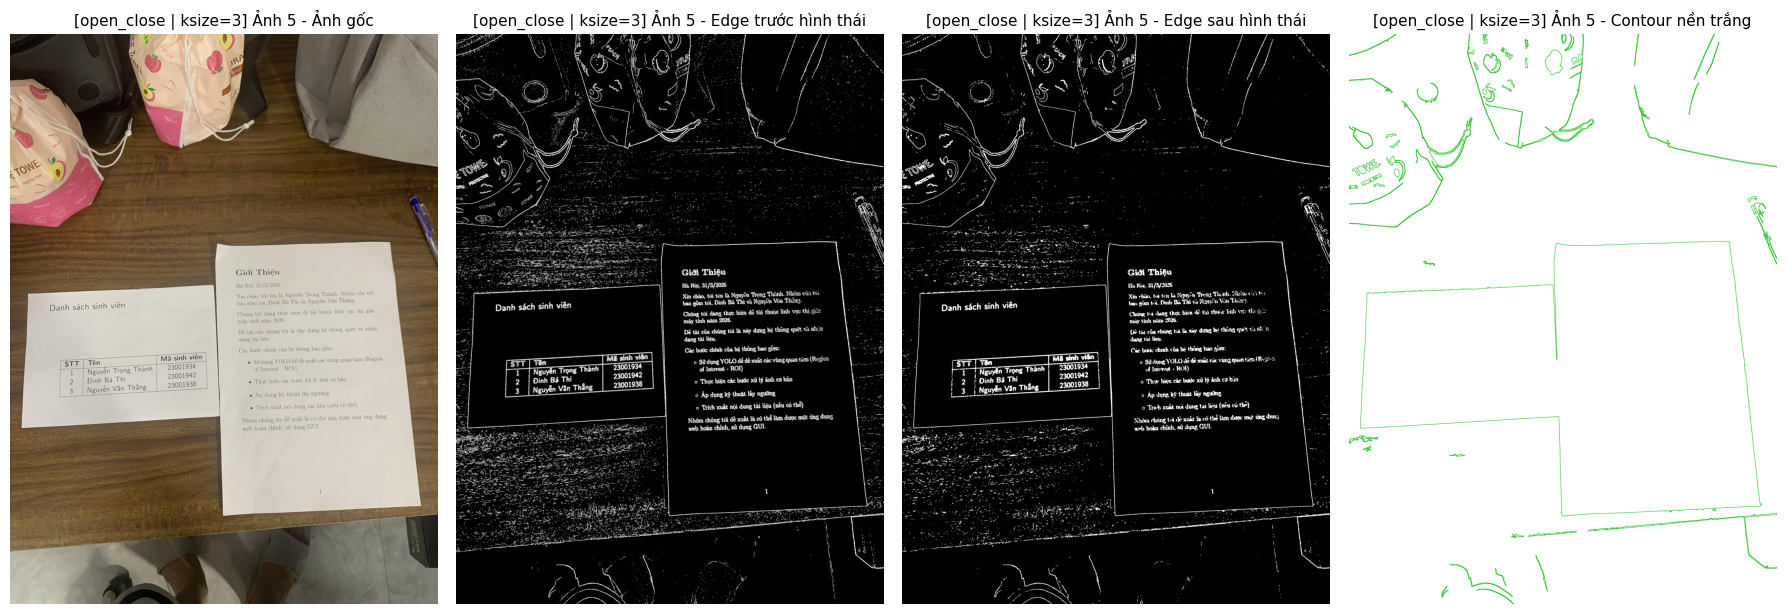
\includegraphics[width=\textwidth]{contour_3.png}
        \caption{Ảnh 2 - Gray}
    \end{subfigure}

    \vspace{0.1cm}

    \begin{subfigure}{0.9\textwidth}
        \centering
        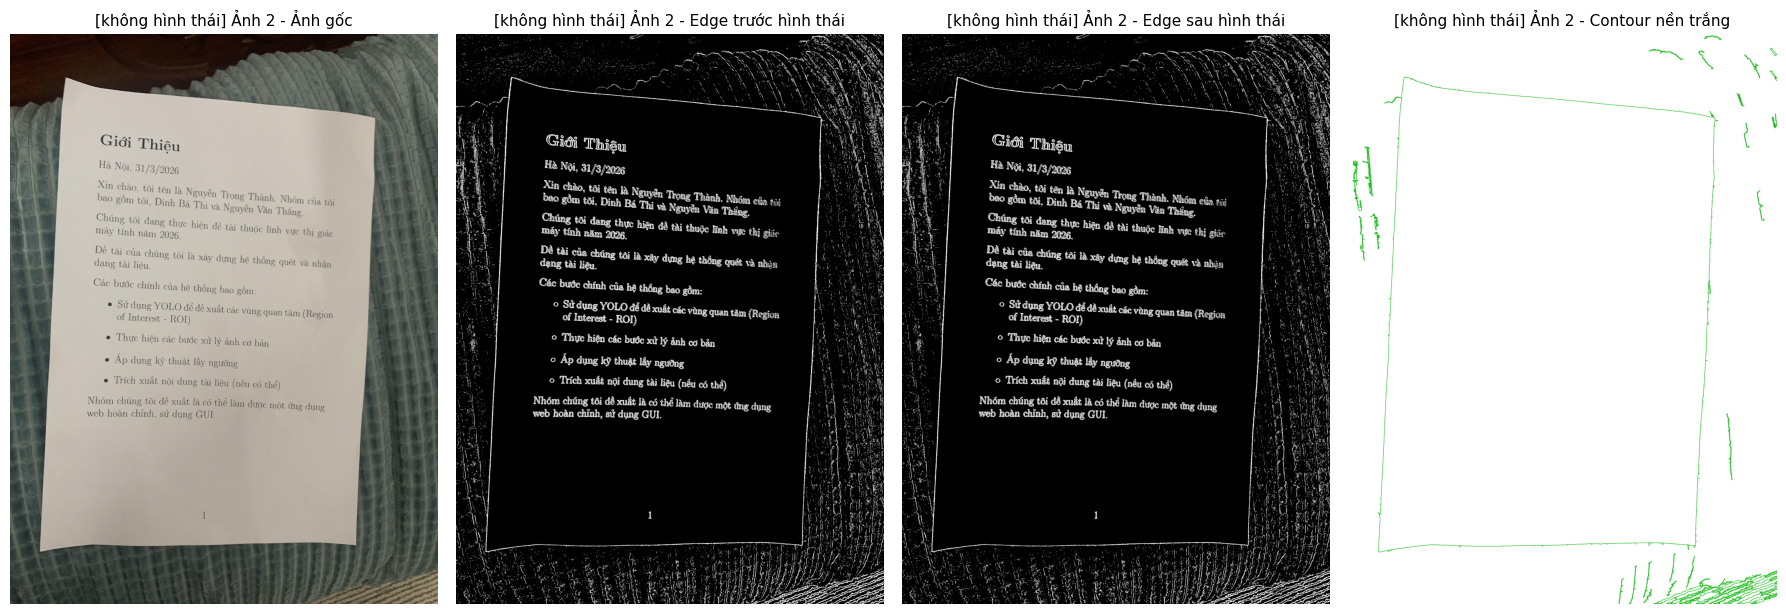
\includegraphics[width=\textwidth]{contour_2.png}
        \caption{Ảnh 3 - RGB cân bằng sáng}
    \end{subfigure}

    \vspace{0.1cm}

    \begin{subfigure}{0.9\textwidth}
        \centering
        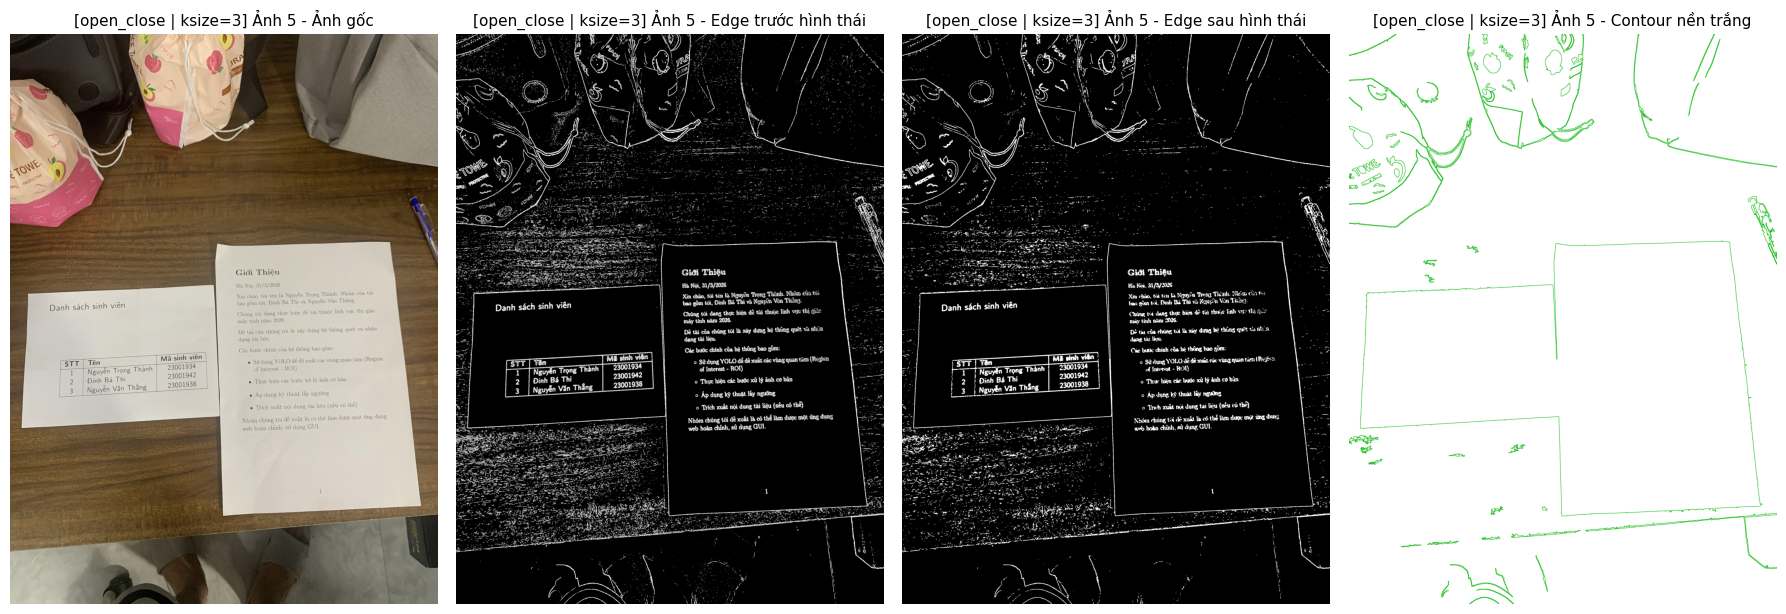
\includegraphics[width=\textwidth]{contour_4.png}
        \caption{Ảnh 4 - RGB cân bằng sáng}
    \end{subfigure}

    \caption{Một số kết quả phát hiện Contour.}
    \label{fig:gray_vs_rgb_equalized}
\end{figure}


\subsection{Đánh giá ảnh hưởng của Biến đổi hình thái học}

Để làm sạch nhiễu và nối liền các đoạn biên bị đứt gãy, hệ thống khảo sát các phép toán hình thái học (Morphological Operations) trước khi tiến hành dò contour. Dưới đây là thực nghiệm trên ảnh CLAHE GRAY với một mẫu ảnh có nền phức tạp (ga giường kẻ sọc).

% --- PHẦN 1 CỦA HÌNH (Gồm Không hình thái và k=3) ---
\begin{figure}[H]
    \centering
    % Hàng 1: Không hình thái
    \begin{subfigure}[b]{\textwidth}
        \centering
        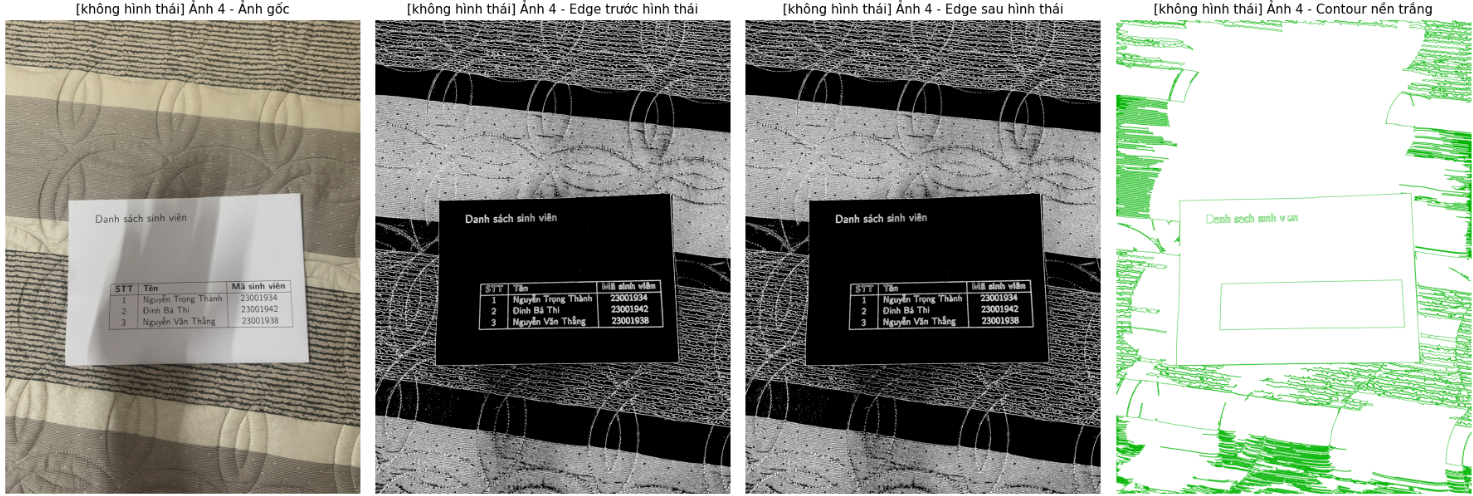
\includegraphics[width=\textwidth]{anh4_khong_hinh_thai.png}
        \caption{Không sử dụng: Contour bị nhiễu nặng bởi các đường sọc của nền.}
    \end{subfigure}
    
    \vspace{0.5cm} % Khoảng cách giữa các ảnh
    
    % Hàng 2: Open - Close k=3
    \begin{subfigure}[b]{\textwidth}
        \centering
        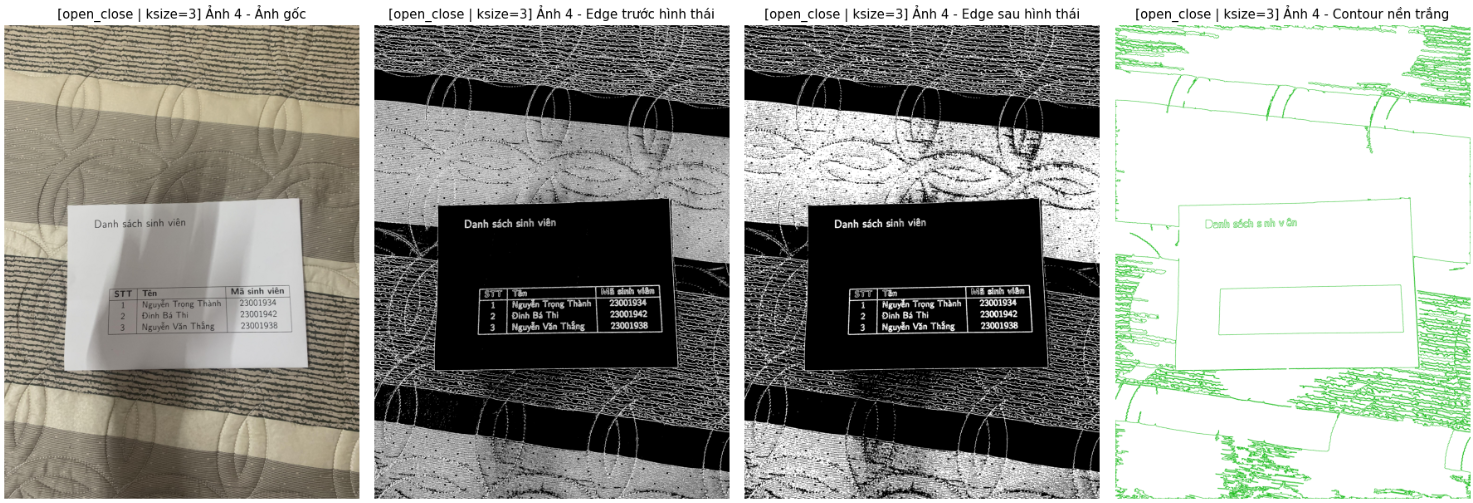
\includegraphics[width=\textwidth]{anh4_open_close_k3.png}
        \caption{Open rồi Close (k=3): Tác động quá nhẹ, chưa thể xóa được nhiễu nền sọc và viền tài liệu vẫn bị đứt gãy.}
    \end{subfigure}

    \vspace{0.5cm}

    % Hàng 3: Close - Open k=3
    \begin{subfigure}[b]{\textwidth}
        \centering
        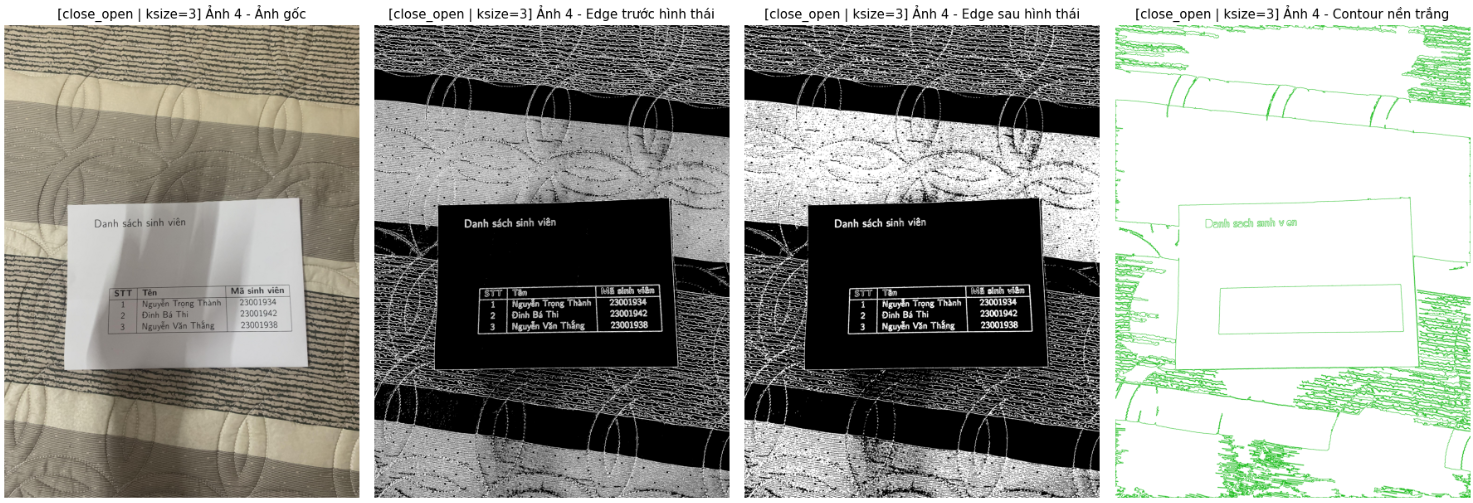
\includegraphics[width=\textwidth]{anh4_close_open_k3.png}
        \caption{Close rồi Open (k=3): Khả năng nối viền có cải thiện nhưng tác động vẫn chưa đủ mạnh, rác nền sọc vẫn còn rất nhiều.}
    \end{subfigure}
    
    \caption{So sánh tác động của thứ tự biến đổi hình thái học lên chất lượng trích xuất contour}
    \label{fig:morphology_compare_1}
\end{figure}

% --- PHẦN 2 CỦA HÌNH (Gồm k=5) - Sẽ tự động nhảy sang trang tiếp theo ---
\begin{figure}[H]
    \centering
    % Hàng 4: Open - Close k=5
    \begin{subfigure}[b]{\textwidth}
        \centering
        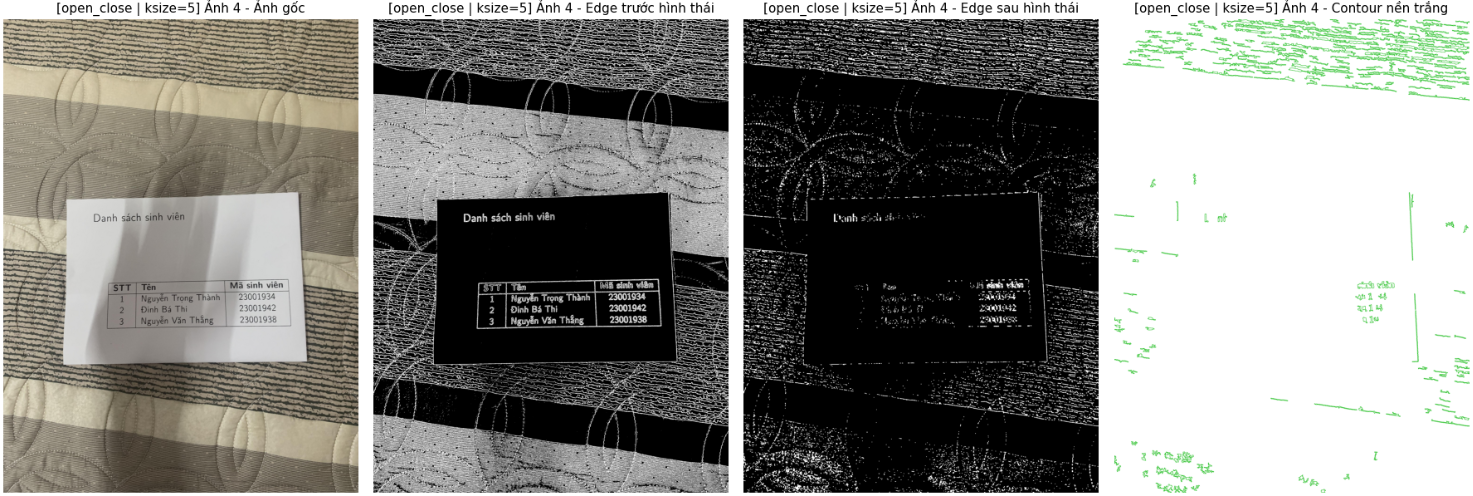
\includegraphics[width=\textwidth]{anh4_open_close_k5.png}
        \caption{Open rồi Close (k=5): Xóa được rác nhưng làm đứt gãy hoàn toàn viền tài liệu.}
    \end{subfigure}
    
    \vspace{0.5cm}
    
    % Hàng 5: Close - Open k=5
    \begin{subfigure}[b]{\textwidth}
        \centering
        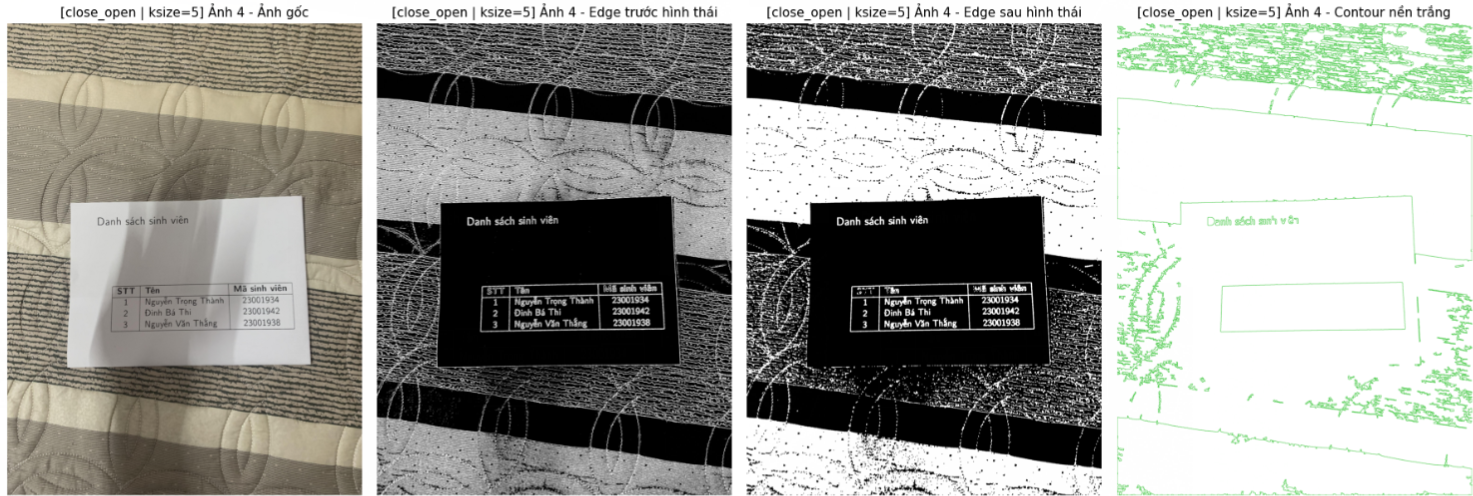
\includegraphics[width=\textwidth]{anh4_close_open_k5.png}
        \caption{Close rồi Open (k=5): Viền tài liệu được khép kín liền mạch, tạo thành khung chữ nhật hoàn chỉnh.}
    \end{subfigure}
    
    \caption{So sánh tác động của thứ tự biến đổi hình thái học lên chất lượng trích xuất contour (Tiếp theo)}
    \label{fig:morphology_compare_2}
\end{figure}

\textbf{Nhận xét:}
\begin{itemize}
    \item \textbf{Không sử dụng:} Contour bao quanh tài liệu bị đứt đoạn, rời rạc và lẫn nhiều viền rác.
    \item \textbf{Open rồi Close:} Xóa được nhiễu nhưng vô tình làm đứt gãy viền tài liệu (do các chi tiết biên nhỏ bị ăn mòn trước khi kịp nối lại).
    \item \textbf{Close rồi Open (Tối ưu):} Phép Close lập tức nối liền các đoạn biên bị hở, sau đó phép Open dọn dẹp nhiễu rác thừa. Quá trình này tạo ra khung tài liệu khép kín và liền mạch, mang lại điều kiện lý tưởng nhất cho thuật toán xấp xỉ đa giác ở bước sau.
\end{itemize}

\subsection{Đánh giá ảnh hưởng của kích thước Kernel}

Cố định phương pháp \textbf{Close rồi Open}, nhóm tiếp tục khảo sát mức độ tác động của kích thước bộ lọc (Kernel size $k$). Dưới đây là kết quả thực nghiệm trên ảnh có nền cấu trúc lưới (Ghế đen).

\begin{figure}[H]
    \centering
    % Hàng 1: Kernel = 3
    \begin{subfigure}[b]{\textwidth}
        \centering
        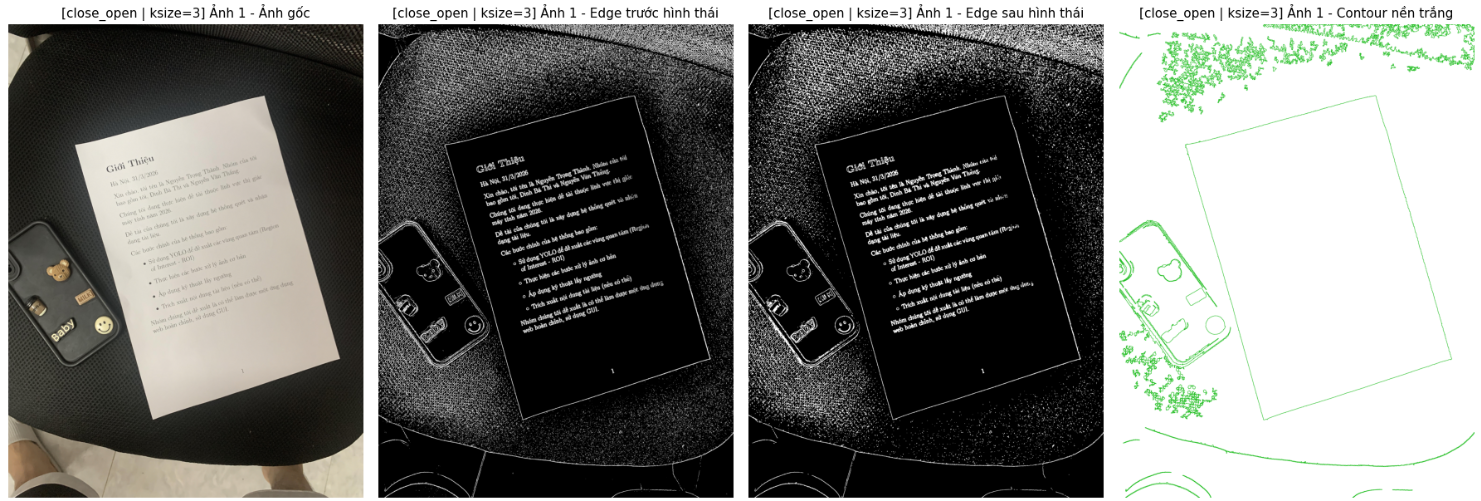
\includegraphics[width=0.8\textwidth]{kernel_3.png}
        \caption{Kernel $k=3$: Viền tài liệu được bảo toàn khá đầy đủ nhưng khả năng khử nhiễu từ nền lưới chưa mạnh, vẫn còn nhiều dải contour rác.}
    \end{subfigure}
    
    \vspace{0.5cm} % Khoảng cách giữa các ảnh
    
    % Hàng 2: Kernel = 5
    \begin{subfigure}[b]{\textwidth}
        \centering
        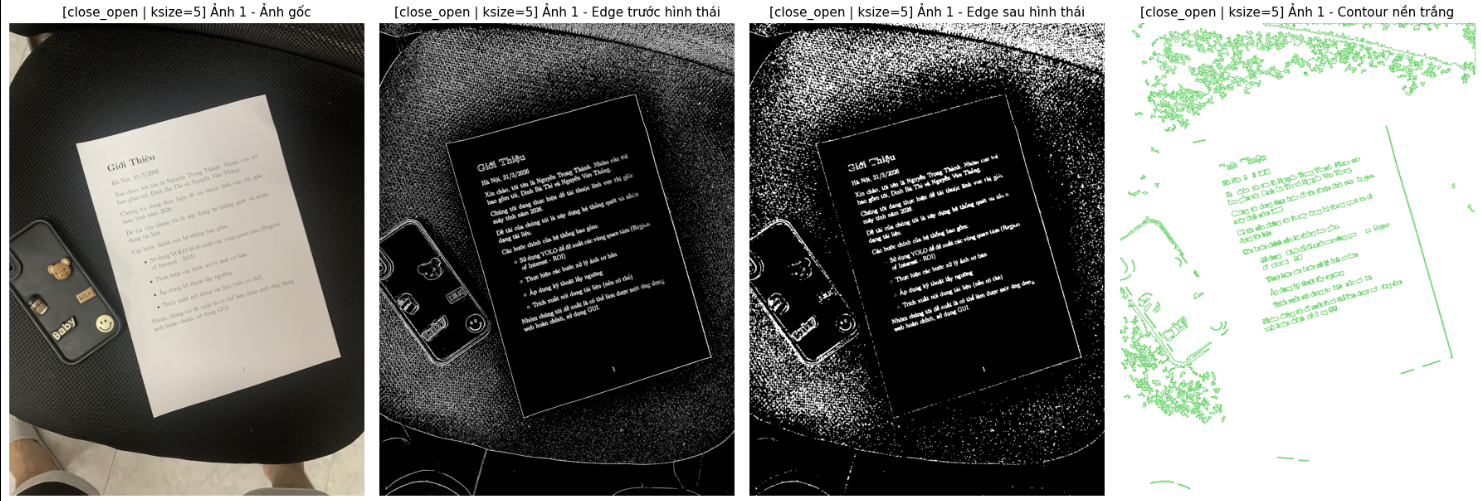
\includegraphics[width=0.8\textwidth]{kernel_5.png}
        \caption{Kernel $k=5$: Nhiễu nền giảm đáng kể, viền giấy tuy có bị tác động nhẹ nhưng vẫn giữ được hình dáng tổng thể để xấp xỉ khung chữ nhật.}
    \end{subfigure}
    
    \vspace{0.5cm}
    
    % Hàng 3: Kernel = 7
    \begin{subfigure}[b]{\textwidth}
        \centering
        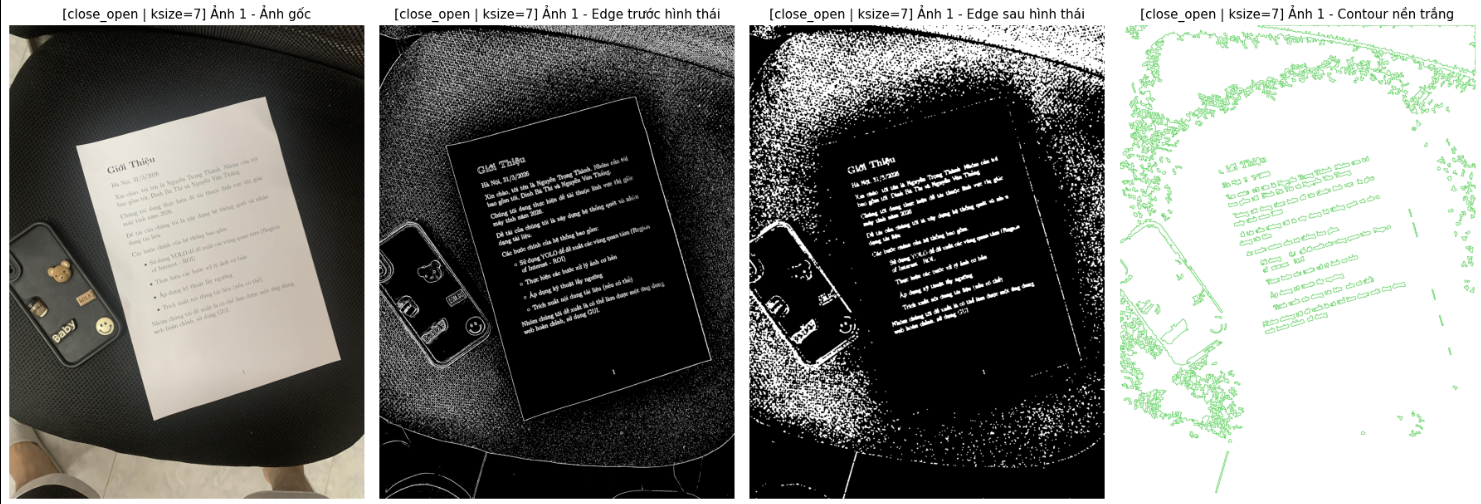
\includegraphics[width=0.8\textwidth]{kernel_7.png}
        \caption{Kernel $k=7$: Tác động quá mạnh làm đứt gãy nghiêm trọng, cạnh phải của tài liệu gần như bị xóa sổ hoàn toàn khỏi mask contour.}
    \end{subfigure}
    
    \caption{So sánh tác động của kích thước Kernel lên Contour (Hệ màu CLAHE GRAY)}
    \label{fig:kernel_compare}
\end{figure}

\textbf{Nhận xét:} 
Sử dụng kernel $k=3$ có tác động quá nhẹ, khả năng dọn dẹp các cụm nhiễu phức tạp từ mặt bàn chưa triệt để. Ngược lại, việc lạm dụng kernel $k=7$ xử lý quá mạnh tay đã làm contour bị đứt gãy và biến dạng nặng (mất chi tiết mép phải của tờ giấy). Do đó, mức $k=5$ đem lại sự cân bằng hoàn hảo nhất trên toàn bộ tập dữ liệu: vừa làm sạch nhiễu đủ tốt, vừa bảo toàn đủ các góc cạnh trọng yếu để thuật toán xấp xỉ đa giác nội tiếp có thể phát huy tác dụng.

\subsection{Lựa chọn đầu vào và hiệu chỉnh phối cảnh}

Trong phạm vi báo cáo hiện tại, nhóm tập trung vào các bước tiền xử lý ảnh và phát hiện vùng tài liệu. Phần hiệu chỉnh phối cảnh, bao gồm việc xác định bốn đỉnh của tài liệu và chuyển đổi góc nhìn để đưa ảnh về dạng nhìn thẳng, sẽ được trình bày chi tiết trong lần báo cáo tiếp theo.


% Bước cuối cùng trong pipeline phát hiện biên là lựa chọn hệ màu đầu vào để tối ưu hóa việc xấp xỉ contour.

% \begin{figure}[H]
%     \centering
%     \begin{subfigure}[b]{0.45\textwidth}
%         \centering
%         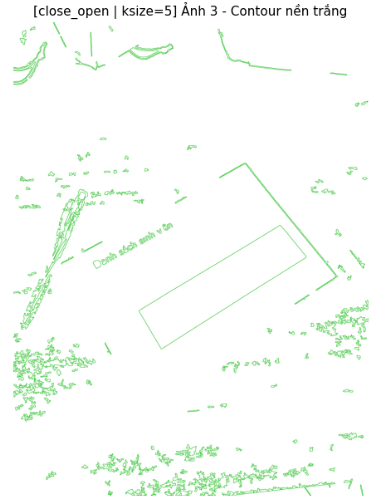
\includegraphics[width=\textwidth]{rgb_contour.png}
%         \caption{Đầu vào RGB (LAB CLAHE)}
%     \end{subfigure}
%     \hfill
%     \begin{subfigure}[b]{0.45\textwidth}
%         \centering
%         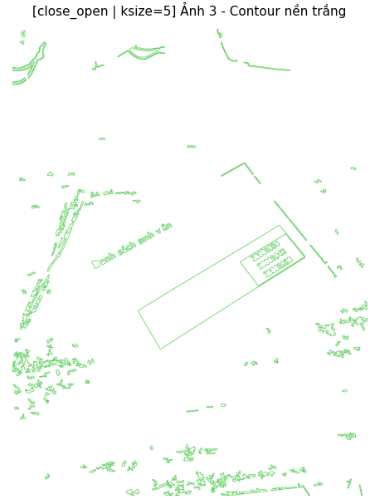
\includegraphics[width=\textwidth]{gray_contour.png}
%         \caption{Đầu vào GRAY CLAHE}
%     \end{subfigure}
%     \caption{So sánh Contour trên các hệ màu (với phép Close-Open k=5)}
%     \label{fig:color_space_contour} % Thêm label để tham chiếu
% \end{figure}

% \textbf{Nhận xét thực nghiệm và kết luận:}

% Qua Hình \ref{fig:color_space_contour}, có thể thấy ảnh RGB (LAB CLAHE) giữ được nhiều thông tin về màu sắc của nền mặt bàn, khiến thuật toán bắt nhầm các chi tiết phụ thành contour rác. Ngược lại, GRAY CLAHE chỉ còn một kênh xám, triệt tiêu được nhiễu màu và làm nổi bật sự chênh lệch cường độ sáng giữa mặt giấy và nền. Do đó, hệ thống chốt sử dụng \textbf{GRAY CLAHE kết hợp biến đổi Close rồi Open ($k=5$)} làm đầu vào tiêu chuẩn.

% \textbf{Hiệu chỉnh phối cảnh (Perspective Transform):}

% Việc dò tìm các đỉnh contour cuối cùng được thực hiện thông qua bộ lọc xấp xỉ đa giác (Polygonal Approximation). Thuật toán lọc bỏ mạnh tay các contour rác có diện tích nhỏ hoặc các bounding box không có ý nghĩa thực tế. Nhờ vậy, tọa độ 4 góc nội tiếp của tài liệu được trích xuất chính xác, sau đó ánh xạ thành ma trận điểm đích để uốn nắn hiện tượng méo do không gian chụp ba chiều gây ra.



\section{Phân đoạn ảnh}

Trong phần này chúng tôi thực hiện phân đoạn ảnh bằng các phương pháp khác nhau:
\begin{itemize}
    \item Kmean và Kmean kết hợp với tọa độ.
    \item Region Growing
    \item Watershed
\end{itemize}

Thực nghiệm trên nhiều hệ màu khác nhau như RGB, RGB được cân bằng sáng, thực hiện trên ảnh xám.

\subsection{Thuật toán Kmean và phương pháp dùng ngưỡng}

\subsubsection{Phân đoạn trên ảnh màu}

Thực nghiệm đầu tiên được tiến hành trực tiếp trên ảnh màu RGB gốc (có kết hợp bộ lọc làm nét - Sharpen).

\begin{figure}[H]
    \centering
    \begin{subfigure}[b]{\textwidth}
        \centering
        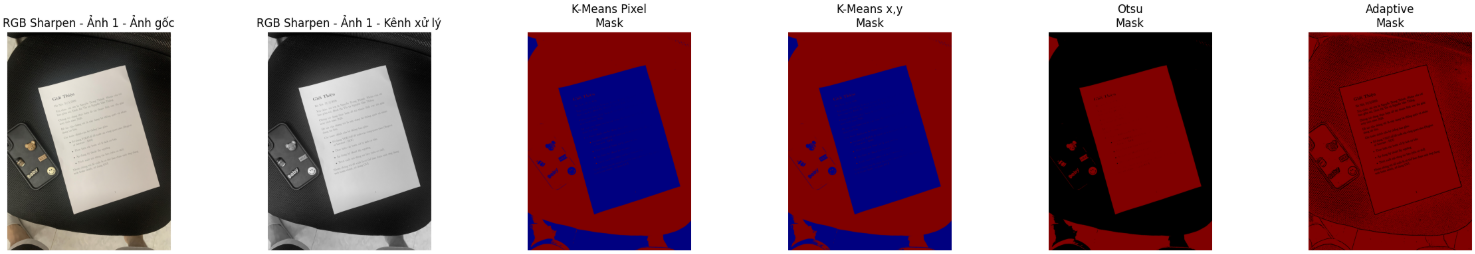
\includegraphics[width=\textwidth]{segmentation_cluster_thresh_rgb_k2.png}
        \caption{Phân đoạn với cấu hình K=2}
    \end{subfigure}
    
    \vspace{0.2cm}
    
    \begin{subfigure}[b]{\textwidth}
        \centering
        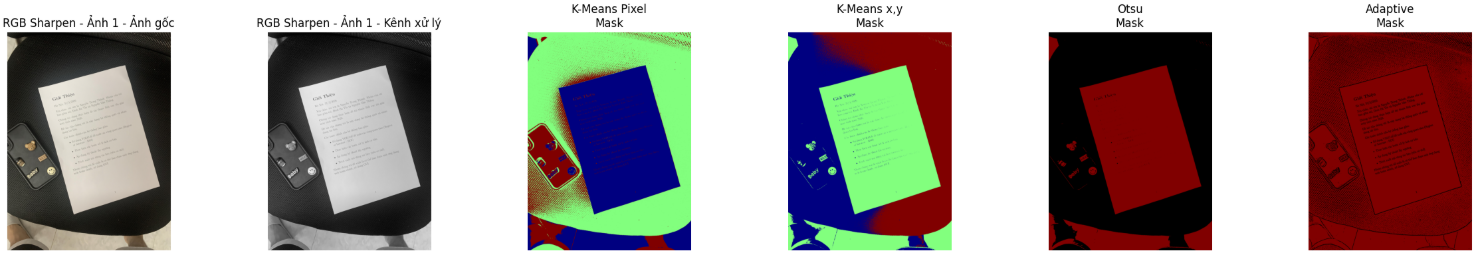
\includegraphics[width=\textwidth]{segmentation_cluster_thresh_rgb_k3.png}
        \caption{Phân đoạn với cấu hình K=3}
    \end{subfigure}
    \caption{Kết quả phân đoạn trên ảnh màu (RGB)}
\end{figure}

\textbf{Nhận xét thực nghiệm:}
\begin{itemize}
    \item \textbf{K-Means Clustering:} Cấu hình $K=2$ phân tách khá tốt vùng sáng (giấy) và tối (nền). Tuy nhiên, khi tăng lên $K=3$, thuật toán bị nhiễu bởi các đốm sáng và họa tiết nền, gây ra hiện tượng phân mảnh quá mức (Over-segmentation) làm mask kết quả bị vụn vặt.
    \item \textbf{Otsu Threshold:} Dễ bị đánh lừa bởi bóng đổ trên mặt giấy, dẫn đến việc gộp chung một phần nền tối vào tài liệu hoặc làm mất mát các vùng sáng.
    \item \textbf{Adaptive Threshold:} Làm nổi rõ nét chữ và biên giấy rất xuất sắc, nhưng lại cực kỳ nhạy cảm với nhiễu. Toàn bộ cấu trúc lưới của ghế bị bắt lại khiến mask kết quả nhiễu hạt trầm trọng.
\end{itemize}


\subsubsection{Phân đoạn trên ảnh xám}

Ảnh được chuyển sang mức xám và áp dụng cân bằng biểu đồ tần suất thích ứng (CLAHE Gray) để cải thiện độ tương phản cục bộ trước khi phân đoạn.

\begin{figure}[H]
    \centering
    \begin{subfigure}[b]{\textwidth}
        \centering
        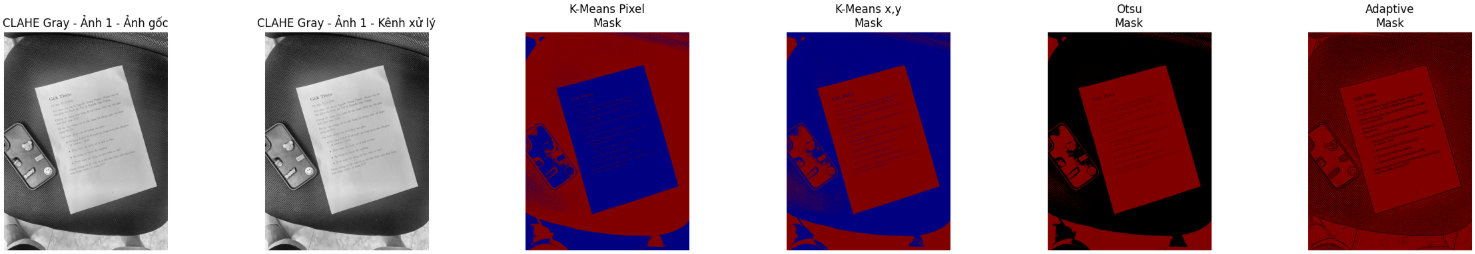
\includegraphics[width=\textwidth]{segmentation_cluster_thresh_gray_k2.png}
        \caption{Phân đoạn với cấu hình K=2}
    \end{subfigure}
    
    \vspace{0.2cm}
    
    \begin{subfigure}[b]{\textwidth}
        \centering
        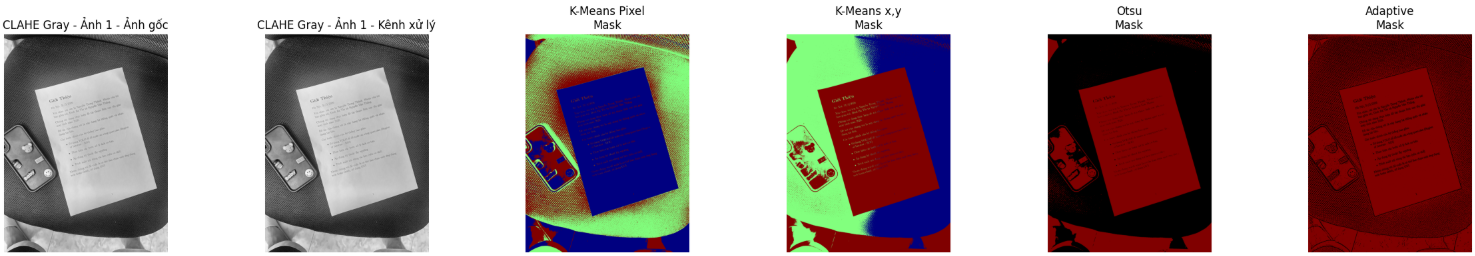
\includegraphics[width=\textwidth]{segmentation_cluster_thresh_gray_k3.png}
        \caption{Phân đoạn với cấu hình K=3}
    \end{subfigure}
    \caption{Kết quả phân đoạn trên ảnh xám (CLAHE GRAY)}
\end{figure}

\textbf{Nhận xét thực nghiệm:}
\begin{itemize}
    \item \textbf{K-Means Clustering:} Ở mức xám, $K=2$ cho thấy sự ổn định tuyệt vời, vùng giấy được cô lập gần như hoàn hảo khỏi nền mặt ghế. Trong khi đó, $K=3$ có xu hướng bóc tách riêng phần bóng đổ trên giấy thành một cụm màu thứ 3, làm mất đi tính liền mạch nguyên khối của tài liệu.
    \item \textbf{Otsu \& Adaptive Threshold:} Tương tự như trên ảnh RGB, Otsu vẫn gặp khó khăn ở các góc giấy bị tối, còn Adaptive Threshold kéo theo lượng nhiễu lớn từ texture nhám của mặt ghế.
\end{itemize}


\subsubsection{Phân đoạn trên các hệ màu khác nhau}

Để khai thác đặc tính tách biệt ánh sáng và màu sắc, hệ thống tiếp tục thử nghiệm trên hai không gian màu HSV và LAB. Cả hai đều được tiền xử lý bằng CLAHE trên kênh độ sáng tương ứng trước khi chuyển về RGB để chạy thuật toán.

\subsubsection{Phân đoạn trên hệ màu HSV}

\begin{figure}[H]
    \centering
    \begin{subfigure}[b]{\textwidth}
        \centering
        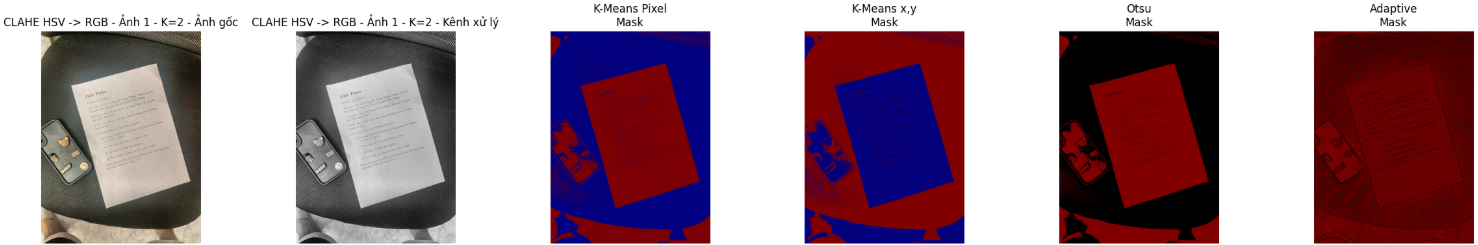
\includegraphics[width=\textwidth]{segmentation_cluster_thresh_hsv_k2.png}
        \caption{Phân đoạn với cấu hình K=2}
    \end{subfigure}
    
    \vspace{0.2cm}
    
    \begin{subfigure}[b]{\textwidth}
        \centering
        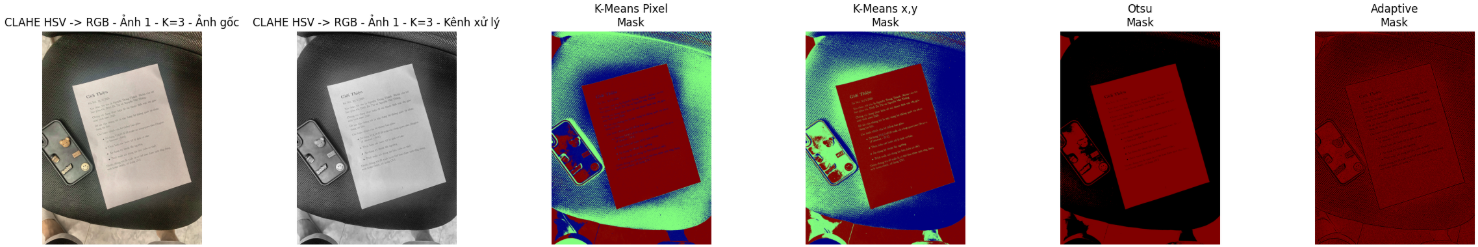
\includegraphics[width=\textwidth]{segmentation_cluster_thresh_hsv_k3.png}
        \caption{Phân đoạn với cấu hình K=3}
    \end{subfigure}
    \caption{Kết quả phân đoạn trên hệ CLAHE HSV}
\end{figure}

\textbf{Nhận xét thực nghiệm:}
Việc cân bằng sáng qua kênh V của HSV đẩy độ tương phản lên quá gắt, khiến nhiễu từ nền bị khuếch đại mạnh mẽ.
\begin{itemize}
    \item \textbf{K-Means Clustering:} Bị ảnh hưởng nặng nề bởi nhiễu. Đặc biệt ở cấu hình $K=3$, mask phân đoạn bị rối rắm và vỡ nát bởi các chi tiết phản quang li ti từ mặt ghế.
    \item \textbf{Otsu \& Adaptive Threshold:} Otsu thất bại hoàn toàn trong việc vạch ranh giới vùng tối của giấy. Adaptive Threshold bị "mù" bởi mạng lưới nhiễu rác trắng xóa bao trùm cả khung hình.
\end{itemize}

\subsubsection{Phân đoạn trên hệ màu LAB}

\begin{figure}[H]
    \centering
    \begin{subfigure}[b]{\textwidth}
        \centering
        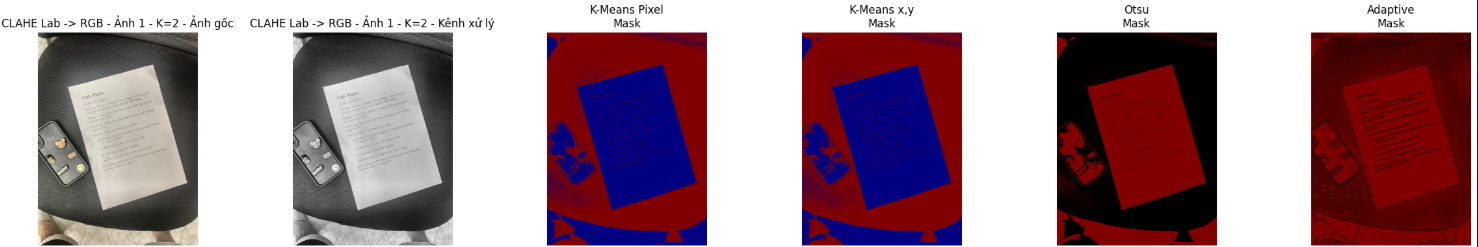
\includegraphics[width=\textwidth]{segmentation_cluster_thresh_lab_k2.png}
        \caption{Phân đoạn với cấu hình K=2}
    \end{subfigure}
    
    \vspace{0.2cm}
    
    \begin{subfigure}[b]{\textwidth}
        \centering
        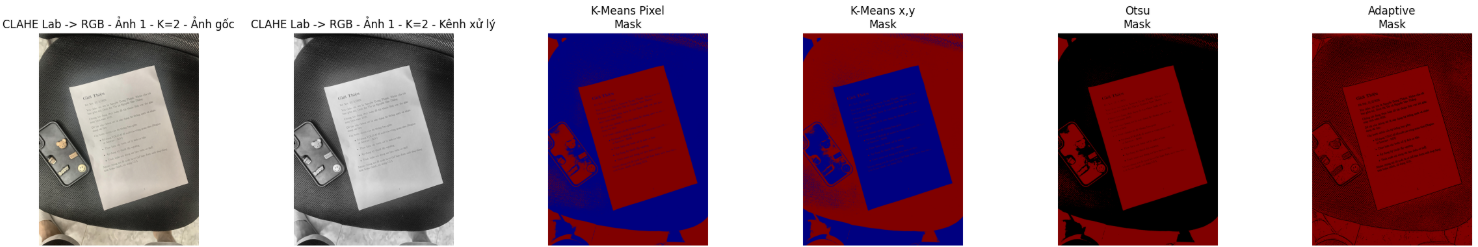
\includegraphics[width=\textwidth]{segmentation_cluster_thresh_lab_k3.png}
        \caption{Phân đoạn với cấu hình K=3}
    \end{subfigure}
    \caption{Kết quả phân đoạn trên hệ CLAHE LAB}
\end{figure}

\textbf{Nhận xét thực nghiệm:}
\begin{itemize}
    \item \textbf{Đánh giá hệ LAB:} Nhờ khả năng cô lập độ sáng (kênh L) ưu việt, LAB hạn chế được tối đa việc khuếch đại nhiễu màu so với HSV. Kết quả K-Means ($K=2$) trên hệ này cực kỳ sạch sẽ và sắc nét. Otsu cũng bắt được hình dáng tờ giấy trọn vẹn hơn.
\end{itemize}

\textbf{Kết luận tổng thể:} 
Qua thực nghiệm, Otsu bộc lộ điểm yếu khi có bóng đổ, còn Adaptive Threshold quá nhạy cảm với cấu trúc nền (texture). Do đó, phân cụm \textbf{K-Means ($K=2$)} trên \textbf{ảnh xám} hoặc hệ \textbf{LAB} là phương pháp tối ưu nhất, giúp cô lập tài liệu chính xác, ổn định và triệt tiêu nhiễu hiệu quả.vậy

\subsection{Thuật toán Watershed}

Thuật toán Watershed phân đoạn ảnh dựa trên topo học \cite{gonzalez2018}, xem cường độ sáng như các mức độ cao thấp của địa hình. Để đánh giá giới hạn của thuật toán, nhóm tiến hành thử nghiệm trên các bức ảnh có độ khó cao: \textbf{Ảnh 5} (nền bàn gỗ, nhiều đồ vật xung quanh nhưng ánh sáng khá tốt) và \textbf{Ảnh 4} (nền chăn vải có nhiều nếp gấp và họa tiết kẻ sọc phức tạp).

\subsubsection{Phân đoạn trên ảnh màu}
Bức ảnh màu gốc được áp dụng bộ lọc Sharpen để làm sắc nét biên trước khi chạy Watershed.

\begin{figure}[H]
    \centering
    \begin{subfigure}[b]{\textwidth}
        \centering
        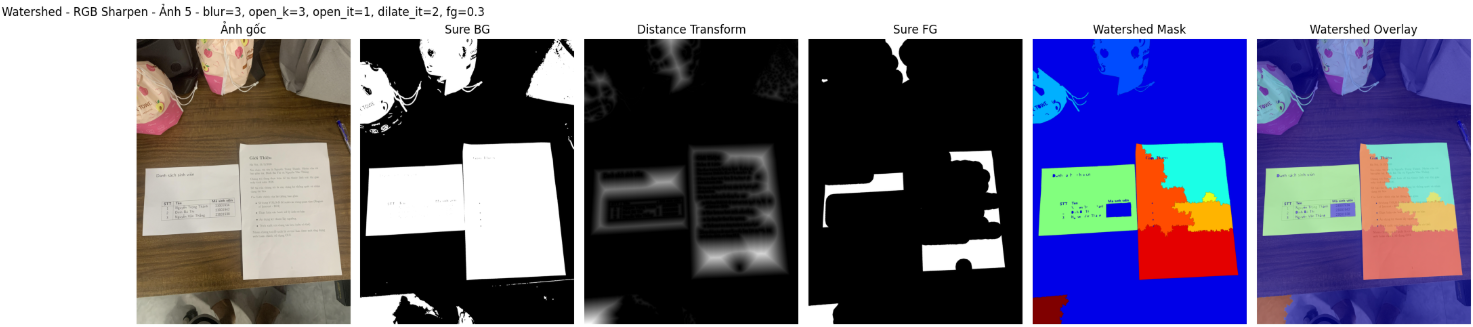
\includegraphics[width=\textwidth]{segmentation_watershed_rgb_image5_k3.png}
        \caption{Trường hợp khả quan (Ảnh 5): Tách giấy khá tốt nhưng nội bộ tờ giấy vẫn bị phân mảnh.}
    \end{subfigure}
    
    \vspace{0.3cm}
    
    \begin{subfigure}[b]{\textwidth}
        \centering
        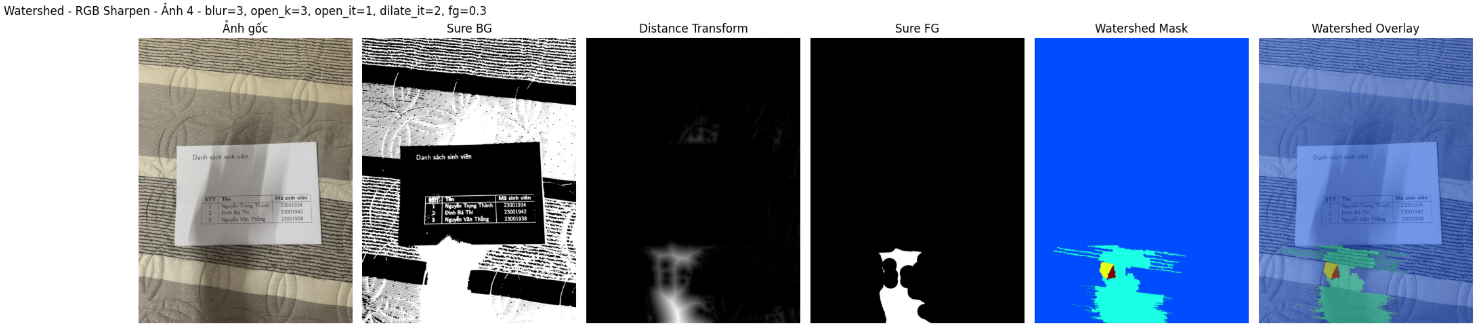
\includegraphics[width=\textwidth]{segmentation_watershed_rgb_image4_k3.png}
        \caption{Trường hợp thất bại (Ảnh 4): Marker bị xé nát do họa tiết chăn sọc và bộ lọc Sharpen.}
    \end{subfigure}
    \caption{Kết quả Watershed trên ảnh màu. Thông số: blur\_ksize=3, open\_kernel\_size=3, open\_it=1, dilate\_it=2, fg\_ratio=0.3.}
\end{figure}

\begin{figure}[H]
    \centering
    \begin{subfigure}[b]{\textwidth}
        \centering
        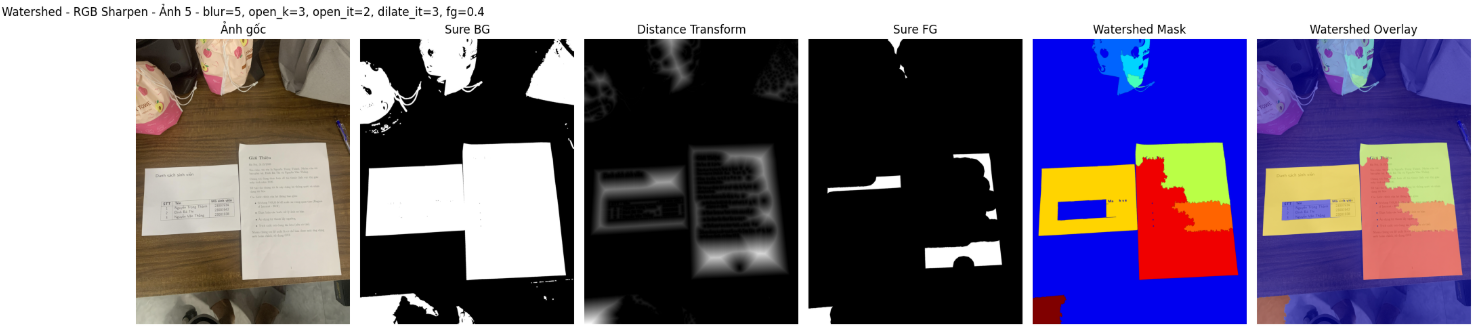
\includegraphics[width=\textwidth]{segmentation_watershed_rgb_image5_k5.png}
        \caption{Trường hợp khả quan (Ảnh 5): Tách giấy khá tốt nhưng nội bộ tờ giấy vẫn bị phân mảnh.}
    \end{subfigure}
    
    \vspace{0.3cm}
    
    \begin{subfigure}[b]{\textwidth}
        \centering
        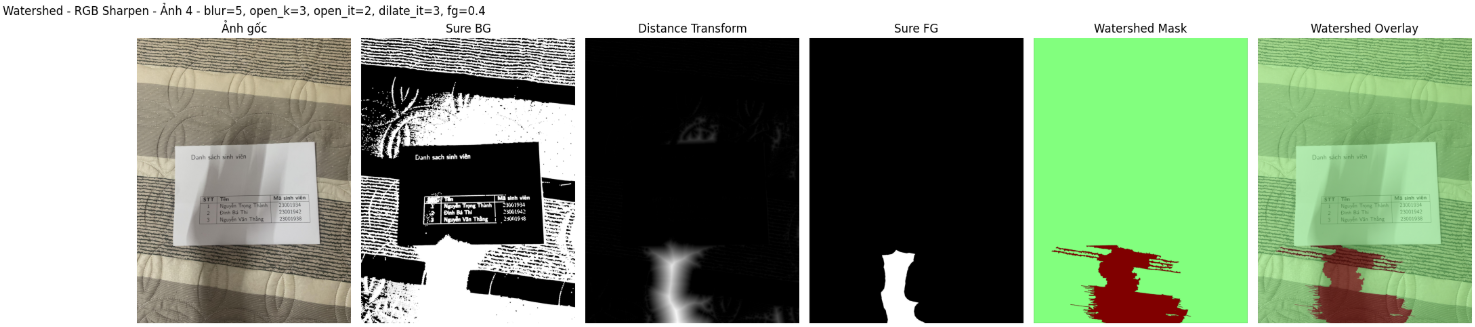
\includegraphics[width=\textwidth]{segmentation_watershed_rgb_image4_k5.png}
        \caption{Trường hợp thất bại (Ảnh 4): Marker bị xé nát do họa tiết chăn sọc và bộ lọc Sharpen.}
    \end{subfigure}
    \caption{Kết quả Watershed trên ảnh màu. Thông số: blur\_ksize=5, open\_kernel\_size=3, open\_it=2, dilate\_it=3, fg\_ratio=0.4.}
\end{figure}

\textbf{Nhận xét:} Trong khi độ tương phản tốt (Ảnh 5) giúp xác định marker (\textit{Sure FG}) chính xác và tách giấy hiệu quả, thì ở nền phức tạp (Ảnh 4), bộ lọc Sharpen lại phản tác dụng khi khuếch đại họa tiết sọc thành marker rác, khiến mask kết quả bị phân mảnh vụn vặt.

\subsubsection{Phân đoạn trên ảnh xám}
Ảnh được chuyển sang mức xám và cân bằng sáng bằng CLAHE để cải thiện độ tương phản cục bộ.

\begin{figure}[H]
    \centering
    \begin{subfigure}[b]{\textwidth}
        \centering
        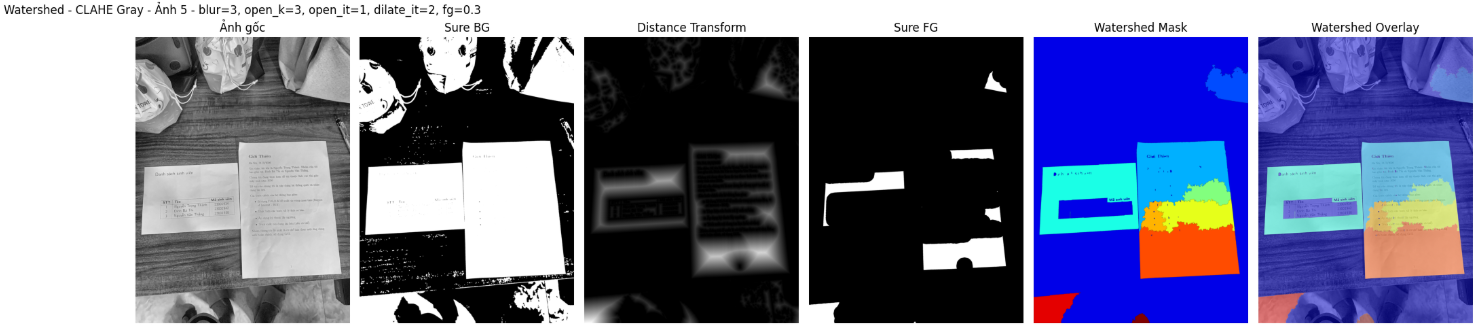
\includegraphics[width=\textwidth]{segmentation_watershed_gray_image5_k3.png}
        \caption{Trường hợp khả quan (Ảnh 5): Nền và giấy tách biệt rõ, nhưng bóng đổ chia tờ giấy làm nhiều mảng.}
    \end{subfigure}
    
    \vspace{0.3cm}
    
    \begin{subfigure}[b]{\textwidth}
        \centering
        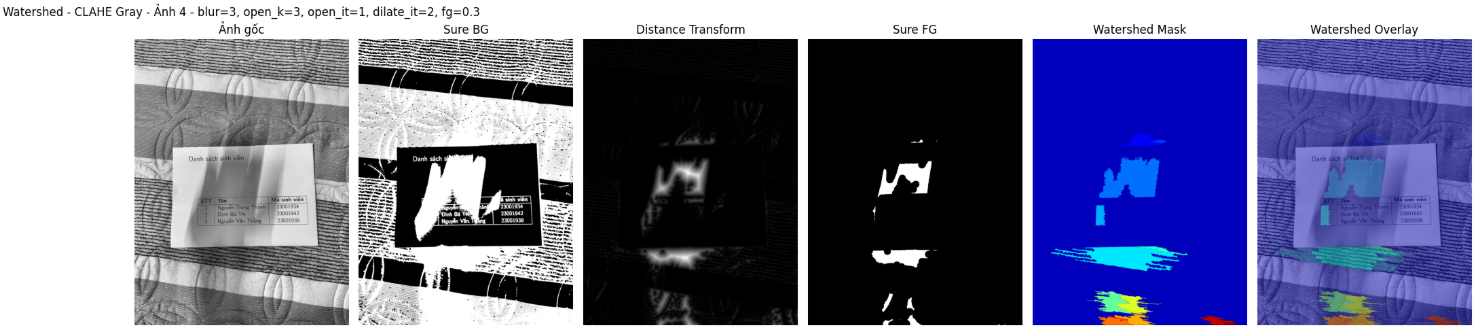
\includegraphics[width=\textwidth]{segmentation_watershed_gray_image4_k3.png}
        \caption{Trường hợp thất bại (Ảnh 4): Thuật toán hoàn toàn lúng túng trước họa tiết nền.}
    \end{subfigure}
    \caption{Kết quả Watershed trên ảnh xám(GRAY). Thông số: blur\_ksize=3, open\_kernel\_size=3, open\_it=1, dilate\_it=2, fg\_ratio=0.3.}
\end{figure}

\begin{figure}[H]
    \centering
    \begin{subfigure}[b]{\textwidth}
        \centering
        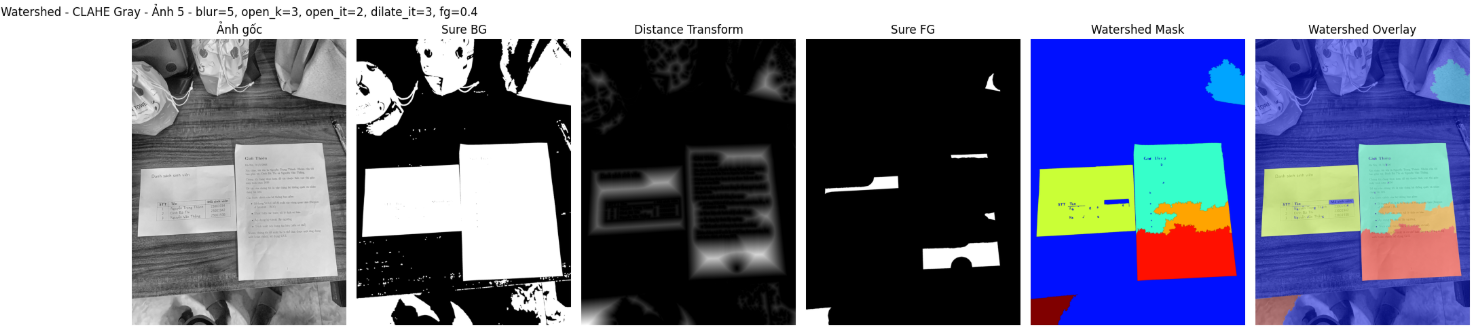
\includegraphics[width=\textwidth]{segmentation_watershed_gray_image5_k5.png}
        \caption{Trường hợp khả quan (Ảnh 5): Nền và giấy tách biệt rõ, nhưng bóng đổ chia tờ giấy làm nhiều mảng.}
    \end{subfigure}
    
    \vspace{0.3cm}
    
    \begin{subfigure}[b]{\textwidth}
        \centering
        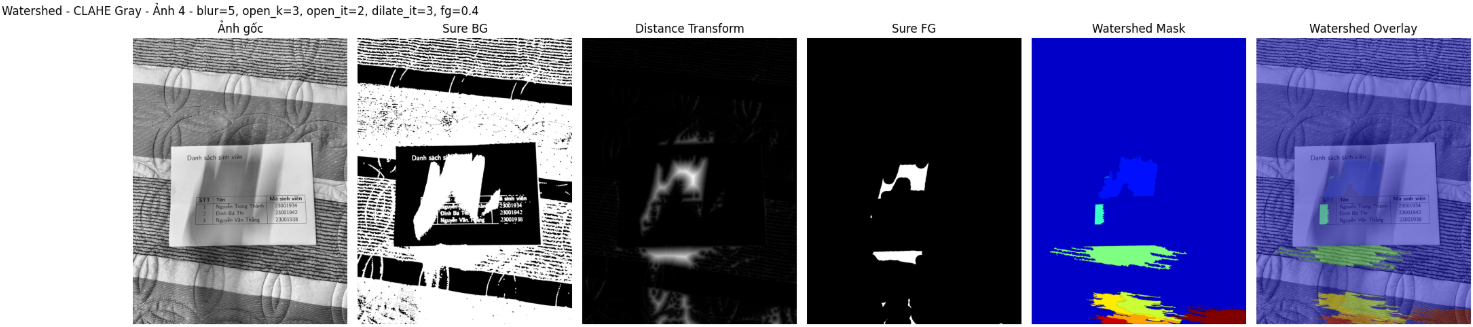
\includegraphics[width=\textwidth]{segmentation_watershed_gray_image4_k5.png}
        \caption{Trường hợp thất bại (Ảnh 4): Thuật toán hoàn toàn lúng túng trước họa tiết nền.}
    \end{subfigure}
    \caption{Kết quả Watershed trên ảnh xám(GRAY). Thông số: blur\_ksize=5, open\_kernel\_size=3, open\_it=2, dilate\_it=3, fg\_ratio=0.4.}
\end{figure}

\textbf{Nhận xét:} Mặc dù CLAHE Gray giúp khoanh vùng tài liệu rõ nét trên nền đơn giản (Ảnh 5), thuật toán lại sinh ra vô số nhiễu marker ở nền phức tạp (Ảnh 4). Nghiêm trọng hơn, các chi tiết như chữ viết và bóng đổ khiến bản thân tờ giấy bị phân mảnh quá mức (Over-segmentation), phá vỡ hoàn toàn tính nguyên khối của tài liệu.

\subsubsection{Phân đoạn trên các hệ màu khác nhau}

Nhằm khắc phục nhược điểm về bóng đổ và ánh sáng không đều của hệ Gray/RGB, nhóm mở rộng thực nghiệm sang không gian màu \textbf{HSV} và \textbf{LAB}. Việc cô lập kênh độ sáng giúp tối ưu hóa thuật toán CLAHE, từ đó hỗ trợ xác định các marker tiền cảnh và hậu cảnh chính xác hơn cho thuật toán Watershed.

\subsubsection{Phân đoạn trên hệ màu HSV}
Ảnh được chuyển sang hệ màu HSV và áp dụng thuật toán CLAHE trên kênh V (Value - cường độ sáng) nhằm tối ưu hóa việc phân tách nền trước khi chạy Watershed.

\begin{figure}[H]
    \centering
    \begin{subfigure}[b]{\textwidth}
        \centering
        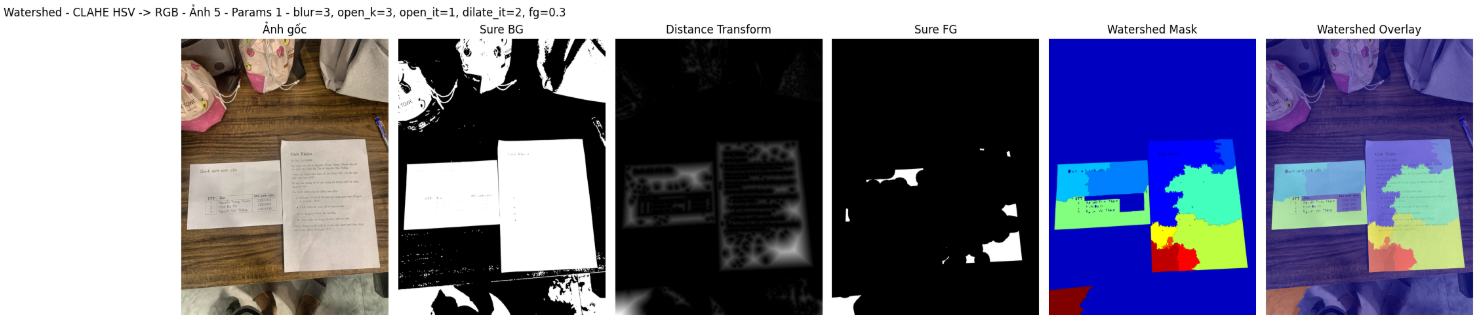
\includegraphics[width=\textwidth]{segmentation_watershed_hsv_image5_k3.png}
        \caption{Trường hợp khả quan (Ảnh 5): Tách biệt được giấy sáng màu khỏi mặt bàn.}
    \end{subfigure}
    
    \vspace{0.3cm}
    
    \begin{subfigure}[b]{\textwidth}
        \centering
        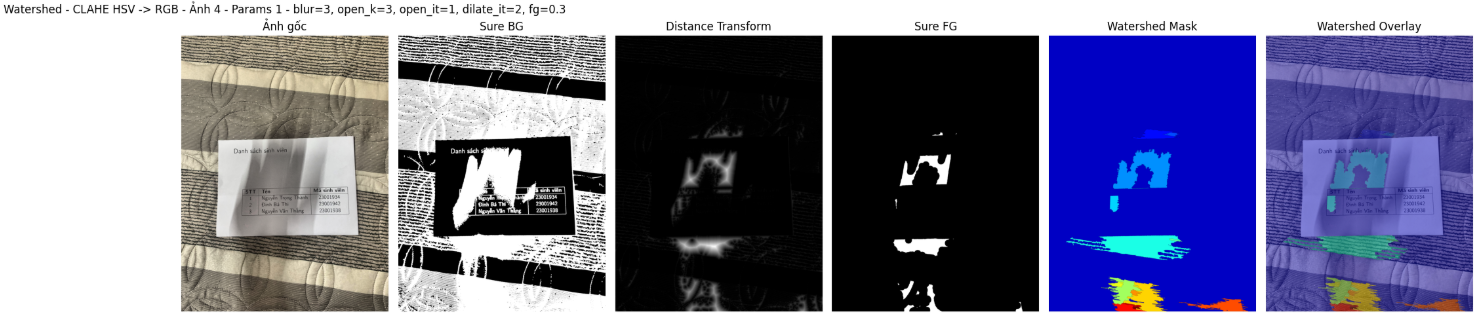
\includegraphics[width=\textwidth]{segmentation_watershed_hsv_image4_k3.png}
        \caption{Trường hợp thất bại (Ảnh 4): Marker bị nhiễu, dòng nước "lách" sai vùng.}
    \end{subfigure}
    \caption{Kết quả Watershed trên hệ màu HSV. Thông số: blur\_ksize=3, open\_kernel\_size=3, open\_it=1, dilate\_it=2, fg\_ratio=0.3.}
\end{figure}

\begin{figure}[H]
    \centering
    \begin{subfigure}[b]{\textwidth}
        \centering
        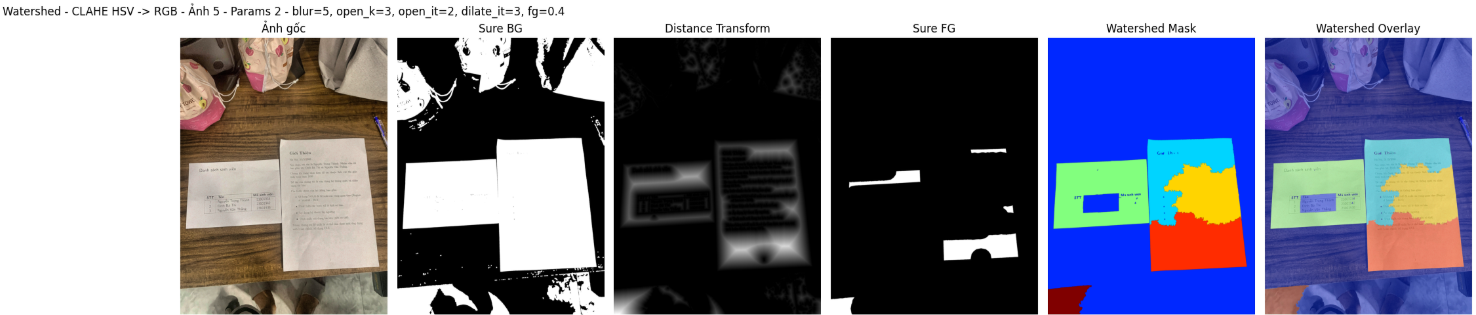
\includegraphics[width=\textwidth]{segmentation_watershed_hsv_image5_k5.png}
        \caption{Trường hợp khả quan (Ảnh 5): Tách biệt được giấy sáng màu khỏi mặt bàn.}
    \end{subfigure}
    
    \vspace{0.3cm}
    
    \begin{subfigure}[b]{\textwidth}
        \centering
        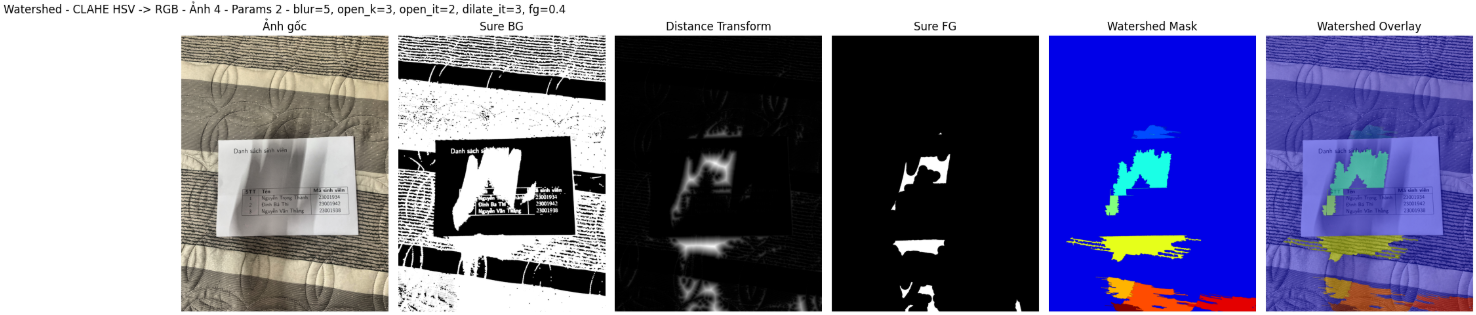
\includegraphics[width=\textwidth]{segmentation_watershed_hsv_image4_k5.png}
        \caption{Trường hợp thất bại (Ảnh 4): Marker bị nhiễu, dòng nước "lách" sai vùng.}
    \end{subfigure}
    \caption{Kết quả Watershed trên hệ màu HSV. Thông số: blur\_ksize=5, open\_kernel\_size=3, open\_it=2, dilate\_it=3, fg\_ratio=0.4.}
\end{figure}

\textbf{Nhận xét:} Kênh độ sáng của HSV giúp tách biệt tốt tài liệu khỏi các vật thể xung quanh ở điều kiện thuận lợi (Ảnh 5), nhưng vẫn không tránh khỏi việc tờ giấy bị chia nhỏ do chi tiết nội dung. Ở nền phức tạp (Ảnh 4), sự chênh lệch ánh sáng trên họa tiết gây nhiễu loạn marker, khiến dòng nước Watershed bị tràn vùng hoặc cắt lẹm vào tài liệu.


\subsubsection{Phân đoạn trên hệ màu LAB}
Sử dụng không gian màu LAB và áp dụng CLAHE trên kênh L (Lightness) để bóc tách vùng sáng tối độc lập với màu sắc.

\begin{figure}[H]
    \centering
    \begin{subfigure}[b]{\textwidth}
        \centering
        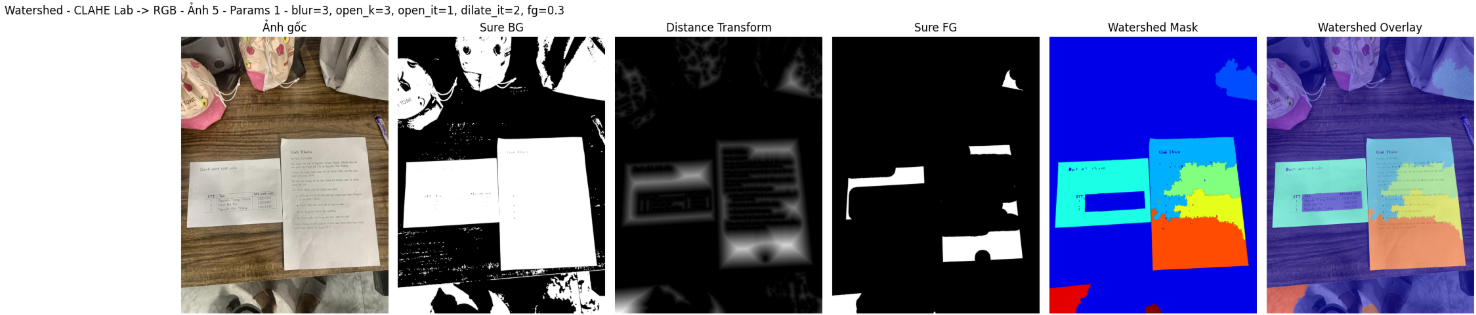
\includegraphics[width=\textwidth]{segmentation_watershed_lab_image5_k3.png}
        \caption{Trường hợp khả quan (Ảnh 5): Khoanh vùng Sure FG tương đối ổn định.}
    \end{subfigure}
    
    \vspace{0.3cm}
    
    \begin{subfigure}[b]{\textwidth}
        \centering
        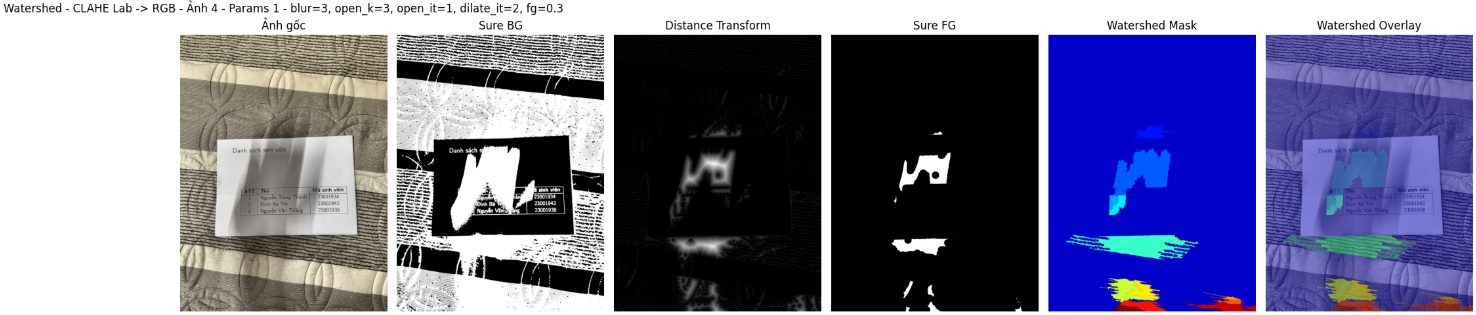
\includegraphics[width=\textwidth]{segmentation_watershed_lab_image4_k3.png} 
        \caption{Trường hợp thất bại (Ảnh 4): Cùng bộ tham số, nhưng nền vải làm mask vỡ nát.}
    \end{subfigure}
    \caption{So sánh tác động của độ phức tạp nền trên hệ màu LAB. Thông số: blur\_ksize=3, open\_kernel\_size=3, open\_it=1, dilate\_it=2, fg\_ratio=0.3.}
\end{figure}

\begin{figure}[H]
    \centering
    \begin{subfigure}[b]{\textwidth}
        \centering
        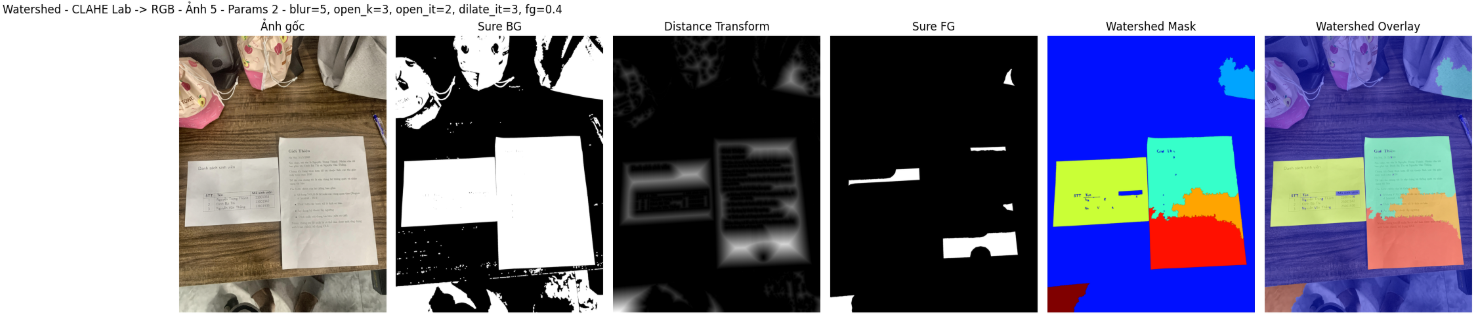
\includegraphics[width=\textwidth]{segmentation_watershed_lab_image5_k5.png}
        \caption{Trường hợp khả quan (Ảnh 5): Khoanh vùng Sure FG tương đối ổn định.}
    \end{subfigure}
    
    \vspace{0.3cm}
    
    \begin{subfigure}[b]{\textwidth}
        \centering
        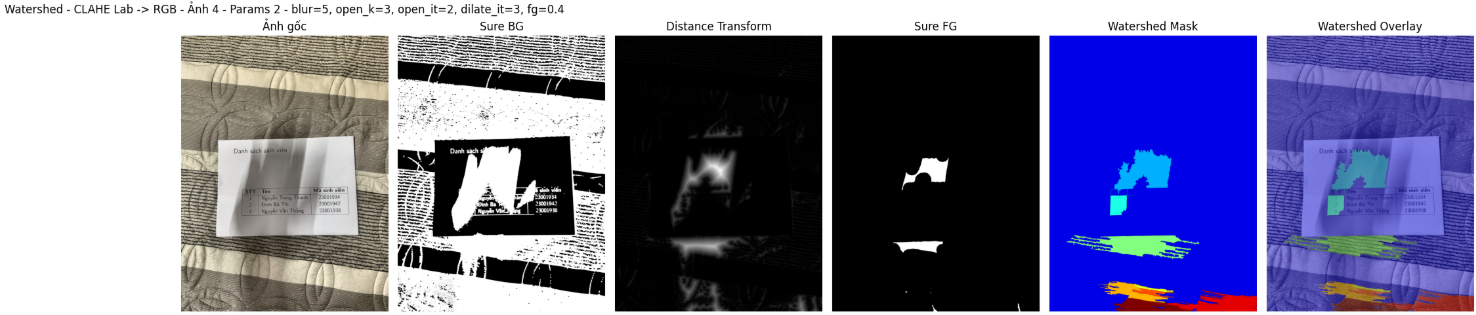
\includegraphics[width=\textwidth]{segmentation_watershed_lab_image4_k5.png} 
        \caption{Trường hợp thất bại (Ảnh 4): Cùng bộ tham số, nhưng nền vải làm mask vỡ nát.}
    \end{subfigure}
    \caption{So sánh tác động của độ phức tạp nền trên hệ màu LAB. Thông số: blur\_ksize=5, open\_kernel\_size=3, open\_it=2, dilate\_it=3, fg\_ratio=0.4.}
\end{figure}

\textbf{Nhận xét:} Tương tự HSV, hệ LAB phát hiện vùng giấy dứt khoát nhờ khả năng cô lập độ sáng tốt (Ảnh 5), song vẫn không tránh khỏi lỗi phân mảnh nội bộ do chi tiết văn bản. Với nền vải họa tiết (Ảnh 4), thuật toán hoàn toàn thất bại khi các bước sinh marker bị đứt gãy, dẫn đến mask phân đoạn vỡ nát và làm mất cấu trúc tứ giác nguyên bản của tài liệu.

\subsubsection{Nhận xét tổng thể}
Mặc dù Watershed có khả năng tách các vật thể dính liền, nó không thực sự phù hợp cho bài toán scan tài liệu. Bản chất tài liệu chứa chữ viết và bóng đổ khiến Watershed quá nhạy cảm, dẫn đến hiện tượng phân mảnh quá mức (Over-segmentation). Việc tinh chỉnh tham số không thể giải quyết triệt để sự lộn xộn này, làm mất định dạng tứ giác cần thiết cho các bước xử lý sau.



\subsection{Thuật toán Region Growing}

Ngược lại với Watershed, Region Growing phân đoạn ảnh bằng cách lan truyền vùng từ các điểm mầm được chọn trước dựa trên tiêu chí đồng nhất màu sắc hoặc cường độ \cite{gonzalez2018}. Trong thực nghiệm, thuật toán sử dụng liên kết 8-láng giềng và cơ chế cập nhật trung bình vùng động, giúp vùng phát triển liên tục hơn và thích nghi tốt hơn với các thay đổi sáng tối trên bề mặt giấy.

Các thử nghiệm được thực hiện với nhiều vị trí điểm mầm khác nhau, gồm điểm trung tâm, điểm góc tư và kết hợp nhiều điểm mầm. Đồng thời, hai mức ngưỡng \texttt{T=20} và \texttt{T=60} được khảo sát để đánh giá ảnh hưởng đến kết quả phân đoạn.

Tuy nhiên, Region Growing có chi phí tính toán lớn do phải duyệt từng pixel và kiểm tra các láng giềng. Với ảnh độ phân giải cao, thuật toán chạy chậm và dễ gây tràn bộ nhớ, nên thực nghiệm được giới hạn trên số lượng ảnh nhỏ hơn để bảo đảm quá trình xử lý hoàn tất.


\subsubsection{Phân đoạn trên ảnh màu}

\begin{figure}[H]
    \centering
    \begin{subfigure}[b]{\textwidth}
        \centering
        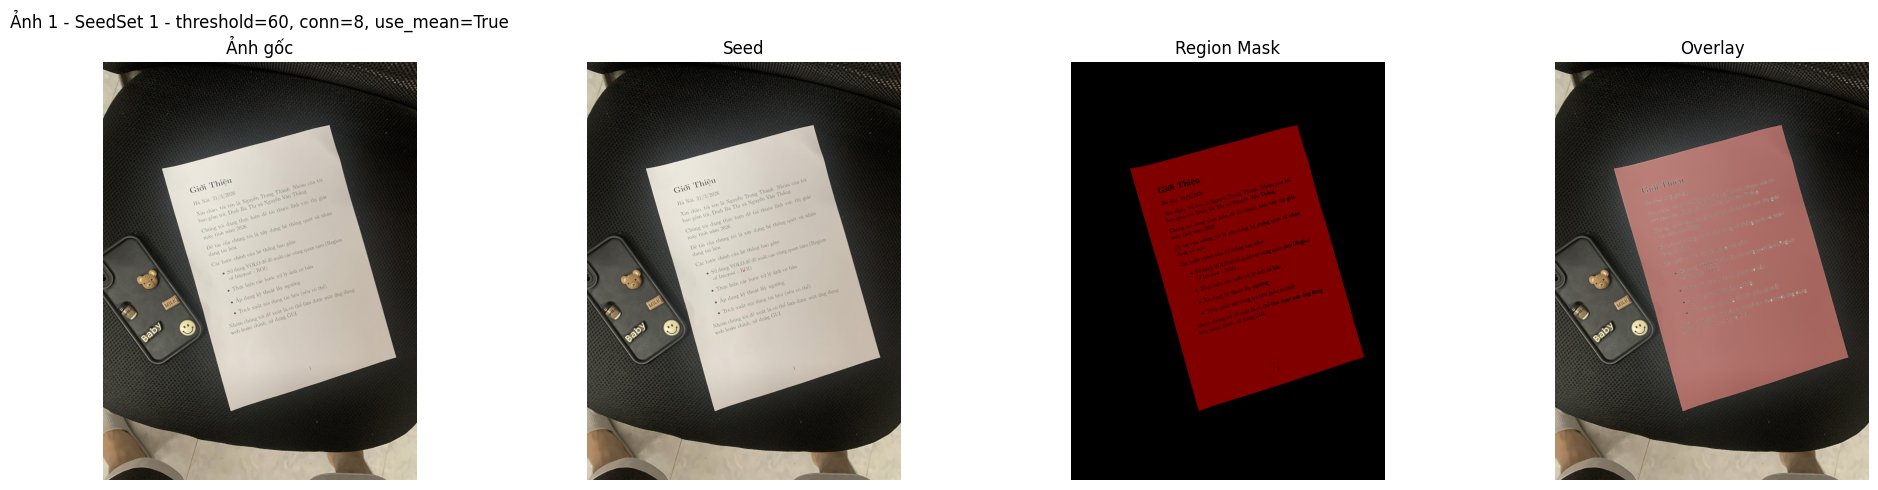
\includegraphics[width=\textwidth]{region1_60.png}
        \caption{Ảnh 1 - Seed tại tâm ảnh, \texttt{threshold=60}, \texttt{conn=8}, \texttt{use\_mean=True}}
    \end{subfigure}

    \vspace{0.2cm}

    \begin{subfigure}[b]{\textwidth}
        \centering
        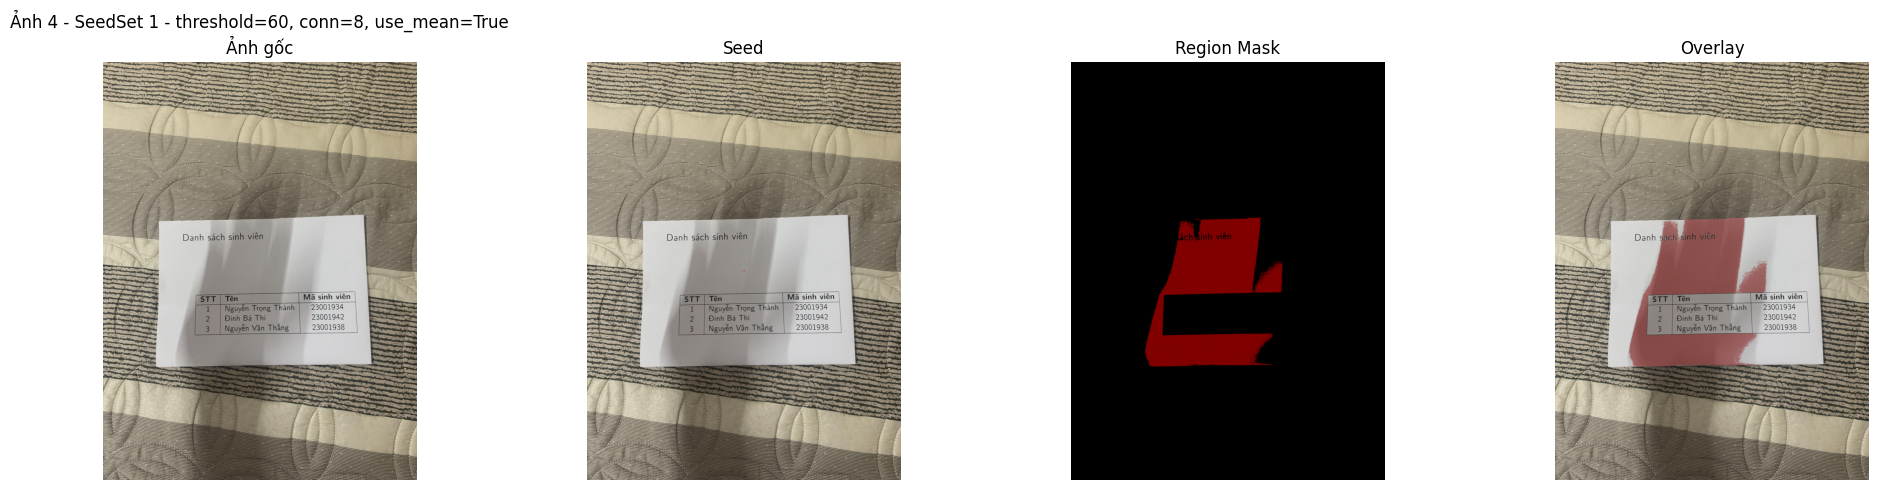
\includegraphics[width=\textwidth]{region2_60.png}
        \caption{Ảnh 2 - Seed tại tâm ảnh, \texttt{threshold=60}, \texttt{conn=8}, \texttt{use\_mean=True}}
    \end{subfigure}

    \caption{Kết quả Region Growing với ngưỡng \texttt{threshold=60} trên các ảnh thử nghiệm}
    \label{fig:region-growing-60-part1}
\end{figure}

\begin{figure}[H]
    \centering
    \begin{subfigure}[b]{\textwidth}
        \centering
        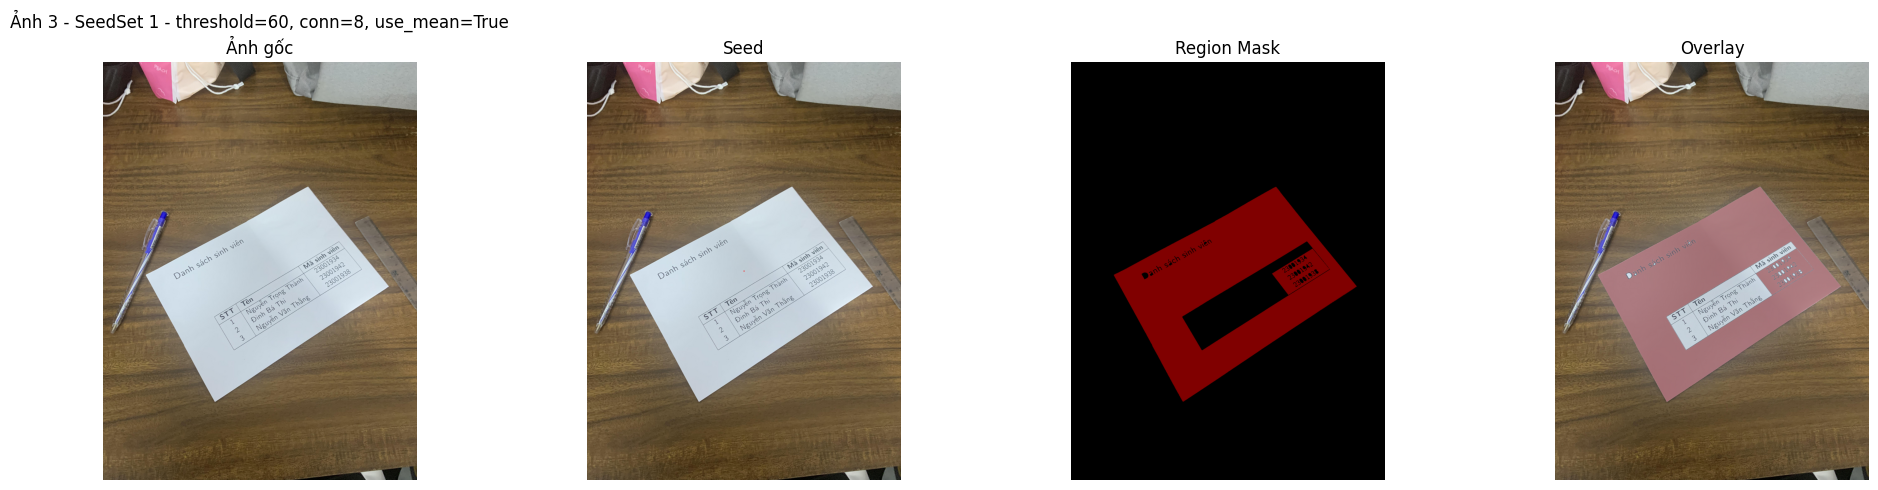
\includegraphics[width=\textwidth]{region3_60.png}
        \caption{Ảnh 3 - Seed tại tâm ảnh, \texttt{threshold=60}, \texttt{conn=8}, \texttt{use\_mean=True}}
    \end{subfigure}

    \vspace{0.2cm}

    \begin{subfigure}[b]{\textwidth}
        \centering
        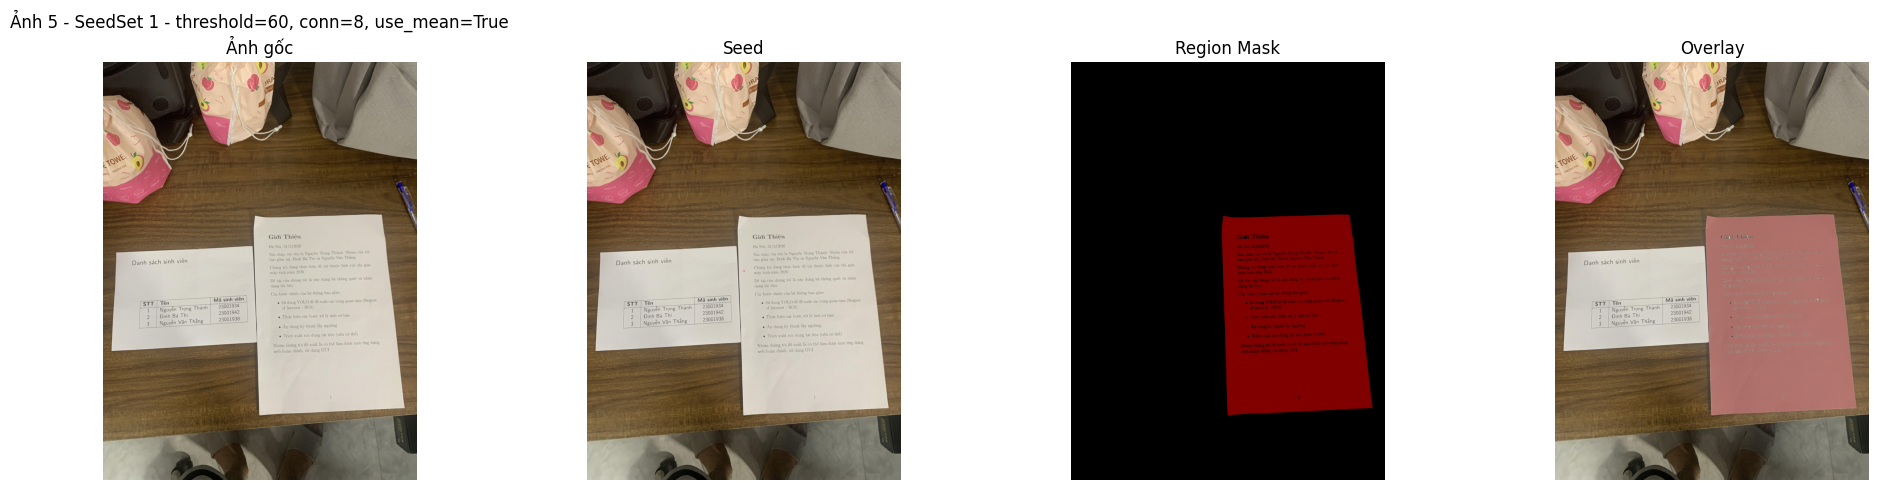
\includegraphics[width=\textwidth]{region4_60.png}
        \caption{Ảnh 4 - Seed tại tâm ảnh, \texttt{threshold=60}, \texttt{conn=8}, \texttt{use\_mean=True}}
    \end{subfigure}

    \caption{Kết quả Region Growing với ngưỡng \texttt{threshold=60} trên các ảnh thử nghiệm}
    \label{fig:region-growing-60-part2}
\end{figure}

Với cấu hình \texttt{T=60} và seed đặt tại trung tâm, Region Growing có thể lan truyền tốt trên vùng giấy có màu tương đối đồng nhất. Ở các ảnh nền đơn giản và độ tương phản giữa giấy với nền rõ, vùng tài liệu được tách khá đầy đủ. Tuy nhiên, khi trên giấy có bóng đổ, chữ đậm hoặc bảng biểu, thuật toán dễ bị ngắt vùng hoặc bỏ sót một số khu vực do sự thay đổi cường độ lớn.

\subsubsection{Phân đoạn trên ảnh xám}
\begin{figure}[H]
    \centering

    \begin{subfigure}{\textwidth}
        \centering
        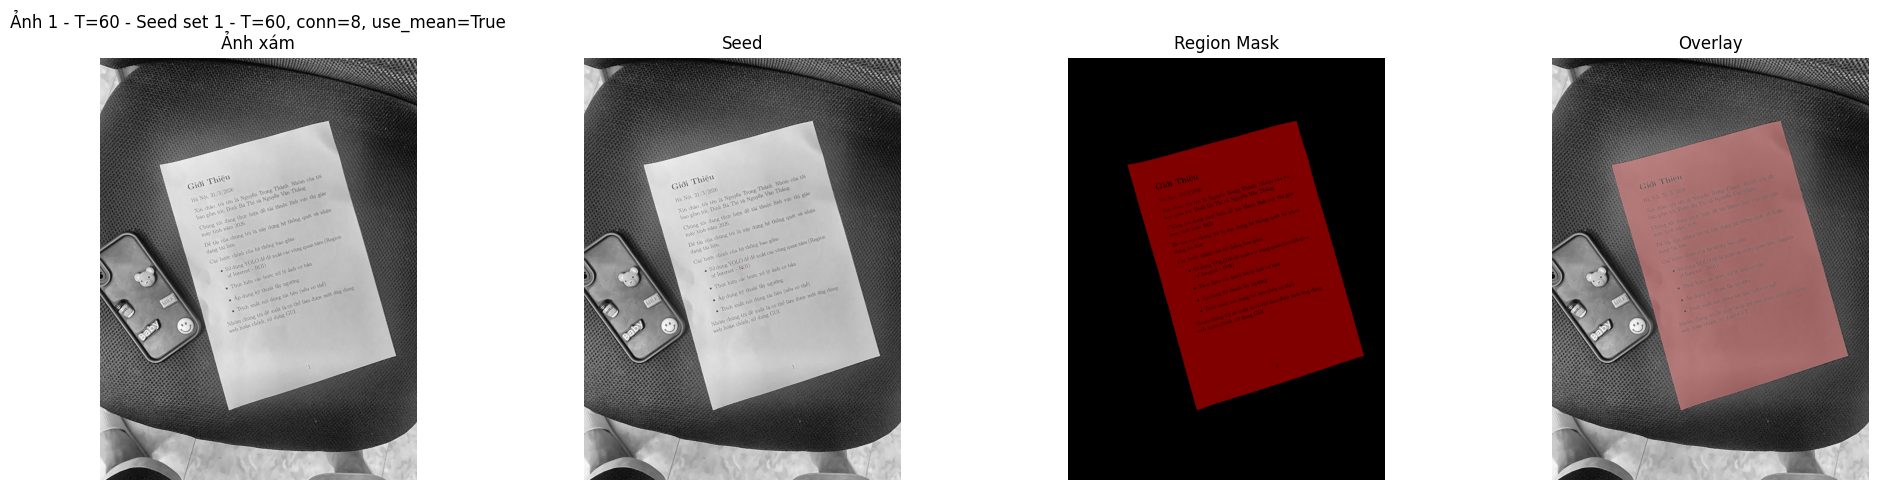
\includegraphics[width=\textwidth]{region_gray_1_60.png}
        \caption{Ảnh 1}
    \end{subfigure}

    \vspace{0.3cm}

    \begin{subfigure}{\textwidth}
        \centering
        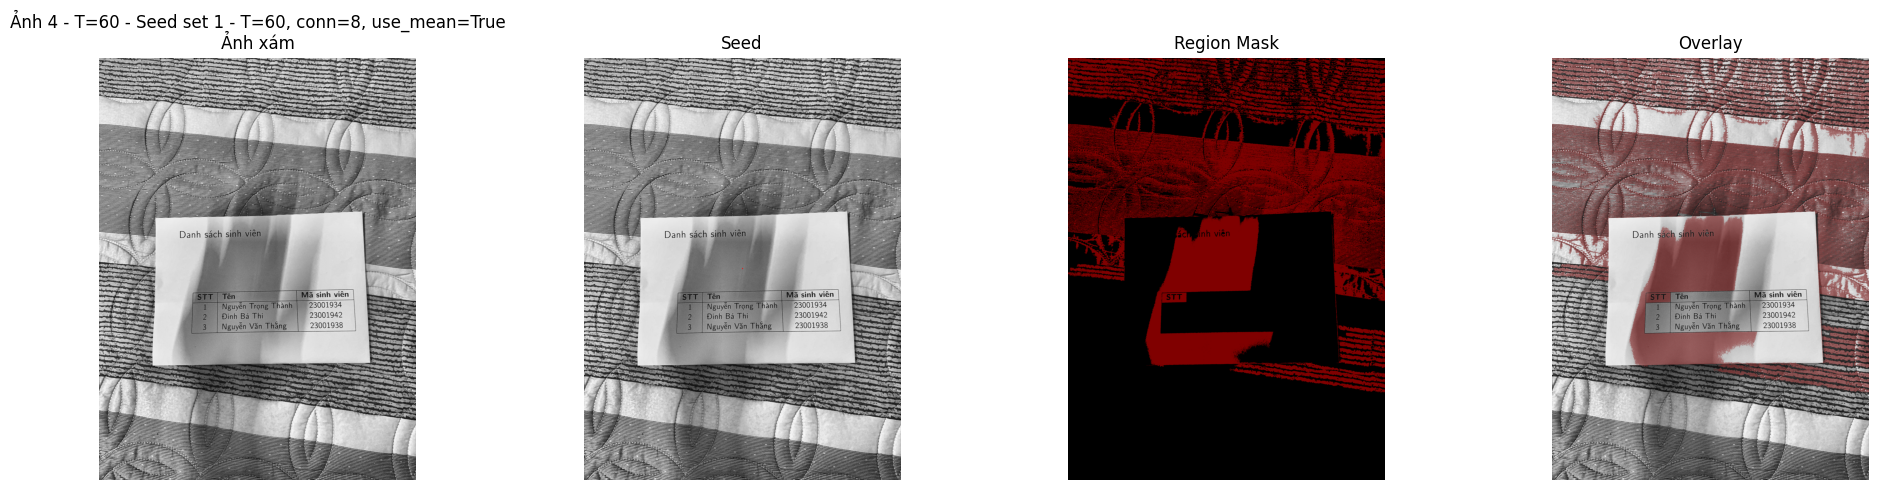
\includegraphics[width=\textwidth]{region_gray_2_60.png}
        \caption{Ảnh 5}
    \end{subfigure}

    \vspace{0.3cm}

    \begin{subfigure}{\textwidth}
        \centering
        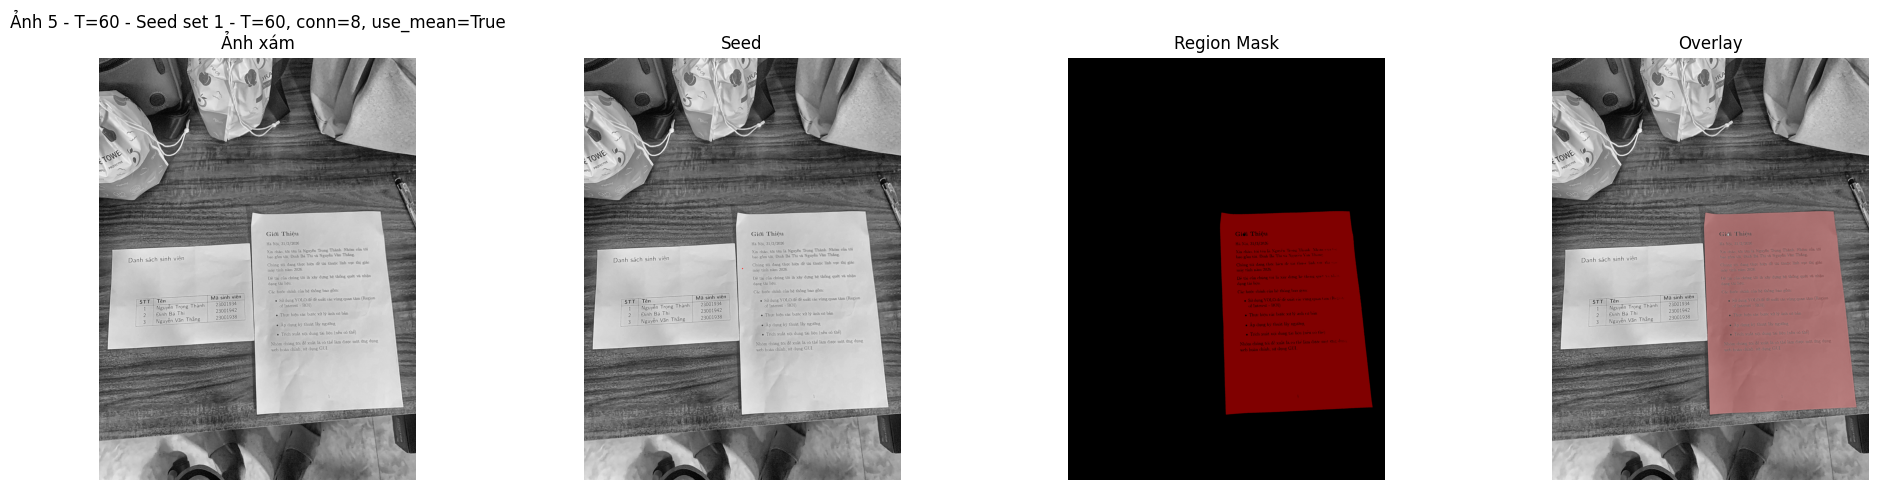
\includegraphics[width=\textwidth]{region_gray_3_60.png}
        \caption{Ảnh 4}
    \end{subfigure}

    \vspace{0.3cm}

    \begin{subfigure}{\textwidth}
        \centering
        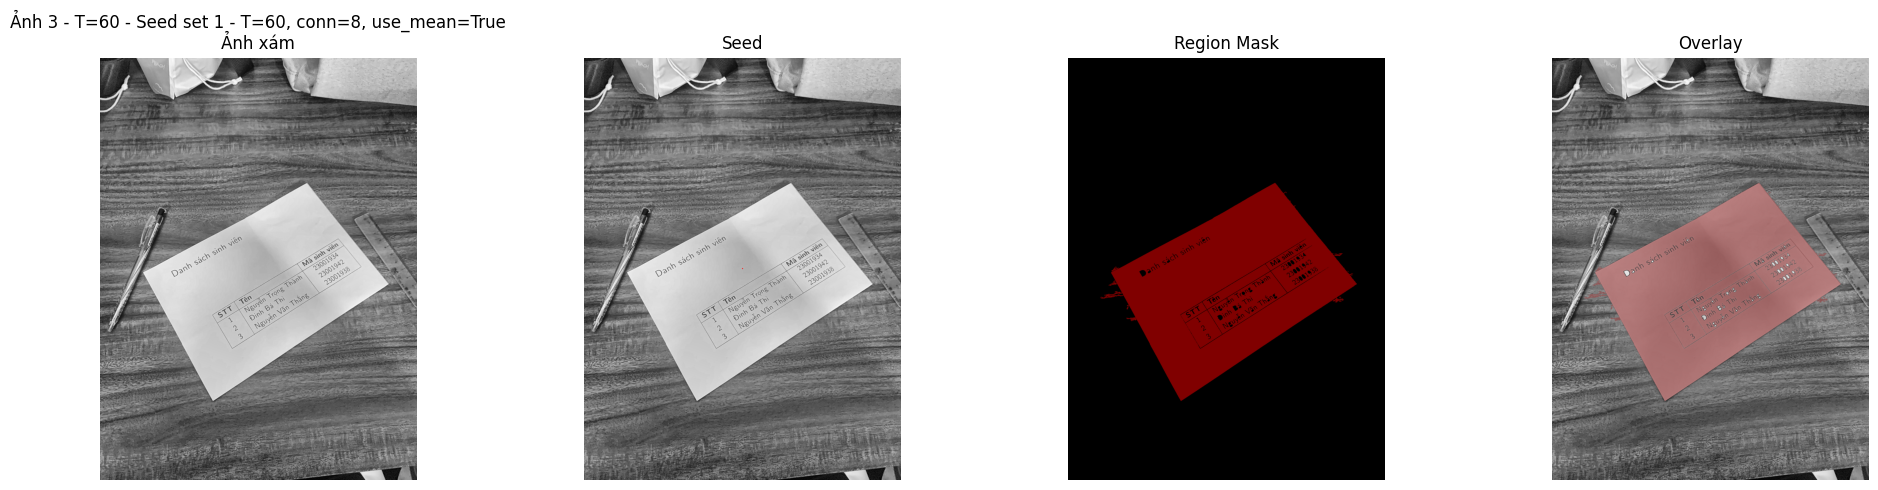
\includegraphics[width=\textwidth]{region_gray_4_60.png}
        \caption{Ảnh 3}
    \end{subfigure}

    \caption{Một số kết quả Region Growing trên ảnh xám với ngưỡng $T = 60$.}
    \label{fig:region-growing-gray-t60}
\end{figure}


Với ngưỡng $T = 60$, Region Growing trên ảnh xám hoạt động tốt khi tài liệu có độ tương phản rõ với nền. Ngược lại, nếu nền phức tạp hoặc mức xám gần giống tài liệu, vùng phân đoạn dễ bị lan sang nền hoặc thiếu chính xác.

\subsubsection{Phân đoạn trên các hệ màu khác}

Với ảnh  RGB được cân bằng sáng trên HSV

\begin{figure}[H]
    \centering

    \begin{subfigure}{\textwidth}
        \centering
        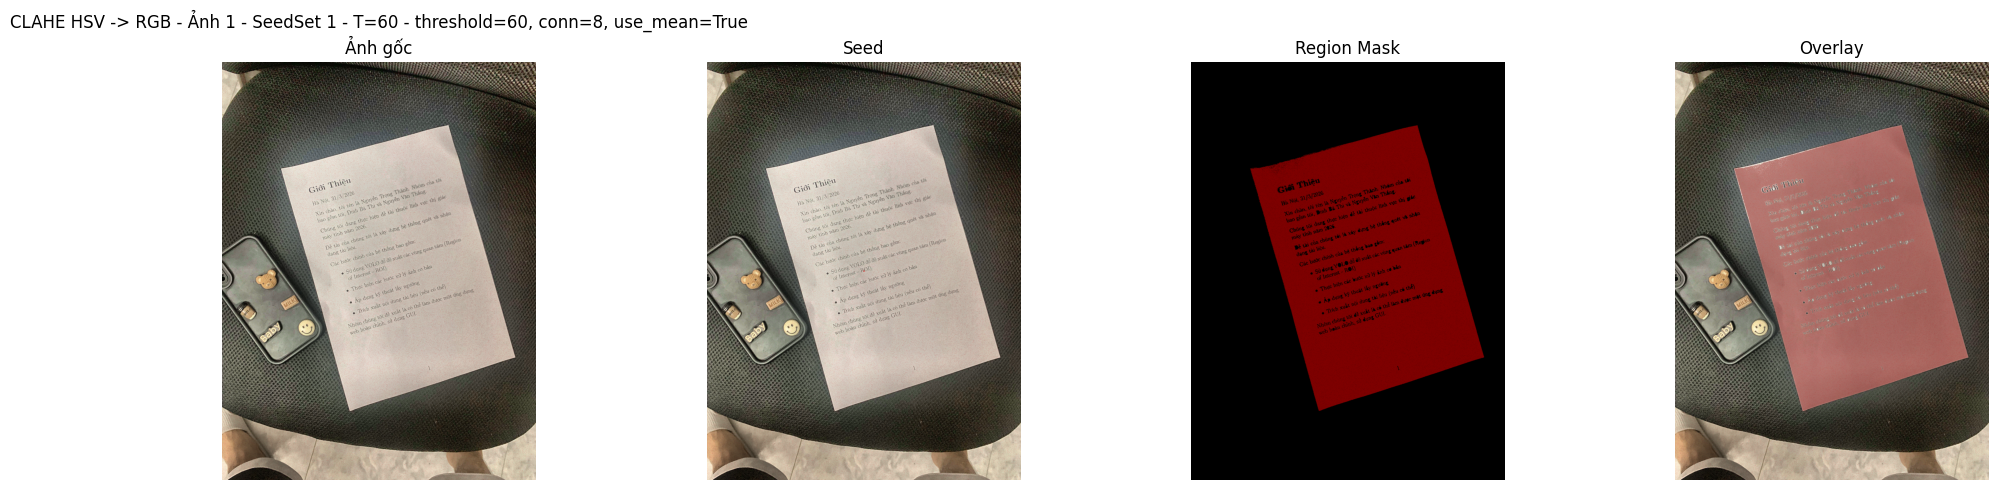
\includegraphics[width=\textwidth]{region_hsv_1_60.png}
        \caption{Ảnh 1}
    \end{subfigure}

    \vspace{0.3cm}

    \begin{subfigure}{\textwidth}
        \centering
        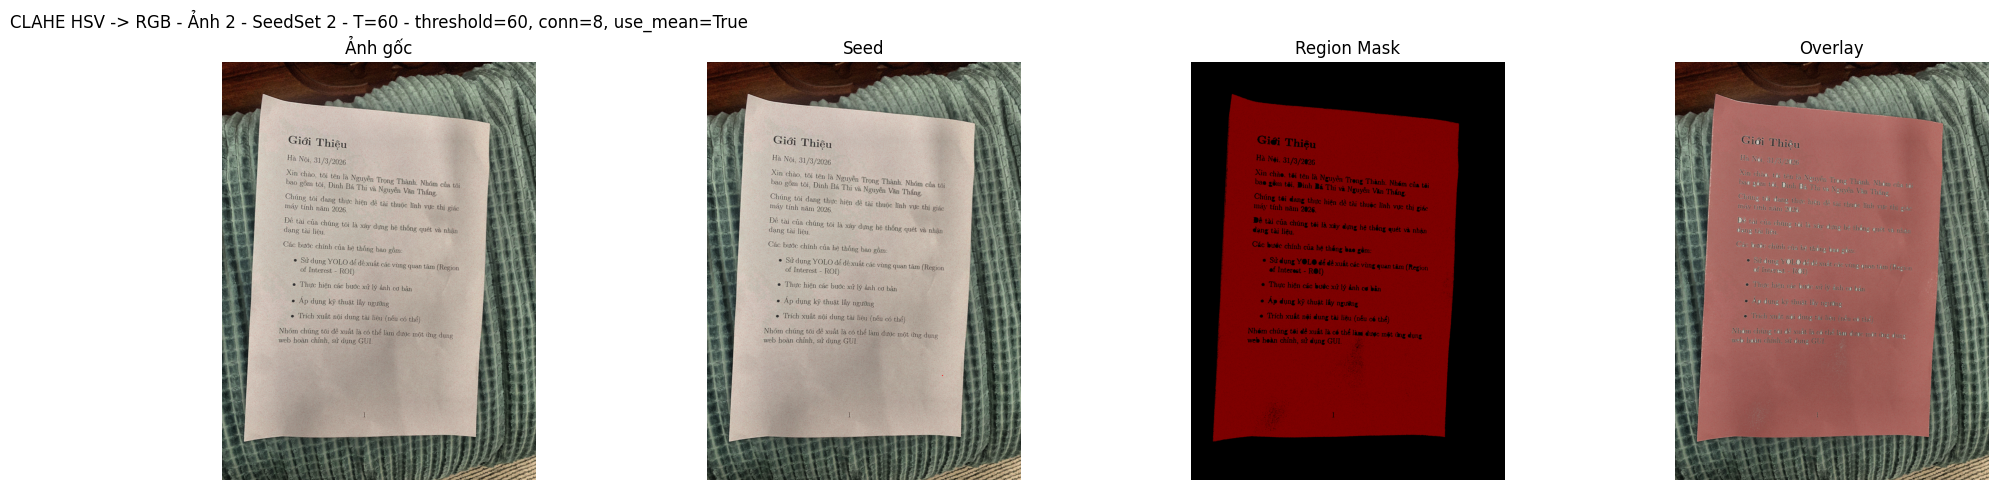
\includegraphics[width=\textwidth]{region_hsv_2_60.png}
        \caption{Ảnh 2}
    \end{subfigure}

    \caption{So sánh kết quả Region Growing trên ảnh RGB sau khi cân bằng sáng trên không gian màu HSV với ngưỡng $T = 60$.}
    \label{fig:region-growing-hsv-t60}
\end{figure}


Còn đối với ảnh được cân bằng sáng trên không gian màu LAB.


\begin{figure}[H]
    \centering

    \begin{subfigure}{\textwidth}
        \centering
        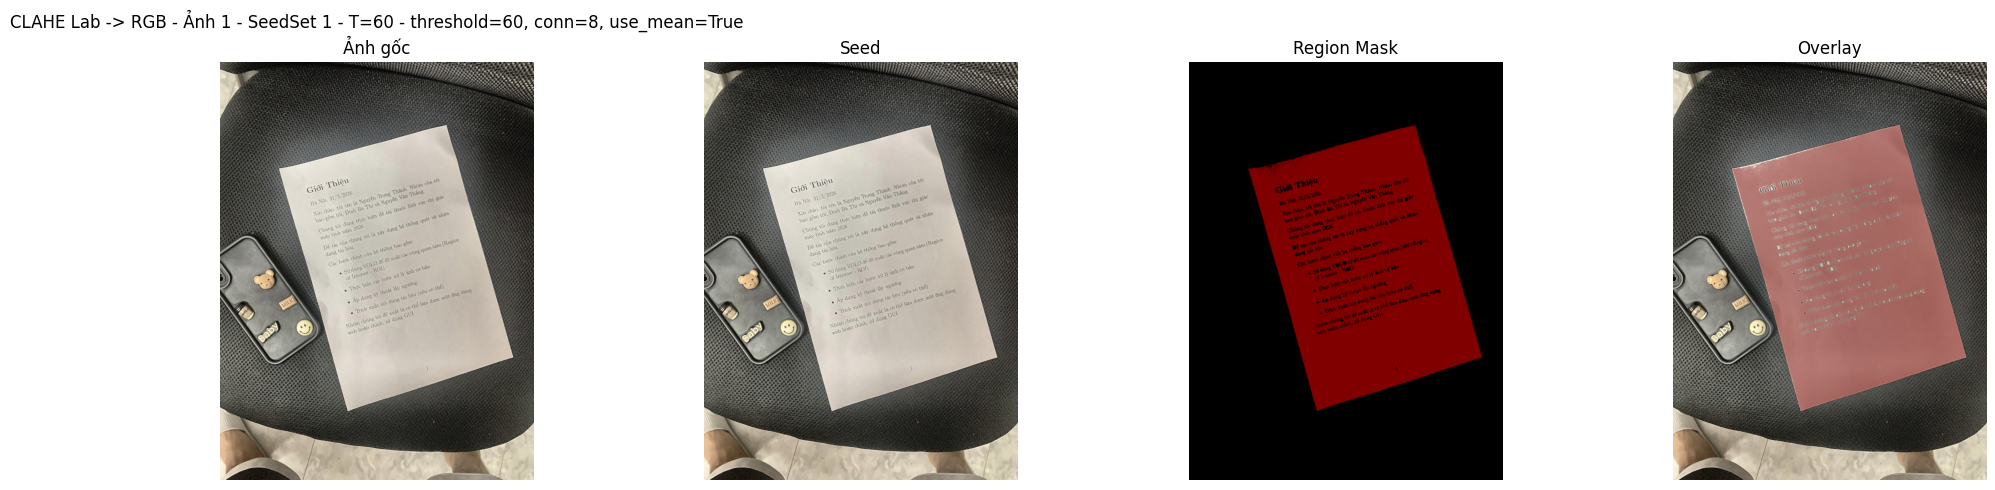
\includegraphics[width=\textwidth]{region_lab_1_60.png}
        \caption{Ảnh 1}
    \end{subfigure}

    \vspace{0.3cm}

    \begin{subfigure}{\textwidth}
        \centering
        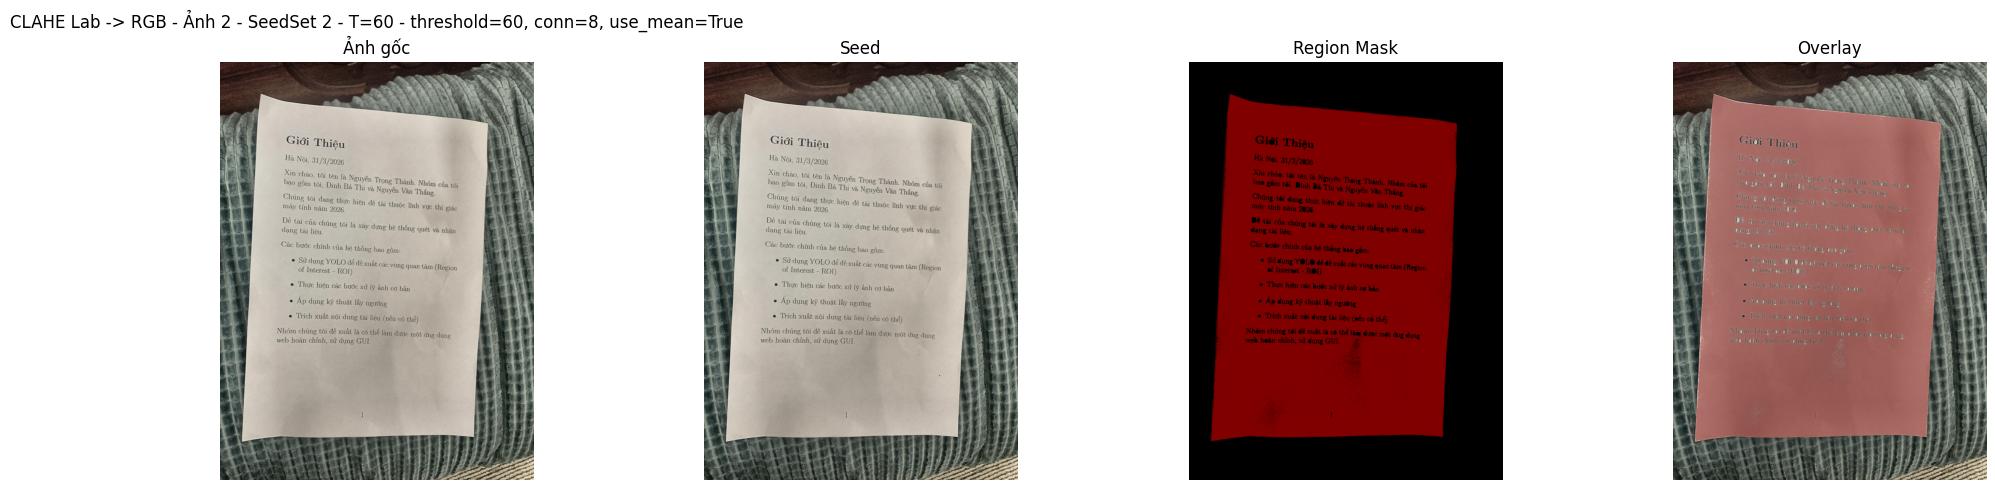
\includegraphics[width=\textwidth]{region_lab_2_60.png}
        \caption{Ảnh 2}
    \end{subfigure}

    \caption{So sánh kết quả Region Growing trên ảnh RGB sau khi cân bằng sáng trên không gian màu LAB với ngưỡng $T = 60$.}
    \label{fig:region-growing-lab-t60}
\end{figure}



\subsubsection{Ảnh hưởng của ngưỡng}

\begin{figure}[H]
    \centering
    
    \begin{subfigure}[b]{\textwidth}
        \centering
        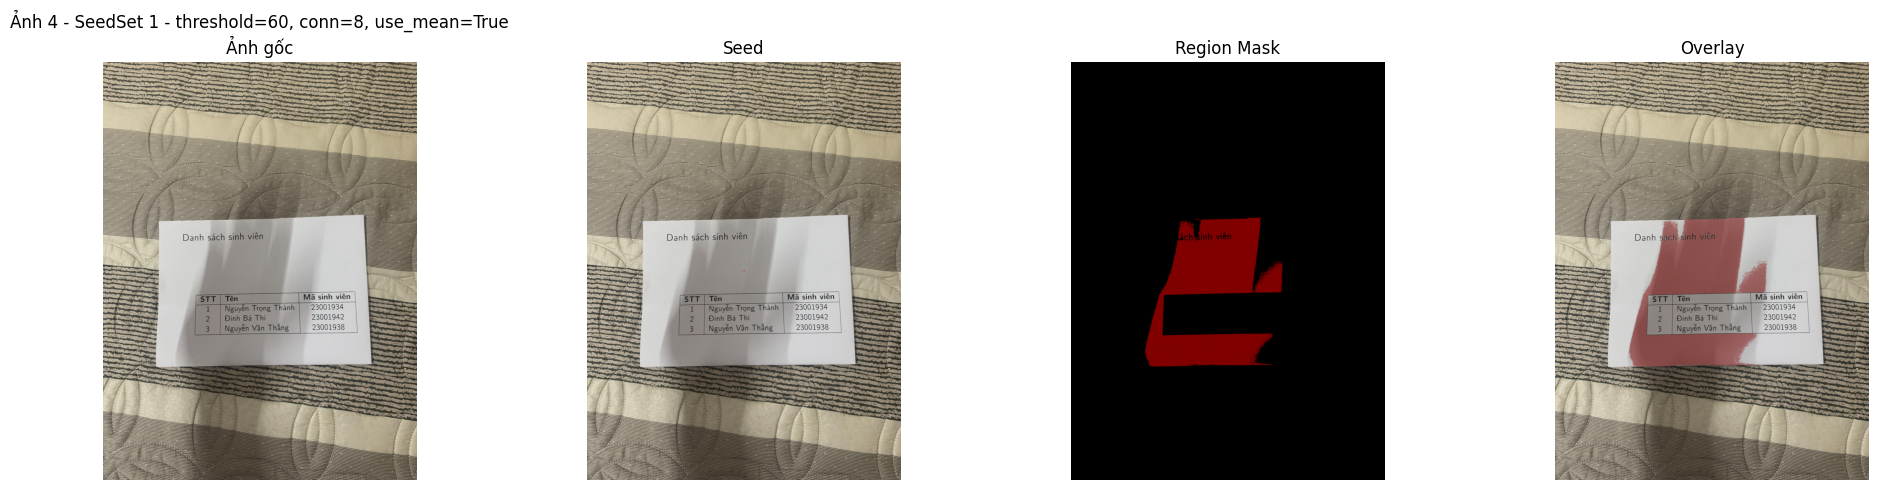
\includegraphics[width=\textwidth]{region2_60.png}
        \caption{Ảnh 4 với \texttt{threshold=60}}
    \end{subfigure}

    \vspace{0.2cm}

    \begin{subfigure}[b]{\textwidth}
        \centering
        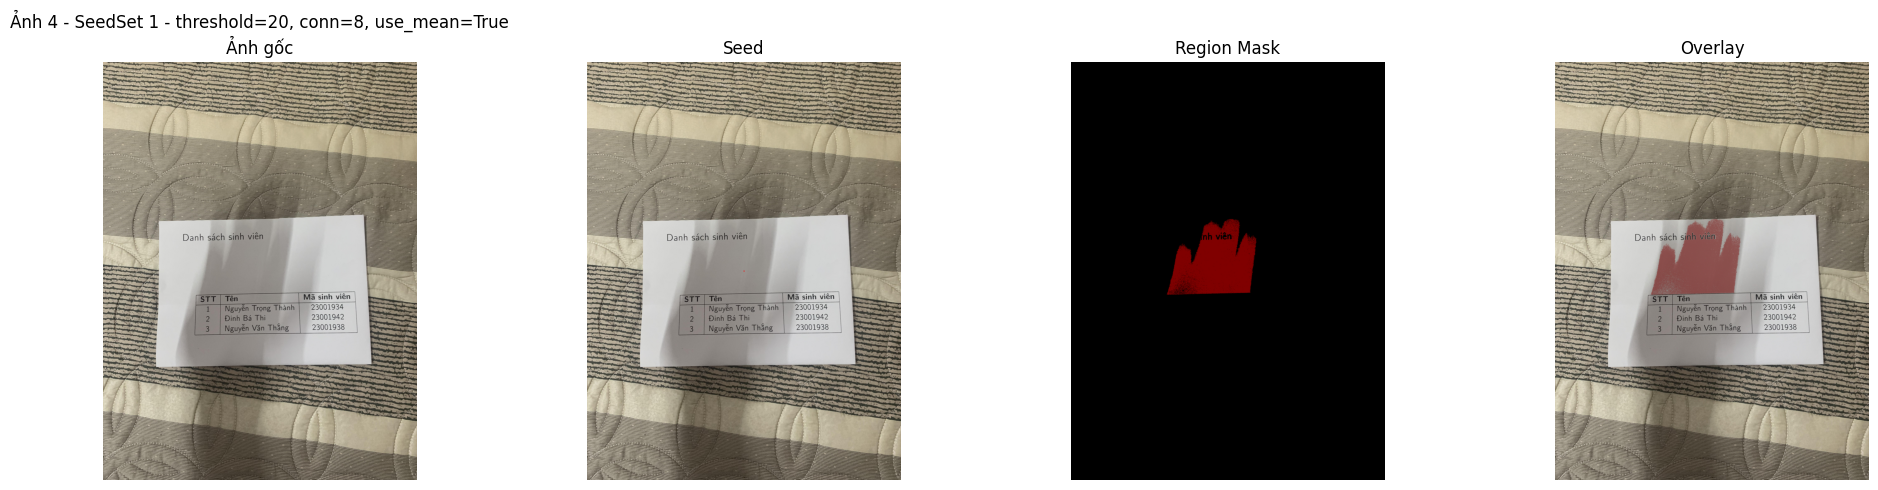
\includegraphics[width=\textwidth]{region2_20.png}
        \caption{Ảnh 4 với \texttt{threshold=20}}
    \end{subfigure}

    \vspace{0.2cm}

    \begin{subfigure}[b]{\textwidth}
        \centering
        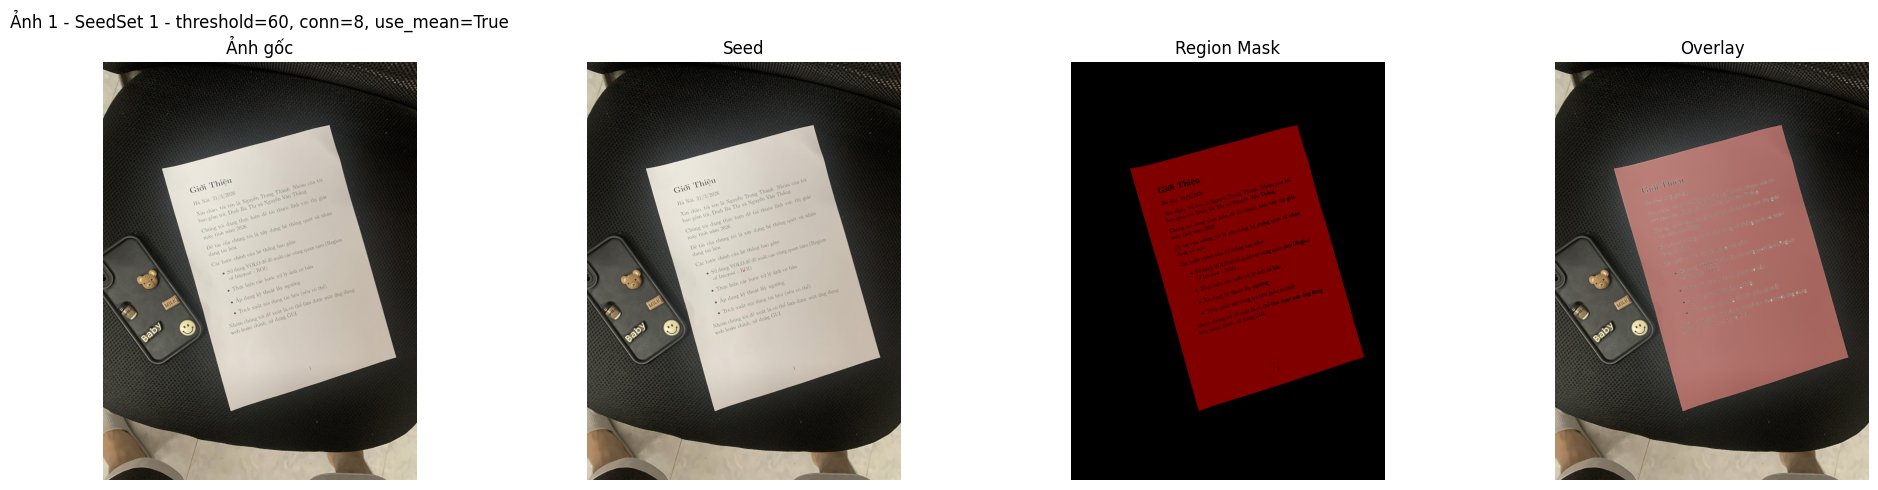
\includegraphics[width=\textwidth]{region1_60.png}
        \caption{Ảnh 1 với \texttt{threshold=60}}
    \end{subfigure}

    \vspace{0.2cm}

    \begin{subfigure}[b]{\textwidth}
        \centering
        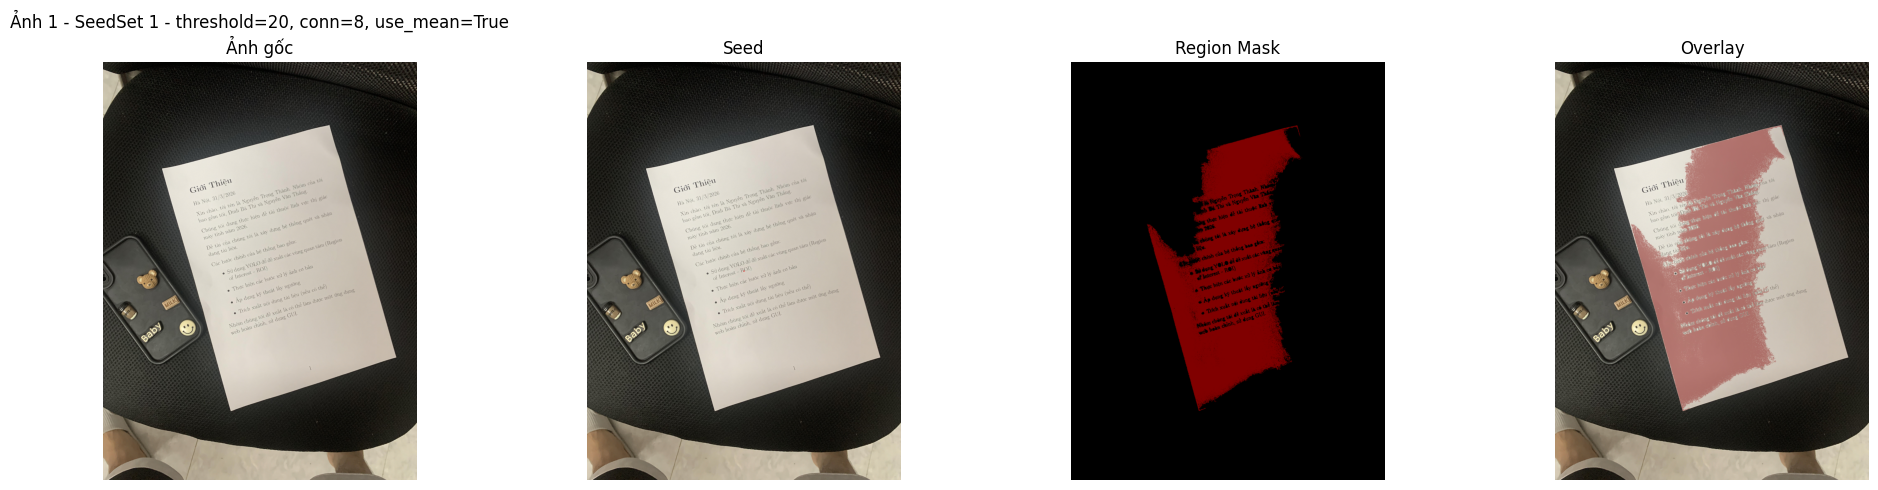
\includegraphics[width=\textwidth]{region1_20.png}
        \caption{Ảnh 1 với \texttt{threshold=20}}
    \end{subfigure}

    \caption{So sánh trực quan ảnh hưởng của ngưỡng \texttt{threshold} đến kết quả Region Growing trên ảnh RGB.}
    \label{fig:region-growing-threshold-comparison}
\end{figure}

Qua kết quả so sánh, ngưỡng \texttt{threshold} ảnh hưởng trực tiếp đến mức độ lan truyền vùng của Region Growing. Với \texttt{T=20}, thuật toán phát triển vùng thận trọng hơn nên vùng thu được nhỏ, dễ bị đứt gãy và bỏ sót nhiều phần của tài liệu. Ngược lại, với \texttt{T=60}, vùng được mở rộng hơn và có khả năng bao phủ tài liệu tốt hơn, nhưng trong một số trường hợp vẫn có thể bị ảnh hưởng bởi bóng đổ, chữ hoặc vùng có cường độ khác biệt lớn.

Trên ảnh màu được cân bằng sáng:


\begin{figure}[H]
    \centering
    
    \begin{subfigure}[b]{\textwidth}
        \centering
        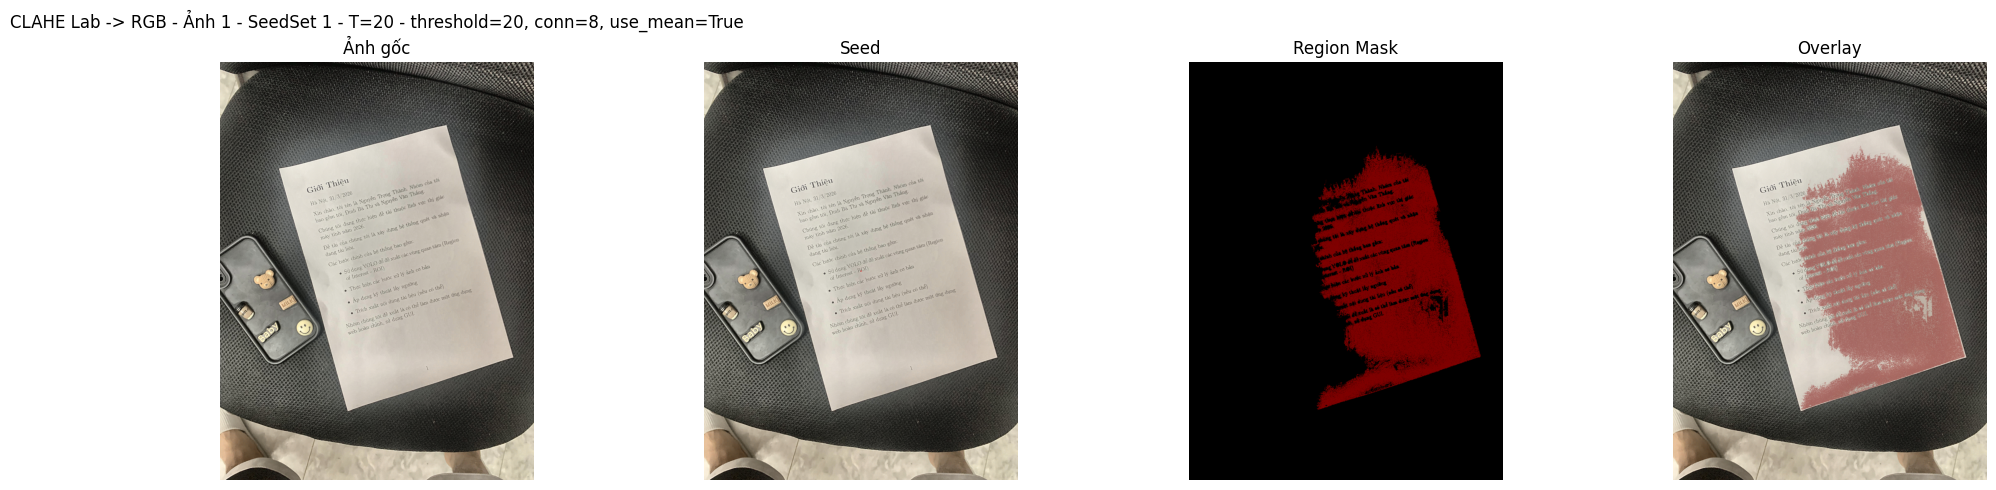
\includegraphics[width=\textwidth]{region_lab_ss1.png}
        \caption{Ảnh RGB với \texttt{threshold=20}}
    \end{subfigure}

    \vspace{0.2cm}

    \begin{subfigure}[b]{\textwidth}
        \centering
        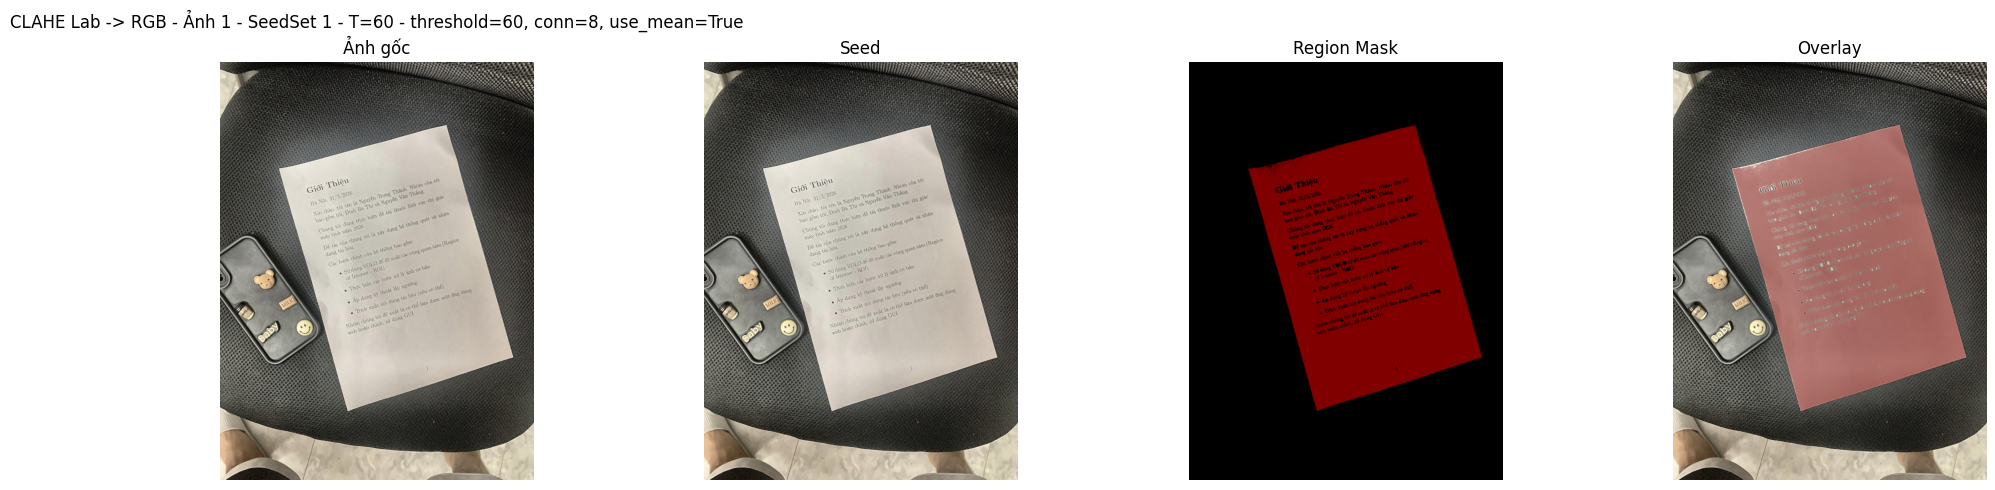
\includegraphics[width=\textwidth]{region_lab_ss2.png}
        \caption{Ảnh RGB với \texttt{threshold=60}}
    \end{subfigure}

    \caption{So sánh trực quan ảnh hưởng của ngưỡng \texttt{threshold} đến kết quả Region Growing trên ảnh RGB.}
    \label{fig:region-growing-rgb-threshold-comparison}
\end{figure}

Trên ảnh RGB, ngưỡng \texttt{threshold} quyết định trực tiếp phạm vi phát triển vùng. Với \texttt{T=20}, thuật toán chỉ giữ lại các pixel có màu sắc gần với seed nên vùng phân đoạn nhỏ và dễ bỏ sót các phần của tài liệu. Khi tăng lên \texttt{T=60}, vùng phát triển rộng hơn và bao phủ tài liệu tốt hơn. Tuy nhiên, nếu nền ảnh có màu gần với tài liệu, vùng cũng có thể lan sang các khu vực không mong muốn.

Trên ảnh xám:
\begin{figure}[H]
    \centering
    
    \begin{subfigure}[b]{\textwidth}
        \centering
        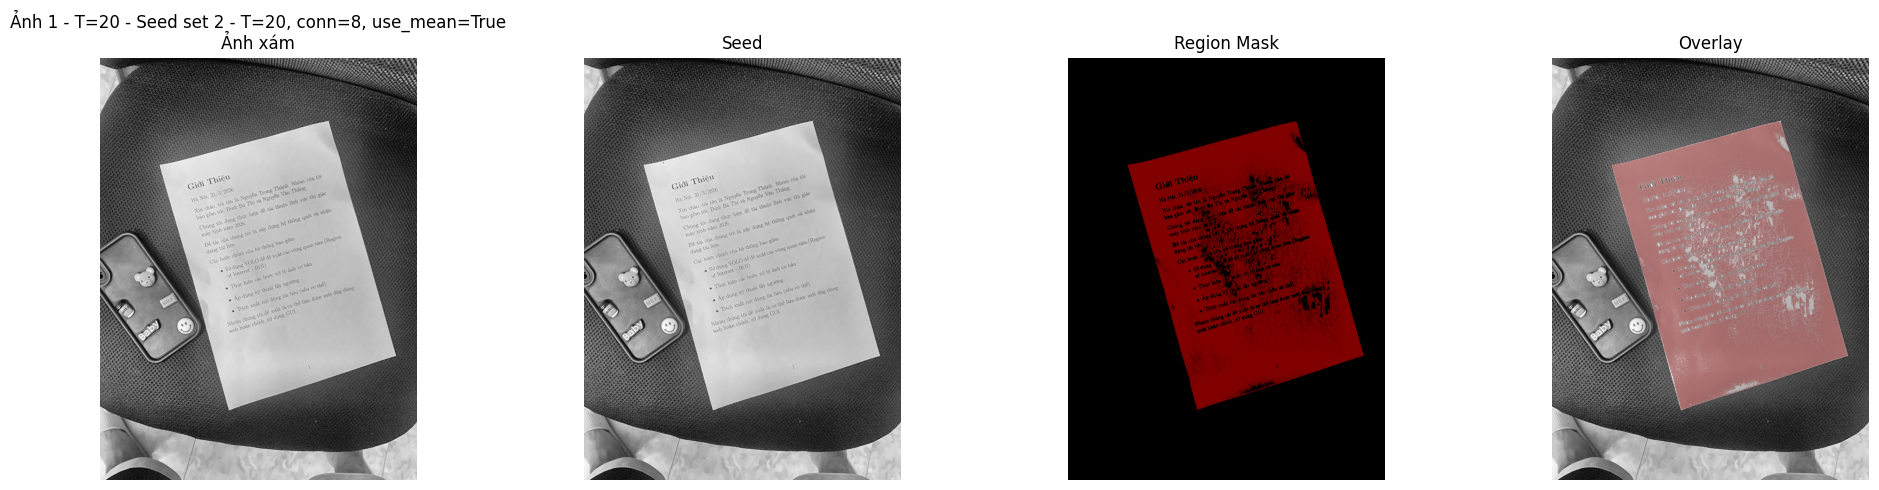
\includegraphics[width=\textwidth]{region_gray_ss1.png}
        \caption{Ảnh xám với \texttt{threshold=20}}
    \end{subfigure}

    \vspace{0.2cm}

    \begin{subfigure}[b]{\textwidth}
        \centering
        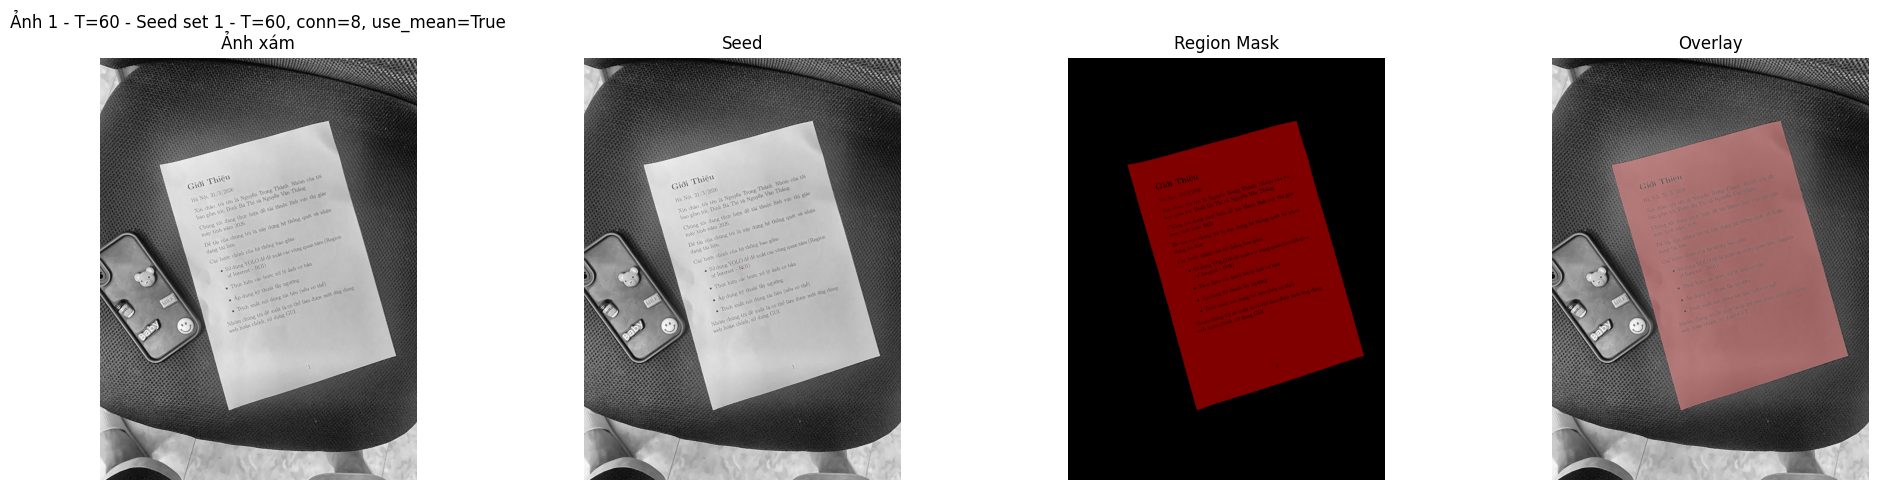
\includegraphics[width=\textwidth]{region_gray_ss2.png}
        \caption{Ảnh xám với \texttt{threshold=60}}
    \end{subfigure}

    \caption{So sánh trực quan ảnh hưởng của ngưỡng \texttt{threshold} đến kết quả Region Growing trên ảnh xám.}
    \label{fig:region-growing-gray-threshold-comparison}
\end{figure}

Qua kết quả so sánh, ngưỡng \texttt{threshold} ảnh hưởng rõ rệt đến khả năng lan truyền vùng của thuật toán Region Growing trên ảnh xám. Với \texttt{T=20}, thuật toán chỉ chấp nhận các pixel có mức xám gần giống với vùng mầm, nên vùng phân đoạn bị nhỏ, không đồng nhất và dễ bỏ sót nhiều phần của tài liệu, đặc biệt tại vùng chữ, bóng đổ hoặc vùng có thay đổi sáng tối. Ngược lại, với \texttt{T=60}, vùng được mở rộng tốt hơn và bao phủ gần như toàn bộ trang giấy, cho kết quả ổn định hơn. Tuy nhiên, nếu ngưỡng quá lớn, thuật toán vẫn có nguy cơ lan sang các vùng nền có cường độ gần giống với tài liệu.


\subsubsection{Ảnh hưởng bởi vị trí khởi tạo (Seed)}

\begin{figure}[H]
    \centering
    
    \begin{subfigure}[b]{\textwidth}
        \centering
        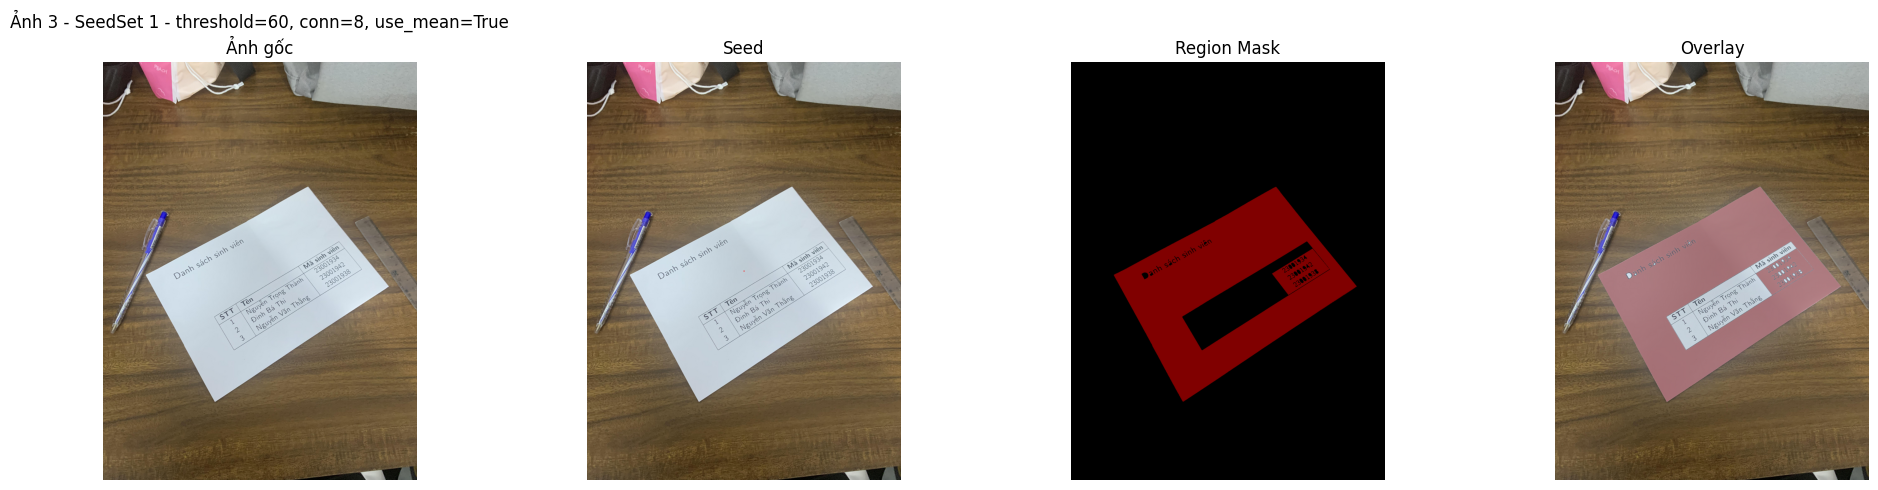
\includegraphics[width=\textwidth]{region5_s1.png}
        \caption{Ảnh 5 với \texttt{SeedSet 2}}
    \end{subfigure}

    \vspace{0.2cm}

    \begin{subfigure}[b]{\textwidth}
        \centering
        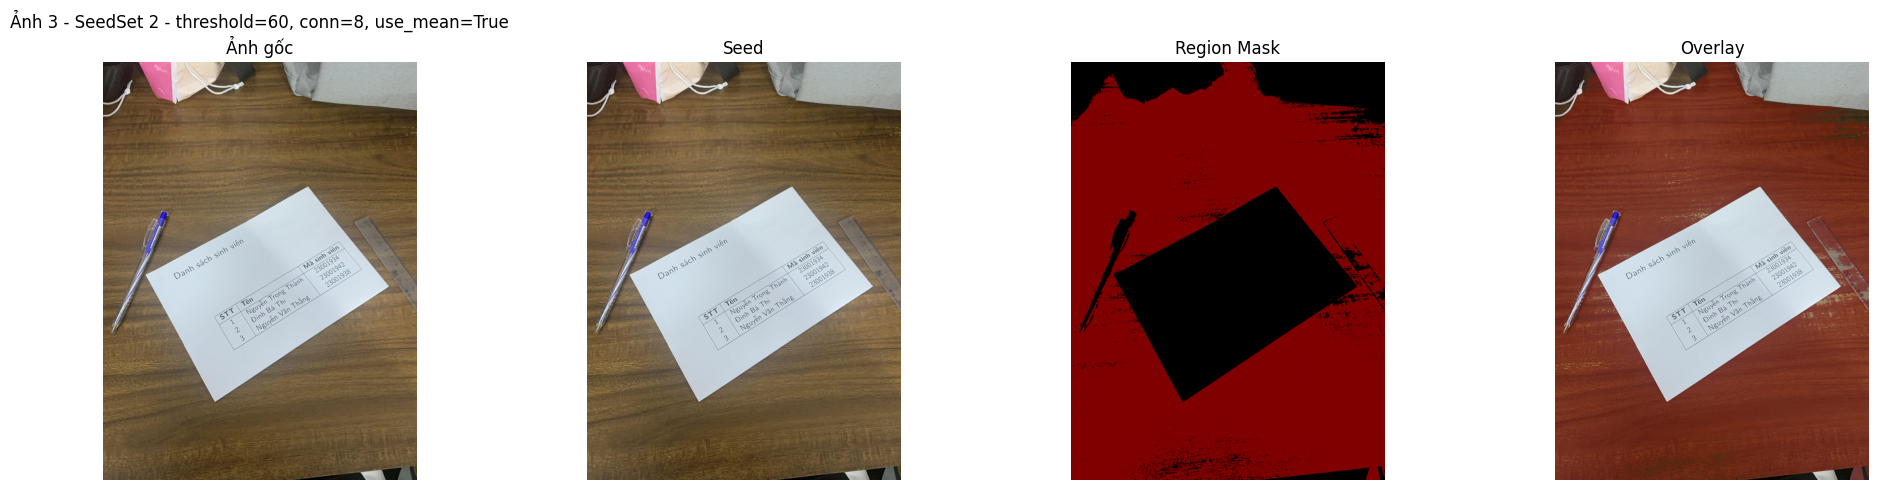
\includegraphics[width=\textwidth]{region5_s2.png}
        \caption{Ảnh 5 với \texttt{SeedSet 1}}
    \end{subfigure}

    \vspace{0.2cm}

    \begin{subfigure}[b]{\textwidth}
        \centering
        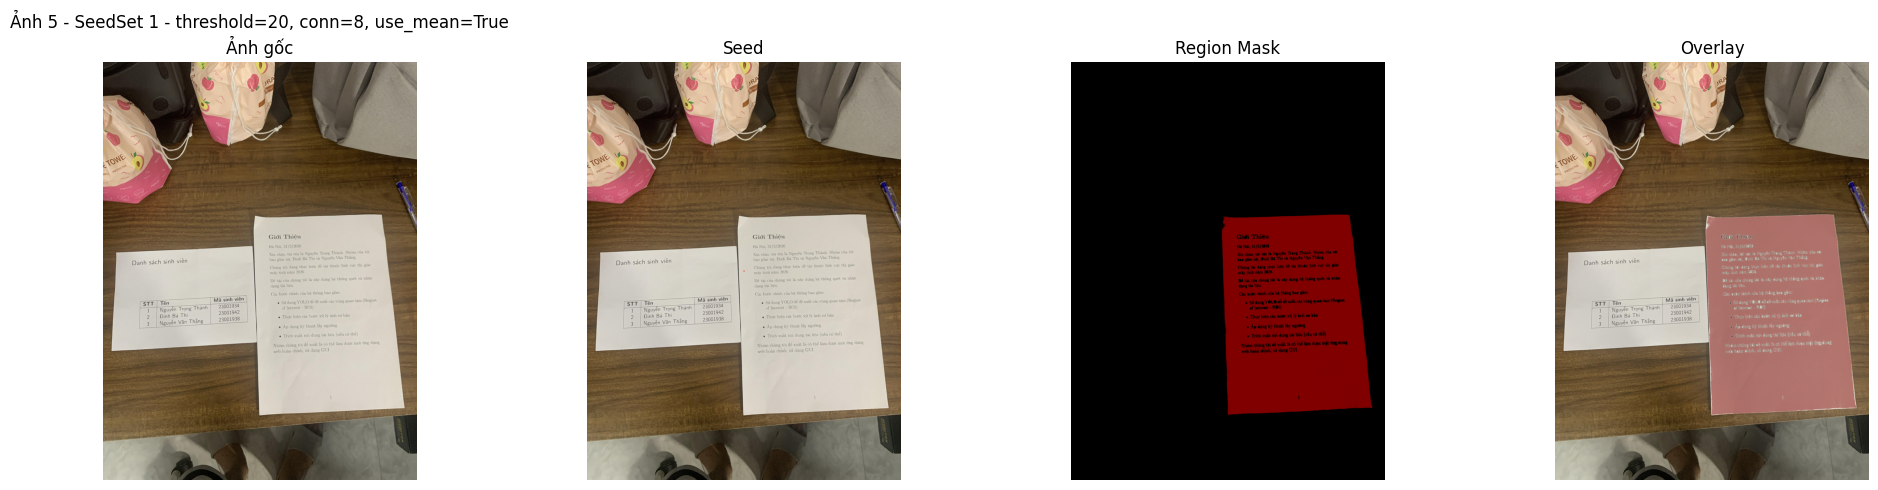
\includegraphics[width=\textwidth]{region6_s1.png}
        \caption{Ảnh 3 với \texttt{SeedSet 2}}
    \end{subfigure}

    \vspace{0.2cm}

    \begin{subfigure}[b]{\textwidth}
        \centering
        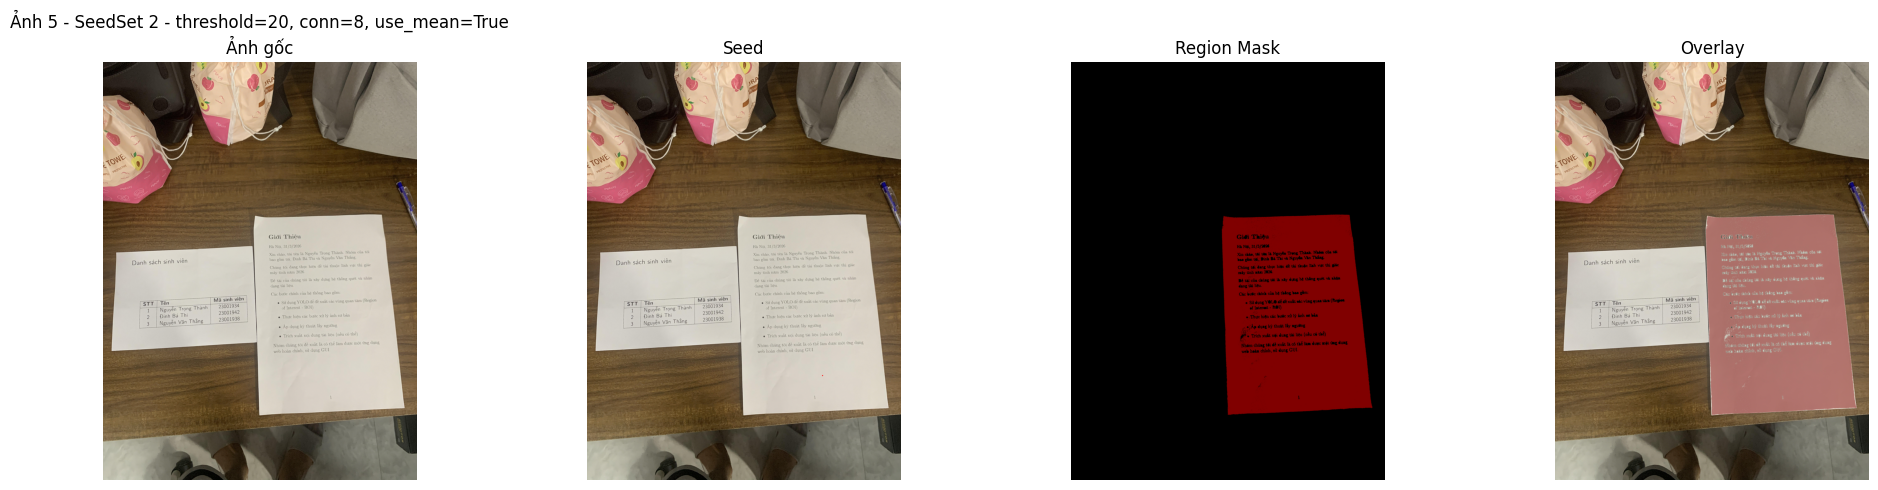
\includegraphics[width=\textwidth]{region6_s2.png}
        \caption{Ảnh 3 với \texttt{SeedSet 1}}
    \end{subfigure}

    \caption{So sánh trực quan ảnh hưởng của vị trí seed đến kết quả Region Growing.}
    \label{fig:region-growing-seed-comparison}
\end{figure}

Kết quả cho thấy cùng một ngưỡng nhưng thay đổi vị trí điểm mầm có thể làm vùng lan truyền khác đáng kể, từ đó ảnh hưởng trực tiếp đến khả năng bao phủ tài liệu.

Ảnh đầu 5, với 2 vị trí khởi tạo khác nhau là nền bàn, nền giấy, cho 2 kết quả khác nhau. Tương tự, với vị trí khởi tạo chỉ vào tài liệu bên phải, nên ảnh 3 không thể bắt được hoàn toàn 2 ảnh tài liệu.

\subsubsection{Nhận xét tổng thể}

Nhìn chung, Region Growing là thuật toán phân đoạn đơn giản, trực quan và dễ triển khai. Thuật toán hoạt động tốt khi điểm seed được đặt đúng trong vùng tài liệu và vùng cần tách có màu sắc hoặc cường độ tương đối đồng nhất. Với \texttt{connectivity=8} và cơ chế cập nhật trung bình vùng động, thuật toán có thể lan truyền linh hoạt hơn, giúp bao phủ tốt các vùng giấy có sự thay đổi sáng nhẹ.

Tuy nhiên, kết quả của Region Growing phụ thuộc mạnh vào vị trí seed và giá trị ngưỡng \texttt{threshold}. Nếu ngưỡng quá nhỏ, vùng phân đoạn dễ bị đứt gãy và bỏ sót; nếu ngưỡng quá lớn, thuật toán có thể lan sang nền hoặc các vùng không mong muốn. Ngoài ra, với ảnh có bóng đổ mạnh, nền phức tạp hoặc nhiều chi tiết chữ/bảng biểu, thuật toán dễ cho kết quả không ổn định. Do phải duyệt từng pixel và kiểm tra láng giềng liên tục, Region Growing cũng có chi phí tính toán lớn khi xử lý ảnh độ phân giải cao.

\section{Phân tích và thảo luận}

Qua các thực nghiệm, có thể thấy bài toán scan tài liệu phụ thuộc mạnh vào chất lượng ảnh đầu vào, đặc biệt là ánh sáng, bóng đổ, độ tương phản giữa giấy và nền, cũng như mức độ phức tạp của nền. Không có một phương pháp duy nhất hoạt động tốt trong mọi trường hợp, mà mỗi thuật toán đều có ưu điểm và hạn chế riêng.

Đối với tiền xử lý, CLAHE giúp cải thiện độ tương phản cục bộ, làm rõ vùng giấy và nét chữ trong các ảnh thiếu sáng hoặc có bóng đổ. Tuy nhiên, nếu nền ảnh có nhiều họa tiết như vân gỗ, vải hoặc ghế lưới, CLAHE cũng có thể khuếch đại các chi tiết nền, làm tăng nhiễu cho bước phát hiện biên và phân đoạn.

Trong phát hiện biên, ảnh xám và kênh sáng của hệ LAB cho kết quả ổn định hơn so với việc xử lý trực tiếp trên nhiều kênh màu. Việc gộp biên từ RGB hoặc HSV có thể giữ lại nhiều chi tiết hơn, nhưng đồng thời cũng làm cộng dồn nhiễu từ nền. Do đó, với mục tiêu chính là tìm khung viền tài liệu, xử lý trên ảnh Gray hoặc LAB kết hợp ngưỡng phù hợp là lựa chọn an toàn hơn.

Ở bước tìm contour, chất lượng ảnh biên đóng vai trò quyết định. Nếu biên quá nhiễu, thuật toán sẽ sinh nhiều contour rác; nếu biên bị đứt gãy, contour tài liệu không thể khép kín. Các phép biến đổi hình thái học, đặc biệt là Close rồi Open với kích thước kernel vừa phải, giúp nối các đoạn biên bị hở và loại bỏ nhiễu nhỏ, từ đó cải thiện khả năng xác định vùng tài liệu.

Đối với các phương pháp phân đoạn, K-Means với $K=2$ cho kết quả phù hợp hơn vì bài toán chủ yếu cần tách tài liệu khỏi nền. Khi tăng lên $K=3$, thuật toán dễ phân tách thêm bóng đổ, chữ hoặc chi tiết nền, dẫn đến hiện tượng phân mảnh. Watershed có khả năng tách vùng tốt trong một số trường hợp, nhưng lại quá nhạy với chữ viết, bóng đổ và texture nền, gây over-segmentation và làm mất cấu trúc tứ giác của tài liệu. Region Growing cho kết quả trực quan và có thể tạo vùng liền mạch, nhưng phụ thuộc mạnh vào vị trí seed và ngưỡng threshold; nếu chọn không phù hợp, vùng có thể bị thiếu hoặc lan sang nền.

Nhìn chung, các phương pháp xử lý ảnh truyền thống có ưu điểm là dễ triển khai, dễ quan sát và không cần dữ liệu huấn luyện. Tuy nhiên, hệ thống vẫn phụ thuộc nhiều vào tham số như ngưỡng, kernel, seed và điều kiện chụp ảnh. Đây là hạn chế lớn khi triển khai trên dữ liệu thực tế đa dạng. Vì vậy, hướng cải thiện trong tương lai là kết hợp thêm các phương pháp học sâu để tăng khả năng tổng quát hóa trong các trường hợp nền phức tạp, bóng đổ mạnh hoặc tài liệu bị che khuất.


\chapter{Kết luận và hướng phát triển} 
\section{Kết luận}

Dự án đã xây dựng thành công một hệ thống tự động nhận diện và scan tài liệu vận hành hoàn toàn dựa trên sự tinh tế của các thuật toán Xử lý ảnh số truyền thống. Bằng cách thao túng sự tách biệt ánh sáng trong hệ tọa độ màu HSV và LAB, hệ thống giải quyết trọn vẹn rắc rối do ánh sáng môi trường. Sự phối hợp của các bộ lọc CLAHE, màng lọc hình thái học Opening/Closing, định vị biên đa kênh và các biến đổi uốn góc Homography đã đáp ứng chính xác nhu cầu số hóa tài liệu.

Bên cạnh đó, dự án đã mạnh dạn ứng dụng và phân tích mổ xẻ những thiết kế phức tạp trong phân đoạn ảnh bậc cao. Trong khi Marker-Controlled Watershed khống chế hoàn toàn bài toán Over-segmentation đem lại biên viền tách biệt, Region Growing mở ra khả năng thích ứng linh hoạt với đổ bóng nhưng đồng thời bộc lộ yếu điểm về mặt quản lý tài nguyên tính toán không gian.
 
\section{Hướng phát triển}

Mặc dù các phương pháp kỹ thuật tính toán truyền thống đóng vai trò xương sống cho việc phân tích, sự phụ thuộc vào các ngưỡng (thresholds) cấu hình tĩnh vẫn làm giảm khả năng khái quát (generalization) của hệ thống trong những điều kiện che khuất nghiêm trọng. 

Hướng phát triển mũi nhọn trong thời gian tới là tích hợp các mô hình Học sâu (Deep Learning) như U-Net \cite{unet2015}, Mask R-CNN \cite{maskrcnn2017} hay các mô hình trích xuất đặc trưng không gian đa lớp. Những mô hình mạng Nơ-ron tích chập này có khả năng tự động học hỏi những đặc trưng ngữ nghĩa của văn bản mà không bị ràng buộc bởi sự đồng nhất màu sắc, hứa hẹn sẽ mang đến khả năng bao quát tài liệu dẫu cho giấy có bị che bởi các vật dụng cá nhân, gập nếp, rách viền hay điều kiện ánh sáng cực kỳ bất lợi. 

Thêm vào đó, để khắc phục hiện tượng OOM của thuật toán Region Growing, việc tối ưu hóa nhân mã Python bằng cách tích hợp trực tiếp với các module biên dịch C/C++ thông qua Cython \cite{cython_docs} hoặc PyBind là một lối thoát khả thi cho việc triển khai ở thời gian thực.

\clearpage % Đẩy phần Tài liệu tham khảo sang một trang mới
\addcontentsline{toc}{chapter}{Tài liệu tham khảo}
% \chapter*{Tài liệu tham khảo}
\begin{thebibliography}{99}

% --- Tài liệu thư viện (OpenCV, NumPy) ---
\bibitem{opencv_docs}
OpenCV Developers, ``OpenCV-Python Tutorials,'' OpenCV Documentation. [Online]. Available: \url{https://docs.opencv.org/}. [Accessed: May 2026].

\bibitem{clahe1994}
K. Zuiderveld, ``Contrast Limited Adaptive Histogram Equalization,'' in \textit{Graphics Gems IV}, San Diego, CA, USA: Academic Press Professional, Inc., 1994, pp. 474-485.

% --- Sách giáo khoa kinh điển (Dành cho Region Growing, Morphology, Homography, Color Spaces) ---
\bibitem{gonzalez2018}
R. C. Gonzalez and R. E. Woods, \textit{Digital Image Processing}, 4th ed. Pearson, 2018.

% --- Bài báo gốc của các thuật toán tiền xử lý & phân đoạn truyền thống ---
\bibitem{canny1986}
J. Canny, ``A Computational Approach to Edge Detection,'' \textit{IEEE Transactions on Pattern Analysis and Machine Intelligence}, vol. 8, no. 6, pp. 679-698, Nov. 1986.

\bibitem{otsu1979}
N. Otsu, ``A Threshold Selection Method from Gray-Level Histograms,'' \textit{IEEE Transactions on Systems, Man, and Cybernetics}, vol. 9, no. 1, pp. 62-66, Jan. 1979.



% --- Bài báo gốc cho hướng phát triển Deep Learning (Chương 4) ---
\bibitem{unet2015}
O. Ronneberger, P. Fischer, and T. Brox, ``U-Net: Convolutional Networks for Biomedical Image Segmentation,'' in \textit{Medical Image Computing and Computer-Assisted Intervention (MICCAI)}, 2015, pp. 234-241.

\bibitem{maskrcnn2017}
K. He, G. Gkioxari, P. Dollar, and R. Girshick, ``Mask R-CNN,'' in \textit{Proceedings of the IEEE International Conference on Computer Vision (ICCV)}, 2017, pp. 2961-2969.

% --- Công cụ tối ưu hóa ---
\bibitem{cython_docs}
Cython Developers, ``Cython: C-Extensions for Python,'' [Online]. Available: \url{https://cython.org/}. [Accessed: May 2026].

% --- Tài liệu nội bộ trường ---
% \bibitem{baigiang_tgmt}
% C. V. Chung, ``Bài giảng môn Thị giác máy tính,'' Khoa Toán - Cơ - Tin học, Trường Đại học Khoa học Tự nhiên, Hà Nội, 2026.

\end{thebibliography}
% --- KẾT THÚC TÀI LIỆU ---
\end{document}
